\documentclass[a4paper,12pt]{scrreprt}

\usepackage[margin=1in]{geometry}
\usepackage{amsmath}
\usepackage{amsfonts}
\usepackage{amssymb}
\usepackage{fancyhdr}
\usepackage{amstext}
\usepackage{array}
\usepackage{amsthm}
\usepackage{tikz}
\usepackage{bm}
\usepackage{mathrsfs}
\usepackage{mathrsfs}
\usepackage{eucal}
\usepackage{braket}
\usepackage{pgfplots}
\usepackage{soul}
\usepackage{hyperref}
\usepackage{todonotes}
\usepackage{enumitem}
\usepackage{braids}
\usepackage{epigraph}
\usepackage[compat=1.1.0]{tikz-feynman}
\usepackage{xcolor}
\usepackage{appendix}
\usepackage{libertine}
\usepackage[libertine]{newtxmath}
\usepackage{microtype}
\usepackage{anyfontsize}
\usepackage{interval}

% chktex-file 18
% chktex-file 6
% chktex-file 34

% Set up hyperref colors
\hypersetup{
    colorlinks,
    linkcolor={blue!50!black},
    citecolor={blue!50!black},
    urlcolor={blue!80!black}
}

% Good practice to set the version so updates don't break old documents
\pgfplotsset{compat=1.14}

% Open intervals should use parentheses
\intervalconfig{soft open fences}

% Load tikz-cd
\usetikzlibrary{cd}
\usetikzlibrary{external}

% Declares the font calligra
\usepackage{calligra}
\DeclareMathAlphabet{\mathcalligra}{T1}{calligra}{m}{n}
\DeclareFontShape{T1}{calligra}{m}{n}{<->s*[2.2]callig15}{}

% Makes '\sr' a script r
\newcommand{\sr}{r}

% Makes indentation more note-ish
\setlength{\parindent}{0em}
\setlength{\parskip}{.5em}
\setlength{\headheight}{14.0pt}

% My commands
\newcommand{\pder}[2]{\frac{\partial #1}{\partial #2}}
\newcommand{\tder}[2]{\frac{d #1}{d #2}}
\newcommand{\R}{\mathbb{R}}
\newcommand{\C}{\mathbb{C}}
\newcommand{\Z}{\mathbb{Z}}
\newcommand{\Q}{\mathbb{Q}}
\newcommand{\N}{\mathbb{N}}
\newcommand{\dd}{\mathrm{d}}
\newcommand{\defn}[1]{\ul{#1}}
\newcommand{\cliff}{\mathrm{C}\ell}
\newcommand{\Ad}{\mathrm{Ad}}
\newcommand{\tAd}{\widetilde{\mathrm{Ad}}}
\newcommand{\Pin}{\mathrm{Pin}}
\newcommand{\Spin}{\mathrm{Spin}}
\newcommand{\Or}{\mathrm{O}}
\newcommand{\SO}{\mathrm{SO}}
\newcommand{\SL}{\mathrm{SL}}
\newcommand{\SU}{\mathrm{SU}}
\newcommand{\PP}{\mathrm{P}}
\newcommand{\tP}{\tilde{\mathrm{P}}}
\newcommand{\SP}{\mathrm{SP}}
\newcommand{\GL}{\mathrm{GL}}
\newcommand{\Obj}{\mathrm{Obj}}
\newcommand{\Hom}{\mathrm{Hom}}
\newcommand{\Nat}{\mathrm{Nat}}
\newcommand{\Line}{\mathrm{Line}}
\newcommand{\ev}{\mathrm{eval}}
\newcommand{\coker}{\mathrm{coker}}
\newcommand{\im}{\mathrm{im}}
\newcommand{\Mor}{\mathrm{Mor}}
\newcommand{\dom}{\mathrm{dom}}
\newcommand{\cod}{\mathrm{cod}}
\newcommand{\norm}[1]{\left\lVert#1\right\rVert}
\newcommand{\End}{\mathrm{End}}
\newcommand{\Aut}{\mathrm{Aut}}
\newcommand{\Spec}{\mathrm{Spec}}
\newcommand{\spec}{\mathrm{Spec}}
\newcommand{\id}{\mathrm{id}}
\newcommand{\abs}[1]{\left|#1\right|}

% Hyphen for names of categories
\def\mhyp{{\hbox{-}}}

% Second level of list uses empty bullets
\renewcommand{\labelitemii}{$\circ$}

% Declare theorem styles
\theoremstyle{definition}
\newtheorem{definition}{Definition}
\newtheorem{example}[definition]{Example}
\newtheorem{recurring_example}[definition]{Recurring Example}
\newtheorem{counterexample}[definition]{Counterexample}
\newtheorem{fact}[definition]{Fact}

\theoremstyle{plain}
\newtheorem{theorem}[definition]{Theorem}
\newtheorem{lemma}[definition]{Lemma}
\newtheorem{corollary}[definition]{Corollary}
\newtheorem{proposition}[definition]{Proposition}

\theoremstyle{remark}
\newtheorem{claim}[definition]{Claim}
\newtheorem{recipe}[definition]{Recipe}
\newtheorem{note}[definition]{Note}
\newtheorem{notation}[definition]{Notation}
\newtheorem{joke}[definition]{Joke}

\title{Category theory notes}
\author{Angus Rush}

\begin{document}
\maketitle
\tableofcontents
%\tikzexternalize[prefix=figures/]

\chapter{Basic category theory}\label{ch:categories}

\section{Categories}\label{sec:categoriesbasicdefinitions}
There are lots of different sorts of mathematical structures, each of which is good for different things. Groups are good for talking about symmetries, for instance, and rings are good for talking about function fields.

Categories are just another type of mathematical structure, but they have a different, more abstract feel to them than groups or rings. One reason for this is that they are inherently meta-mathematical: they are good for talking about other mathematical objects, and the relationships between them.

For this reason, category theory has developed a reputation for being abstract and difficult to learn, which is mostly undeserved. Categories are nothing special; they are mathematical objects, just like groups or vector spaces. They are simply good for different things.

\subsection{Basic definitions}
Unfortunately, there are many different conventions regarding how to typeset category theory. I will do my best to stick to the conventions used at the nLab (\cite{nlab}).

\begin{definition}[category]\label{def:category}
  A \defn{category} $\mathsf{C}$ consists of the following pieces of data.
  \begin{itemize}
    \item A collection\footnote{There is a reason we say that there is a \emph{collection}, rather than a \emph{set}, of objects (and morphisms): it may be that there may be `too many' objects (or morphisms) to be contained in a set. For example, there is no set of all sets, but we will see that there is a category of sets. We will for the most part sidestep foundational questions of size, but in some cases it will be unavoidable. In particular, categories whose objects and/or morphisms \emph{are\/} small enough to be contained in a set will play an especially important role.} $\Obj(\mathsf{C})$ of \emph{objects}.
    \item For every two objects $A$, $B \in \Obj(\mathsf{C})$, a collection $\Hom(A,B)$ of \emph{morphisms\/} with the following properties.
      \begin{enumerate}
        \item\label{item:compositionofmorphisms} For any $f \in \Hom(A,B)$ and $g \in \Hom(B,C)$, there is an associated morphism
          \begin{equation*}
            g \circ f \in \Hom(A,C),
          \end{equation*} called the \emph{composition\/} of $f$ and $g$.

        \item This composition is associative: $(f \circ g) \circ h = f \circ (g \circ h)$.

        \item\label{item:existenceofidentitymorphism} For every $A \in \Obj(\mathsf{C})$, there is at least one morphism $1_{A}$, called the \emph{identity morphism\/} which functions as both a left and right identity with respect to the composition of morphisms, i.e.\
          \begin{equation*}
            f \circ 1_{A} = f\qquad\text{amd}\qquad 1_{A} \circ g = g.
          \end{equation*}
      \end{enumerate}
  \end{itemize}

  If ever it is potentially unclear which category we are talking about, we will add a subscript to $\Hom$, writing for example $\Hom_{\mathsf{C}}(A,B)$ instead of $\Hom(A,B)$.
\end{definition}

\begin{notation}
  Following Aluffi (\cite{aluffi-algebra-chapter-0}), we will use a sans serif font to denote categories. For example $\mathsf{C}$, $\mathsf{Set}$.
\end{notation}

One thinks of morphisms as `generalized functions.' It is therefore often useful to use functional notation $f\colon A \to B$ to describe morphisms. For example, the following two notations are equivalent:
\begin{equation*}
  f \in \Hom(A, B) \iff f\colon A \to B.
\end{equation*}

Here is something to be aware of: the identity morphism $1_{A}\colon A \to A$ is often simply denoted by $A$. This is actually a good notation, and we will use it freely in later chapters. However, we will avoid it in earlier chapters since it is potentially confusing whether we are talking about $A$ the object or $A$ the morphism.
\subsubsection*{Some examples of categories}\label{sss:examples_of_categories}

The idea of a category is very abstract. Examples of categories abound; we give only a few here.

\begin{example}[The category of sets]
  The prototypical category is $\mathsf{Set}$, the category whose objects are sets and whose morphisms are set functions.

  In order to check that $\mathsf{Set}$ is indeed a category, we need to check that the axioms are satisfied. In fact, everything is more or less clear by definition.

  A category first needs a collection of objects. Although there is no set of sets, there certainly is a collection of all sets. Therefore,
  \begin{equation*}
    \Obj(\mathsf{Set}) = [\text{all sets}].
  \end{equation*}

  The next thing a category needs is, for each pair of objects $A$, $B$, a collection of morphisms $\Hom_{\mathsf{Set}}(A, B)$. The morphisms between the objects in $\mathsf{Set}$, i.e.\ sets, will consist of all set-functions between. That is,
  \begin{equation*}
    \Hom_{\mathsf{Set}}(A, B) = \{f\colon A \to B\ |\ f\ \text{is a set function.}\}
  \end{equation*}

  Functions can indeed be composed, and this composititon is associative. Furthermore, every set has an identity which maps every element to itself.
\end{example}

\begin{example}[category with one object]\label{eg:categorywithoneobject}
  The category $\mathsf{1}$, where $\Obj(\mathsf{1})$ is the singleton $\{*\}$, and the only morphism is the identity morphism $\mathrm{id}_{*}\colon * \to *$.
\end{example}

Categories capture the essence of `things and composable maps between them.' There are many mathematical structures which naturally come with a notion of map between them, usually called homomorphisms. These are almost always composable, which means it is often natural to imagine them as living in their own categories.
\begin{example}\label{eg:examplesofcategories}
  If you know what the following mathematical objects are, it is nearly effortless to check that they are categories.\footnote{Look at the definition. It \emph{really is} trivial.}
  \begin{itemize}
    \item $\mathsf{Grp}$, whose objects are groups and whose morphisms are group homomorphisms.

    \item\label{item:categoryab} $\mathsf{Ab}$, whose objects are abelian groups and whose morphisms are group homomorphisms.

    \item $\mathsf{Ring}$, whose objects are rings and whose morphisms are ring homomorphisms.

    \item $R\mhyp\mathsf{Mod}$, whose objects are modules over a ring $R$ and whose morphisms are module homomorphisms.

    \item $\mathsf{Vect}_{k}$, whose objects are vector spaces over a field $k$ and whose morphisms are linear maps.
    \item $\mathsf{FinVect}_{k}$, whose objects are finite-dimensional vector spaces over a field $k$ and whose morphisms are linear maps.
    \item $k\mhyp\mathsf{Alg}$, whose objects are algebras over a field $k$ and whose morphisms are algebra homomorphisms.
  \end{itemize}
\end{example}

\begin{example}\label{eg:moreexamplesofcategories}
  In addition to algebraic structures, categories help to talk about geometrical structures. The following are also categories.
  \begin{itemize}
    \item $\mathsf{Top}$, whose objects are topological spaces and whose morphisms are continuous maps.
    \item $\mathsf{Met}$, whose objects are metric spaces and whose morphisms are metric maps.
    \item $\mathsf{Man}^{p}$, whose objects are manifolds of class $C^{p}$ and whose morphisms are $p$-times differentiable functions.

    \item $\mathsf{SmoothMfd}$, whose objects are $C^{\infty}$ manifolds and whose morphisms are smooth functions.
  \end{itemize}
\end{example}

\begin{example}\label{eg:groupsaregroupoidswithoneobject}
  Here is a slightly whimsical example of a category, which is different in nature to the other categories we've looked at before. This category is important when studying group representations.

  Let $G$ be a group. We are going to create a category $\mathsf{G}$ which behaves like this group.
  \begin{itemize}
    \item Our category $\mathsf{G}$ has only one object, called $*$.

    \item The set $\Hom_{\mathsf{G}}(*, *)$ is equal to the underlying set of the group $G$, and for $f$, $g \in \Hom_{\mathsf{G}}(*, *)$, the compositions $f \circ g = f\cdot g$, where $\cdot$ is the group operation in $G$. The identity $e \in G$ is the identity morphism $1_{*}$ on $*$.
  \end{itemize}
  \begin{equation*}
    \begin{tikzcd}
      *
      \arrow[loop right, "e = 1_{*}"]
      \arrow[loop above, "g"]
      \arrow[loop left, "f"]
      \arrow[loop below, "g \circ f"]
    \end{tikzcd}
  \end{equation*}
\end{example}
\subsubsection{Commutative diagrams}\label{sss:commutative_diagrams}

It is often helpful to visualize objects and morphisms in categories using as so-called \emph{multidigraphs,}\footnote{A multidigraph is a directed graph which is allowed to have more than one edge between any given pair of vertices.} with the objects as vertices and the morphisms as edges. This makes it possible to visualize categories by drawing graph-like diagrams. Scroll to almost any page in this document, and you will likely see a diagram or two which resemble this one (copied directly from \hyperref[def:pullback]{Definition~\ref*{def:pullback}}).
\begin{equation*}
  \begin{tikzcd}
    V \arrow[rrd, bend left, "t"] \arrow[rd, dashed, "\exists!h"] \arrow[rdd, bend right, swap, "s"] &   &  \\
    & U \arrow[r, "q"] \arrow[d, swap, "p"] & B \arrow[d, "g"] \\
    & A \arrow[r, swap, "f"] & C
  \end{tikzcd}
\end{equation*}
Category theorists frequently employ these diagrams, called \emph{commutative diagrams,}\footnote{We will define later when a diagram does or does not commute. Annoyingly, even diagrams which don't commute are called commutative diagrams.} to make the ideas beind a proof more clear. Many results in category theory are most easily proved by drawing such a diagram, and then pointing at edges and vertices while repeating the phrase `and then this goes here,' while furrowing one's brow. This form of proof is called a `diagram chase,' and category theorists are very fond of them.


\subsection{Building new categories from existing ones}
One of the first things one learns about when talking about a mathematical structure is how to use existing ones to create new ones. For example, one can take the product of two groups to create a third, or take the quotient a vector space by a subspace. Categories are no exception. In this section, we will learn how to create new categories out of old categories.

The first way we'll see of doing this may seem a bit trivial.

\begin{definition}[opposite category]\label{def:oppositecategory}
  Let $\mathsf{C}$ be a category. Its \defn{opposite category} $\mathsf{C}^{\mathrm{op}}$ is the category whose objects are the same as the objects $\Obj(\mathsf{C})$ and whose morphisms $f \in \Hom_{\mathsf{C}^{\mathrm{op}}}(A, B)$ are defined to be the morphisms $\Hom_{\mathsf{C}}(B, A)$.

  That is to say, the opposite category is the category one gets by formally reversing all the arrows in a category. If $f \in \Hom_{\mathsf{C}}(A, B)$, i.e. $f \colon A \to B$, then in $\mathsf{C}^{\mathrm{op}}$, $f\colon B \to A$.
\end{definition}

This may seem like an uninterersting, definition, but having it around will make life a lot easier when it comes to defining functors (\hyperref[sec:functors]{Section~\ref*{sec:functors}}).

One can take the Cartesian product of two sets by creating ordered pairs. One can also take the product of two categories, which works in the way one would likely expect.

\begin{definition}[product category]\label{def:productcategory}
  Let $\mathsf{C}$ and $\mathsf{D}$ be categories. The \defn{product category} $\mathsf{C} \times \mathsf{D}$ is the following category.
  \begin{itemize}
    \item The objects $\Obj(\mathsf{C} \times \mathsf{D})$ consist of all ordered pairs $(C, D)$, where $C \in \Obj(\mathsf{C})$ and $D \in \Obj(\mathsf{D})$.

    \item For any two objects $(C, D)$, and $(C', D') \in \Obj(\mathsf{C} \times \mathsf{D})$,
      the morphisms $\Hom_{C \times D}((C, D), (C', D'))$ are ordered pairs $(f,g)$, where $f \in \Hom_{\mathsf{C}}(C, C')$ and $g \in \Hom_{\mathsf{D}}(D, D')$.

    \item Composition is taken componentwise, so that
      \begin{equation*}
        (f_{1}, g_{1}) \circ (f_{2},g_{2}) = (f_{1} \circ g_{1}, f_{2} \circ g_{2}).
      \end{equation*}

    \item The identity morphisms are given in the obvious way:
      \begin{equation*}
        1_{(C,D)} = (1_{C}, 1_{D}).
      \end{equation*}
  \end{itemize}
\end{definition}

Many mathematical objects have a notion of `sub-object.' For example, groups can have subgroups, and vector spaces can have vector subspaces. Categories also have this notion. As with groups and vector spaces, the definition of a `subcategory' is more or less obvious, but it is helpful to know exactly what one has to check to show that a subcollection of objects and morphisms from a category forms a subcategory.

\begin{definition}[subcategory]\label{def:subcategory}
  Let $\mathsf{C}$ be a category. A category $\mathsf{S}$ is a \defn{subcategory} of $\mathsf{C}$ if the following conditions hold.
  \begin{itemize}
    \item The objects $\Obj(\mathsf{S})$ of $\mathsf{S}$ are a subcollection of the objects of $\mathsf{C}$.

    \item For $S$, $T \in \Obj(\mathsf{S})$, the morphisms $\Hom_{\mathsf{S}}(S, T)$ are a subcollection of the morphisms $\Hom_{\mathsf{C}}(S, T)$ which satisfy the following.
      \begin{itemize}
        \item For every $S \in \Obj(S)$, the identity $1_{S} \in \Hom_{\mathsf{S}}(S, S)$.

        \item For all $f \in \Hom_{\mathsf{S}}(S, T)$ and $g \in \Hom_{\mathsf{S}}(T, U)$, the composite $g \circ f \in \Hom_{\mathsf{S}}(S, U)$.
      \end{itemize}
  \end{itemize}

  If $\mathsf{S}$ is a subcategory of $\mathsf{C}$, we will write $\mathsf{S} \subseteq \mathsf{C}$.
\end{definition}

One particularly important kind of subcategory occurs when one takes a subset of all objects in a subcategory, but keeps all morphisms between them. This is known as a \emph{full subcategory.}

\begin{definition}[full subcategory]\label{def:fullsubcategory}
  Let $\mathsf{C}$ be a category, $\mathsf{S} \subseteq \mathsf{C}$ a subcategory. We say that $\mathsf{S}$ is \defn{full} in $\mathsf{C}$ if for every $S$, $T \in \Obj(\mathsf{S})$, $\Hom_{\mathsf{S}}(S, T) = \Hom_{\mathsf{C}}(S, T)$. That is, if there are no morphisms in $\Hom_{\mathsf{C}}(S, T)$ that are not in $\Hom_{\mathsf{S}}(S, T)$.
\end{definition}

\begin{example}\label{eg:finvectfullsubcategoryofvect}
  Recall that $\mathsf{Vect}_{k}$ is the category of vector spaces over a field $k$, and $\mathsf{FinVect}_{k}$ is the category of finite dimensional vector spaces.

  It is not difficult to see that $\mathsf{FinVect}_{k} \subset \mathsf{Vect}_{k}$: all finite dimensional vector spaces are vector spaces, and all linear maps between finite-dimensional vector spaces are maps between vector spaces. In fact, since for $V$ and $W$ finite-dimensional, one does not gain any maps by moving from $\Hom_{\mathsf{FinVect}_{k}}(V, W)$ to $\Hom_{\mathsf{Vect}_{k}}(V, W)$, $\mathsf{FinVect}_{k}$ is even a \emph{full\/} subcategory of $\mathsf{Vect}_{k}$.
\end{example}

\subsection{Properties of morphisms}
Category theory has many essences, one of which is as a major generalization of set theory. It is often possible to upgrade statements about functions between sets to statements about morphisms between objects in an arbitrary category. However, this is not as simple as it may sound: nowhere in the axioms in the definition of a category does it say that the objects of a category have to \emph{be\/} sets, so we cannot talk about their elements.

This puts us in a rather odd position. We have to generalize definitions from set theory, which are almost always given in terms of elements because elements are the only structure sets have, without talk without ever mentioning the elements of the objects we're talking about. We therefore have to find definitions which we can give purely in terms objects and morphisms between them.

The concept of an isomorphism exists for many mathematical entities. Two groups can be isomorphic, as can two sets or graphs. It turns out that the concept of isomorphism is best understood as a categorical one.
\begin{definition}[isomorphism]\label{def:isomorphism}
  Let $\mathsf{C}$ be a category, $A$, $B \in \Obj(\mathsf{C})$. A morphism $f \in \Hom(A,B)$ is said to be an \defn{isomorphism} if there exists a morphism $g \in \Hom(B,A)$ such that
  \begin{equation*}
    g \circ f = 1_{A},\qquad\text{and}\qquad f \circ g = 1_{B}.
  \end{equation*}
  \begin{equation*}
    \begin{tikzcd}
      A
      \arrow[loop left, "1_{A}"]
      \arrow[r, shift left, "f"]
      & B
      \arrow[l, shift left, "g"]
      \arrow[loop right, "1_{B}"]
    \end{tikzcd}
  \end{equation*}

  We usually denote such a $g$ by $f^{-1}$.

  If we have an isomorphism $f\colon A \to B$, we say that $A$ and $B$ are \defn{isomorphic}, and write $A \simeq B$. This is not an abuse of notation; it is easy to check that isomorphism is an equivalence relation.
\end{definition}

Next we have two rather odd-looking properties that a morphism can have.

\begin{definition}[monomorphism]\label{def:monomorphism}
  Let $\mathsf{C}$ be a category, $A$, $B\in \Obj(\mathsf{C})$. A morphism $f\colon A \to B$ is said to be a \defn{monomorphism} (or simply \emph{mono}) if for all $Z \in \Obj(\mathsf{C})$ and all $g_{1}$, $g_{2}\colon Z \to A$, $f \circ g_{1} = f\circ g_{2}$ implies $g_{1} = g_{2}$.
  \begin{equation*}
    \begin{tikzcd}
      Z \arrow[r, shift left, "g_{1}"] \arrow[r, shift right, swap, "g_{2}"] & A \arrow[r, "f"] & B
    \end{tikzcd}
  \end{equation*}
\end{definition}

\begin{note}
  When we wish to notationally distinguish monomorphisms, we will denote them by hooked arrows: if $f\colon A \to B$ is mono, we will write
  \begin{equation*}
    \begin{tikzcd}
      A
      \arrow[r, hookrightarrow, "f"]
      & B
    \end{tikzcd}.
  \end{equation*}
\end{note}

\begin{theorem}
  In $\mathsf{Set}$, a morphism is a monomorphism if and only if it is injective.
\end{theorem}
\begin{proof}
  Suppose $f\colon A \to B$ is a monomorphism. Then for any set $Z$ and any maps $g_{1}$, $g_{2}\colon Z \to A$, $f \circ g_{1} = f \circ g_{2}$ implies $g_{1} = g_{2}$. In particular, take $Z$ to be the singleton $Z = \{*\}$ and call $g_{1}(*) = a_{1}$ and $g_{2}(*) = a_{2}$. Then $(f \circ g_{1})(*) = f(a_{1})$ and $(f \circ g_{2})(*) = f(a_{2})$, so
  \begin{equation*}
    f(a_{1}) = f(a_{2}) \implies a_{1} = a_{2}.
  \end{equation*}
  But this is exactly the definition of injectivity.

  Now suppose that $f$ is injective. Then for any $Z$ and $g_{1}$, $g_{2}$ as above,
  \begin{equation*}
    (f \circ g_{1})(z) = (f \circ g_{2})(z) \implies g_{1}(z) = g_{2}(z)\qquad\text{for all } z \in Z.
  \end{equation*}
  But this means that $g_{1} = g_{2}$, so $f$ is mono.
\end{proof}

\begin{example}\label{eg:monomorphismsinkvect}
  In $\mathsf{Vect}_{k}$, a morphism is mono if and only if it is injective.
\end{example}

\begin{definition}[epimorphism]\label{def:epimorphism}
  Let $\mathsf{C}$ be a category, $A$, $B\in \Obj(\mathsf{C})$. A morphism $f\colon A \to B$ is said to be a \defn{epimorphism} if for all $Z \in \Obj(\mathsf{C})$ and all $g_{1}$, $g_{2}\colon B \to Z$, $g_{1} \circ f = g_{2}\circ f$ implies $g_{1} = g_{2}$.
  \begin{equation*}
    \begin{tikzcd}
      A \arrow[r, "f"] & B \arrow[r, shift left, "g_{1}"] \arrow[r, shift right, swap, "g_{2}"] & Z
    \end{tikzcd}.
  \end{equation*}
\end{definition}

\begin{notation}
  We will denote epimorphisms by two-headed arrows. That is, if $f\colon A \to B$ is epi, we will write
  \begin{equation*}
    \begin{tikzcd}
      A
      \arrow[r, twoheadrightarrow, "f"]
      & B
    \end{tikzcd}
  \end{equation*}
\end{notation}

\begin{theorem}\label{thm:epimorphismsinset}
  In $\mathsf{Set}$, a morphism $f$ is an epimorphism if and only if it is a surjection.
\end{theorem}
\begin{proof}
  Suppose $f\colon A \to B$ is an epimorphism. Then for any set $Z$ and maps $g_{1}$, $g_{2}\colon B \to Z$, there $g_{1} \circ f = g_{2} \circ f$ implies $g_{1} = g_{2}$. In particular, this is true if $Z = \{ 0, 1 \}$, and $g_{1}$ and $g_{2}$ are as follows.
  \begin{equation*}
    g_{1}\colon b \mapsto 0 \quad \text{for all } b;\qquad g_{2}\colon b \mapsto
    \begin{cases}
      0, &b \in \mathrm{im}(f) \\
      1, &b \notin \mathrm{im}(f).
    \end{cases}
  \end{equation*}

  But then $g_{1} \circ f = g_{2} \circ f$, so $g_{1} = g_{2}$ since $f$ is epi. Hence, $\mathrm{im}(f) = B$, so $f$ is surjective.
\end{proof}

\begin{example}
  In $\mathsf{Vect}_{k}$, epimorphisms are surjective linear maps.
\end{example}

\begin{note}
  In $\mathsf{Set}$, we have the following correspondences.
  \begin{itemize}
    \item Isomorphism $\iff$ Bijective
    \item Bijective $\iff$ Injective \& Surjective
    \item Injective \& Surjective $\iff$ Mono \& Epi.
  \end{itemize}
  Thus in $\mathsf{Set}$ a morphism is an isomorphism if and only if it is a monomorphism and an epimorphism. A very common mistake is to assume that this holds true in any category. This is wrong! A morphism can be monic and epic without being an isomorphism.

  This occurrs, for example, in the category $\mathsf{Top}$, whose objects are topological spaces and whose morphisms are continuous maps. This is because of the following chain of reasoning.

  \begin{itemize}
    \item In order for a continuous map $f$ to be monic, it is certainly sufficient that it be injective, since the injectivity of a set-function implies that for any other functions $\alpha$ and $\beta$,
      \begin{equation*}
        f \circ \alpha = f \circ \beta \implies \alpha = \beta.
      \end{equation*}
      Thus this is certainly true for the subset of continuous functions. Thus in $\mathsf{Top}$,
      \begin{equation*}
        \text{injective} \implies \text{monic}.
      \end{equation*}

    \item Exactly the same line of reasoning shows that in $\mathsf{Top}$,
      \begin{equation*}
        \text{surjective} \implies \text{epic}.
      \end{equation*}

    \item Thus, any continuous map which is bijective is both mono and epic. However, there are continuous, bijective maps which are not isomorphisms! Take, for example, the map
      \begin{equation*}
        \interval[open right]{0}{2 \pi} \to S^{1} \subset \R^{2};\qquad x \mapsto (\cos x, \sin x).
      \end{equation*}
      This is clearly continuous and bijective, hence both a monomorphism and an epimorphism in $\mathsf{Top}$. However, it has no inverse in $\mathsf{Top}$: its inverse function is discontinuous at $(1, 0) \in S^{1}$, so it is not a morphism $S^{1} \to \interval[open right]{0}{2 \pi}$.
  \end{itemize}
\end{note}

\subsubsection{Smallness and local smallness}

Set theory has some foundational annoyances. Among the most famous of these is Russel's paradox, which demonstrates that that not every collection of sets is small enough to be a set itself. Category theory has its own foundational issues, which for the most part we will avoid. However, there are a few important situations in which foundational questions of size play an unavoidably important role. We said that objects and morphisms of a category need not fit inside a set; we only need them to form a `collection.' We were cagy about what exactly was meant by this. The more precise statement is that they must form a \emph{class,} although we will not have to worry about what a class is.

However, sets are much more well behaved than classes, and it is useful to have a special name for categories whose objects and/or morphisms \emph{really do} fit into a class.

\begin{definition}[small, locally small, hom-set]\label{def:smalllocallysmallcategoryhomset}
  A category $\mathsf{C}$ can have the following properties.
  \begin{itemize}
    \item We say that $\mathsf{C}$ is \defn{small} if $\Obj(\mathsf{C})$ is a set and for all objects $A$, $B \in \Obj(\mathsf{C})$, $\Hom_{\mathsf{C}}(A, B)$ is a set.

    \item We say that $\mathsf{C}$ is \defn{locally small} if for all $A$, $B \in \Obj(\mathsf{C})$, $\Hom_{\mathsf{C}}(A, B)$ is a set.
  \end{itemize}
\end{definition}

If we are working with a category which is locally small, so that $\Hom_{\mathsf{C}}(A,B)$ is always a set, we call $\Hom_{\mathsf{C}}(A, B)$ the \defn{hom-set}. (Actually, terminology is often abused, and $\Hom_{\mathsf{C}}(A, B)$ is called a hom-set even if it is not a set.)

\section{Functors}\label{sec:functors}

Category theory is as fantastically useful as it is because of the effectiveness of the notion of a structure preserving map. Many interesting examples of categories are given to us by considering as objects some class of mathematical entities, and as morphisms the structure-preserving maps between them.

Categories are themselves mathematical objects, so it would be hypocrytical not to look for the correct notion of a structure preserving map between them. This is called a functor.

\begin{definition}[functor]\label{def:functor}
  Let $\mathsf{C}$ and $\mathsf{D}$ be categories. A \defn{functor} $\mathcal{F}$ from $\mathsf{C}$ to $\mathsf{D}$ is the following.
  \begin{itemize}
    \item It assigns to each object $X \in \Obj(\mathsf{C})$ an object $\mathcal{F}(X) \in \Obj(\mathsf{D})$.

    \item It assigns each morphism $f \in \Hom_{\mathsf{C}}(X, Y)$ to a morphism $\mathcal{F}(f)$ such that $\mathcal{F}(1_{X}) = 1_{\mathcal{F}(X)}$ for all $X$, and one of the two following properties are satisfied.
      \begin{itemize}
        \item The morphism $f \in \Hom(\mathcal{F}(X), \mathcal{F}(Y))$ and if $f\colon X \to Y$ and $g\colon Y \to Z$, then
          \begin{equation*}
            \mathcal{F}(g \circ f) = \mathcal{F}(g) \circ \mathcal{F}(f).
          \end{equation*}
          In this case we say that $\mathcal{F}$ is \defn{covariant}.

        \item The morphism $f \in \Hom(\mathcal{F}(Y), \mathcal{F}(X))$, and if $f\colon X \to Y$ and $g\colon Y \to Z$, then
          \begin{equation*}
            \mathcal{F}(g \circ f) = \mathcal{F}(f) \circ \mathcal{F}(g).
          \end{equation*}
          In this case, we say that $\mathcal{F}$ is \defn{contravariant}.
      \end{itemize}
  \end{itemize}
\end{definition}

\begin{notation}
  We will typeset functors with calligraphic letters using the font \texttt{eucal}, and notate them with squiggly arrows. For example, if $\mathsf{C}$ and $\mathsf{D}$ are categories and $\mathcal{F}$ is a functor from $\mathsf{C}$ to $\mathsf{D}$, then we would write
  \begin{equation*}
    \mathcal{F}\colon \mathsf{C} \rightsquigarrow \mathsf{D}.
  \end{equation*}
  Later, we will stop using the squiggly-arrow notation, but it is helpful for the time being to keep morphisms straight from functors.
\end{notation}

Recall the so-called opposite category (\hyperref[def:oppositecategory]{Definition~\ref*{def:oppositecategory}}).

\begin{note}\label{note:contravariantfunctorisfunctorfromoppositecategory}
  One can also define a contravariant functor $\mathsf{C} \rightsquigarrow \mathsf{D}$ as a covariant functor $\mathsf{C}^{\mathrm{op}} \rightsquigarrow \mathsf{D}$. This is actually much more convenient than having two different types of functors lying around, so this is what we will do. Thus, a \emph{functor} will always be a \emph{covariant functor}.
\end{note}


\begin{example}\label{eg:functorfrom1category}
  Let $\mathsf{1}$ be the category with one object $*$ (\hyperref[eg:categorywithoneobject]{Example~\ref*{eg:categorywithoneobject}}). Let $\mathsf{C}$ be any category. Then for each $X \in \Obj(\mathsf{C})$, we have the functor
  \begin{equation*}
    \mathcal{F}_{X}\colon \mathsf{1} \rightsquigarrow \mathsf{C};\qquad \mathcal{F}(*) = X,\quad \mathcal{F}(\mathrm{id}_{*}) = \mathrm{id}_{X}.
  \end{equation*}
\end{example}

\begin{example}\label{eg:twofunctorsgrptocring}
  Recall that $\mathsf{Grp}$ is the category of groups. Denote by $\mathsf{CRing}$ the category of commutative rings.

  The following are functors $\mathsf{CRing} \rightsquigarrow \mathsf{Grp}$.
  \begin{itemize}
    \item $\GL_{n}$, which assigns to each commutative ring $K$ the group of all $n \times n$ invertible matrices with entries in $K$.

    \item ${(\,\cdot\,)}^{*}$, which maps each commutative ring $K$ to its group of units $K^{*}$, and each morphism $K \to K'$ to its restriction to $K^{*}$.
  \end{itemize}
\end{example}

One of the nice things about functors is that they map commutative diagrams to commutative diagrams. For example, if $\mathcal{F}$ is a contraviariant functor, then one might see the following.
\begin{equation*}
  \begin{tikzcd}
    A \arrow[rr, "h = g \circ f"] \arrow[rd,"f", swap] & & B \\
    & C \arrow[ur, "g", swap]
  \end{tikzcd}
  \begin{tikzcd}
    \ \arrow[r, rightsquigarrow, "\mathcal{F}"] & \
  \end{tikzcd}
  \begin{tikzcd}
    \mathcal{F}(A) \arrow[rr, "\mathcal{F}(h) = \mathcal{F}(f) \circ \mathcal{F}(g)", leftarrow] \arrow[rd,"\mathcal{F}(f)", leftarrow, swap] & & \mathcal{F}(B) \\
    & \mathcal{F}(C) \arrow[ur, "\mathcal{F}(g)", leftarrow, swap]
  \end{tikzcd}
\end{equation*}

\begin{definition}[full, faithful]\label{def:fullfaithfulfunctor}
  Let $\mathsf{C}$ and $\mathsf{D}$ be locally small categories (\hyperref[def:smalllocallysmallcategoryhomset]{Definition~\ref*{def:smalllocallysmallcategoryhomset}}), and let $\mathcal{F}: \mathsf{C} \rightsquigarrow \mathsf{D}$. Then $\mathcal{F}$ induces a family of set-functions
  \begin{equation*}
    \mathcal{F}_{X, Y}\colon \Hom_{\mathsf{C}}(X, Y) \to \Hom_{\mathsf{D}}(\mathcal{F}(X), \mathcal{F}(Y)).
  \end{equation*}

  We say that $\mathcal{F}$ is
  \begin{itemize}
    \item \defn{full} if $\mathcal{F}_{X, Y}$ is surjective for all $X$, $Y \in \Obj(\mathsf{C})$
    \item \defn{faithful} if $\mathcal{F}_{X, Y}$ is injective for all $X$, $Y \in \Obj(\mathsf{C})$,
    \item \defn{fully faithful} if $\mathcal{F}$ is full and faithful.
  \end{itemize}
\end{definition}

\begin{note}
  Fullness and faithfulness are \emph{not} the functorial analogs of surjectivity and injectivity. A functor between small categories can be full (faithful) without being surjective (injective) on objects. Instead, we have the following result.
\end{note}

\begin{lemma}\label{lemma:fullyfaithfulfunctorinjectiveuptoisomorphism}
  A fully faithful functor is injective on objects up to isomorphism. That is, if  $\mathcal{F}\colon \mathsf{C} \rightsquigarrow \mathsf{D}$ is a fully faithful functor and $\mathcal{F}(A) \simeq \mathcal{F}(B)$, then $A \simeq B$.
\end{lemma}
\begin{proof}
  Let $\mathcal{F}\colon \mathsf{C} \rightsquigarrow \mathsf{D}$ be a fully faithful functor, and suppose that $\mathcal{F}(A) \simeq \mathcal{F}(B)$. Then there exist $f'\colon \mathcal{F}(A) \to \mathcal{F}(B)$ and $g'\colon \mathcal{F}(B) \to \mathcal{F}(A)$ such that $f' \circ g' = 1_{\mathcal{F}(B)}$ and $g' \circ f' = 1_{\mathcal{F}(A)}$. Because the function $\mathcal{F}_{A, B}$ is bijective it is invertible, so there is a unique morphism $f \in \Hom_{\mathsf{C}}(A, B)$ such that $\mathcal{F}(f) = f'$, and similarly there is a unique $g \in \Hom_{\mathsf{C}}(B, A)$ such that $\mathcal{F}(g) = g'$.

  Now,
  \begin{equation*}
    1_{\mathcal{F}(A)} = g' \circ f' = \mathcal{F}(g) \circ \mathcal{F}(f) = \mathcal{F}(g \circ f),
  \end{equation*}
  and since $\mathcal{F}$ is injective, we must have $g \circ f = 1_{A}$. Identical logic shows that we must also have $f \circ g = 1_{B}$. Thus $A \simeq B$.
\end{proof}

\begin{definition}[essentially surjective]\label{def:essentiallysurjective}
  A functor $\mathcal{F}\colon \mathsf{C} \rightsquigarrow \mathsf{D}$ is \defn{essentially surjective} if for every $A' \in \Obj(\mathsf{D})$, there exists $A \in \Obj(\mathsf{C})$ such that $A' \simeq \mathcal{F}(A)$.
\end{definition}

\begin{example}[diagonal functor]\label{eg:diagonalfunctor}
  Let $\mathsf{C}$ be a category, $\mathsf{C} \times \mathsf{C}$ the product category of $\mathsf{C}$ with itself. The \defn{diagonal functor} $\Delta\colon \mathsf{C} \rightsquigarrow \mathsf{C} \times \mathsf{C}$ is the functor which sends
  \begin{itemize}
    \item each object $A \in \Obj(\mathsf{C})$ to the pair $(A,A) \in \Obj(\mathsf{C} \times \mathsf{C})$, and
    \item each morphism $f\colon A \to B$ to the ordered pair
      \begin{equation*}
        (f,f) \in \Hom_{\mathsf{C}\times\mathsf{C}}(A\times B,A \times B).
      \end{equation*}
  \end{itemize}
\end{example}

\begin{definition}[bifunctor]\label{def:bifunctor}
  A \defn{bifunctor} is a functor whose domain is a product category (\hyperref[def:productcategory]{Definition~\ref*{def:productcategory}}).
\end{definition}

\begin{example}\label{eg:functorscanbegrouprepresentation}
  Recall \hyperref[eg:groupsaregroupoidswithoneobject]{Example~\ref*{eg:groupsaregroupoidswithoneobject}}. Let $G$ be a group, and $\mathsf{G}$ the category which mimics it.

  Then functors $\rho\colon \mathsf{G} \rightsquigarrow \mathsf{Vect}_{k}$ are $k$-linear representations of $G$!

  To see this, let us unwrap the definition. The functor $\rho$ assigns to $* \in \Obj(\mathsf{G})$ an object $\rho(*) = V \in \Obj(\mathsf{Vect})$, and to each morphism $g\colon * \to *$ a morphism $\rho(g)\colon V \to V$. This assignment sends units to units, and this composition is associative.
\end{example}

\section{Natural transformations}~\label{sec:naturaltransformations}
Saunders Mac Lane, one of the fathers of category theory, used to say that he invented categories so he could talk about functors, and he invented functors so he could talk about natural transformations. Indeed, the first paper ever published on category theory, published by Eilenberg and Mac Lane in 1945, was titled ``General Theory of Natural Equivalences.''~\cite{awodey-intro-to-categories}

Natural transformations provide a notion of `morphism between functors.' They allow us much greater freedom in talking about the relationship between two functors than equality.

Here is an example which motivates the definition of a natural transformation. Let $A$ and $B$ be sets. There is an isomorphism from $A \times B$ to $B \times A$ which is given by switching the order of the ordered pairs:
\begin{equation*}
  \mathrm{swap}_{A, B}\colon (a, b) \mapsto (b, a).
\end{equation*}
Similarly, for sets $C$ and $D$, there is an isomorphism $C \times D$ to $D \times C$ which is given by switching the order of ordered pairs.
\begin{equation*}
  \mathrm{swap}_{C, D}\colon (c, d) \mapsto (d, c).
\end{equation*}
In some obvious intuitive sense, these isomorphisms are really the same isomorphism. However, it is not immediately obvious how to formalize this. They are not equal as functions, for instance, since the definition of a function contains the information about the image and coimage, so they cannot be equal as functions.

Here is how it is done. Notice that for \emph{any} functions $f\colon A \to C$ and $g\colon B \to D$, the following diagram commutes.
\begin{equation*}
  \begin{tikzcd}
    A \times B
    \arrow[r, "{(f, g)}"]
    \arrow[d, swap, "{\text{swap}_{A, B}}"]
    & C \times D
    \arrow[d, "{\text{swap}_{C, D}}"]
    \\
    B \times A
    \arrow[r, "{(g, f)}"]
    & D \times C
  \end{tikzcd}
\end{equation*}
That is to say, if you're trying to go from $A \times B$ to $D \times C$ and all you've got is functions $f\colon A \to B$ and $g\colon C \to D$ and the two swap isomorphisms, it doesn't matter whether you use the swap isomorphism on $A \times B$ and then use $(g, f)$ to get to $D \times C$, or immediately go to $C \times D$ with $(f, g)$, then use the swap isomorphism there: the result is the same. Furthermore, this is true for \emph{any} functions $f$ and $g$.

As we will see, the cartesian product of sets is a functor from the product category (\hyperref[def:productcategory]{Definition~\ref*{def:productcategory}}) $\mathsf{Set} \times \mathsf{Set}$ to $\mathsf{Set}$ which maps $(A, B)$ to $A \times B$. There is another functor $\mathsf{Set} \times \mathsf{Set} \rightsquigarrow \mathsf{Set}$ which sends $(A, B)$ to $B \times A$. The above means that there is a natural isomorphism, called $\mathrm{swap}$, between them.

This example makes clear another common theme of natural transformations: they formalize the idea of `the same function' between different objects. They allow us to make precise statements like `$\mathrm{swap}_{A, B}$ and $\mathrm{swap}_{C, D}$ are somehow the same, despite the fact that they are in no way equal as functions.'

\begin{definition}[natural transformation]\label{def:naturaltransformation}
  let $\mathsf{C}$ and $\mathsf{D}$ be categories, and let $\mathcal{F}$ and $\mathcal{G}$ be functors from $\mathsf{C}$ to $\mathsf{D}$. A \defn{natural transformation} $\eta$ between $\mathcal{F}$ and $\mathcal{G}$ consists of
  \begin{itemize}
    \item for each object $A \in \Obj(\mathsf{C})$ a morphism $\eta_{A}\colon \mathcal{F}(A) \to \mathcal{G}(A)$, such that
    \item for all $A$, $B \in \Obj(C)$, for each morphism $f \in \Hom(A,B)$, the diagram
      \begin{equation*}
        \begin{tikzcd}
          \mathcal{F}(A)\arrow[d, swap, "\eta_{A}"] \arrow[r, "\mathcal{F}(f)"] & \mathcal{F}(B)\arrow[d, "\eta_{B}"] \\
          \mathcal{G}(A) \arrow[r, swap, "\mathcal{G}(f)"] & \mathcal{G}(B)
        \end{tikzcd}
      \end{equation*}
      commutes.
  \end{itemize}
\end{definition}

\begin{definition}[natural isomorphism]\label{def:naturalisomorphism}
  A \defn{natural isomorphism} $\eta\colon \mathcal{F} \Rightarrow \mathcal{G}$ is a natural transformation such that each $\eta_{A}$ is an isomorphism.
\end{definition}


\begin{notation}
  We will use double-shafted arrows to denote natural transformations: if $\mathcal{F}$ and $\mathcal{G}$ are functors and $\eta$ is a natural transformation from $\mathcal{F}$ to $\mathcal{G}$, we will write
  \begin{equation*}
    \eta\colon \mathcal{F} \Rightarrow \mathcal{G}.
  \end{equation*}
\end{notation}

\begin{example}
  Recall the functors $\mathrm{GL}_{n}$ and ${(\cdot)}^{*}$ from \hyperref[eg:twofunctorsgrptocring]{Example~\ref*{eg:twofunctorsgrptocring}}.

  Denote by $\det_{K}M$ the determinant of a matrix $M$ with its entries in a commutative ring $K$. Then the determinant is a map
  \begin{equation*}
    \det_{K}\colon \GL_{n}(K) \to K^{*}.
  \end{equation*}

  Because the determinant is defined by the same formula for each $K$, the action of $f$ commutes with $\det_{K}$: it doesn't matter whether we map the entries of $M$ with $f$ first and then take the determinant, or take the determinant first and then feed the result to $f$.

  That is to say, the following diagram commutes.
  \begin{equation*}
    \begin{tikzcd}
      \GL_{n}(K)
      \arrow[r, "\det_{K}"]
      \arrow[d, swap, "\GL_{n}(f)"]
      & K^{*}
      \arrow[d, "f^{*}"]
      \\
      \GL_{n}(K')
      \arrow[r, "\det_{K'}"]
      & K'^{*}
    \end{tikzcd}
  \end{equation*}
  But this means that $\det$ is a natural transformation $\GL_{n} \Rightarrow \mathrm{{(\,\cdot\,)}^{*}}$.
\end{example}

We can compose natural transformations in the obvious way.
\begin{lemma}
  Let $\mathsf{C}$ and $\mathsf{D}$ be categories, $\mathcal{F}$, $\mathcal{G}$, $\mathcal{H}$ be functors, and $\Phi$ and $\Psi$ be natural transformations as follows.
  \begin{equation*}
    \begin{tikzcd}[column sep=huge]
      \mathsf{C}
      \arrow[r, rightsquigarrow, bend left=60, "\mathcal{F}"{name=U}]
      \arrow[r, rightsquigarrow, "\mathcal{G}"{name=M} description]
      \arrow[r, rightsquigarrow, bend right=60, swap, "\mathcal{H}"{name=D}]
      & \mathsf{D}
      \arrow[from=U, to=M, Rightarrow, "\Phi"]
      \arrow[from=M, to=D, Rightarrow, "\Psi"]
    \end{tikzcd}
  \end{equation*}

  This induces a natural transformation $\mathcal{F} \Rightarrow \mathcal{H}$.
\end{lemma}
\begin{proof}
  For each object $A \in \Obj(\mathsf{C})$, the composition $\Psi_{A}\circ \Phi_{A}$ exists and maps $\mathcal{F}(A) \to \mathcal{H}(A)$. Let's write
  \begin{equation*}
    \Psi_{A} \circ \Phi_{A} = { (\Psi \circ \Phi) }_{A}.
  \end{equation*}
  We have to show that these are the components of a natural transformation, i.e.\ that they make the following diagram commute for all $A$, $B \in \Obj(\mathsf{C})$, all $f: A \to B$.
  \begin{equation*}
    \begin{tikzcd}
      \mathcal{F}(A)
      \arrow[d, swap, "{(\Psi \circ \Phi)}_{A}"]
      \arrow[r, "\mathcal{F}(f)"]
      & \mathcal{F(B)}
      \arrow[d, "{(\Psi \circ \Phi)}_{B}"]
      \\
      \mathcal{H}(A)
      \arrow[r, "\mathcal{H}(f)"]
      & \mathcal{H}(B)
    \end{tikzcd}
  \end{equation*}
  We can do this by adding a middle row.
  \begin{equation*}
    \begin{tikzcd}
      \mathcal{F}(A)
      \arrow[d, swap, "\Phi_{A}"]
      \arrow[r, "\mathcal{F}(f)"]
      & \mathcal{F(B)}
      \arrow[d, "\Phi_{B}"]
      \\
      \mathcal{G}(A)
      \arrow[r, "\mathcal{G}(f)"]
      \arrow[d, swap, "\Psi_{A}"]
      & \mathcal{G}(B)
      \arrow[d, "\Psi_{B}"]
      \\
      \mathcal{H}(A)
      \arrow[r, "\mathcal{H}(f)"]
      & \mathcal{H}(B)
    \end{tikzcd}
  \end{equation*}

  The top and bottom squares are the naturality squares for $\Phi$ and $\Psi$ respectively. The outside square is the one we want to commute, and it manifestly does because each of the inside squares does.
\end{proof}

\begin{definition}[vertical composition]\label{def:verticalcomposition}
  The above composition $\Psi \circ \Phi$ is called \defn{vertical composition}.
\end{definition}

\begin{definition}[functor category]\label{def:functorcategory}
  Let $\mathsf{C}$ and $\mathsf{D}$ be categories. The \defn{functor category} $\mathsf{Func}(\mathsf{C}, \mathsf{D})$ (sometimes $\mathsf{D}^{\mathsf{C}}$ or $[\mathsf{C},\mathsf{D}]$) is the category whose objects are functors $\mathsf{C} \rightsquigarrow \mathsf{D}$, and whose morphisms are natural transformations between them. The composition is given by vertical composition.
\end{definition}

We can also compose natural transformations in a not so obvious way.
\begin{lemma}
  Consider the following arrangement of categories, functors, and natural transformations.
  \begin{equation*}
    \begin{tikzcd}[row sep=huge, column sep=huge]
      \mathsf{C}
      \arrow[r, bend left, rightsquigarrow, "\mathcal{F}"{name=U1}]
      \arrow[r, bend right, rightsquigarrow, swap, "\mathcal{F}'"{name=D1}]
      & \mathsf{D}
      \arrow[r, bend left, rightsquigarrow, "\mathcal{G}"{name=U2}]
      \arrow[r, bend right, rightsquigarrow, swap, "\mathcal{G}'"{name=D2}]
      & \mathsf{E}
      \arrow[from=U1, to=D1, Rightarrow, "\Phi"]
      \arrow[from=U2, to=D2, Rightarrow, "\Psi"]
    \end{tikzcd}
  \end{equation*}

  This induces a natural transformation $\mathcal{G} \circ \mathcal{F} \Rightarrow \mathcal{G}' \circ \mathcal{F}'$.
\end{lemma}
\begin{proof}
  By definition, $\Phi$ and $\Psi$ make the diagrams
  \begin{equation*}
    \begin{tikzcd}
      \mathcal{F}(A)
      \arrow[d, swap, "\Phi_{A}"]
      \arrow[r, "\mathcal{F}(f)"]
      & \mathcal{F}(B)
      \arrow[d, "\Phi_{B}"]
      \\
      \mathcal{F}'(A)
      \arrow[r, swap, "\mathcal{F}'(f)"]
      & \mathcal{F}'(B)
    \end{tikzcd}
    \qquad\text{and}\qquad
    \begin{tikzcd}
      \mathcal{G}(A)
      \arrow[d, swap, "\Psi_{A}"]
      \arrow[r, "\mathcal{G}(f)"]
      & \mathcal{G}(B)
      \arrow[d, "\Psi_{B}"]
      \\
      \mathcal{G}'(A)
      \arrow[r, swap, "\mathcal{G}'(f)"]
      & \mathcal{G}'(B)
    \end{tikzcd}
  \end{equation*}
  commute. Since functors take commutative diagrams to commutative diagrams, we can map everything in the first diagram to $\mathsf{E}$ with $\mathcal{G}$.
  \begin{equation*}
    \begin{tikzcd}[row sep=huge, column sep=huge]
      (\mathcal{G} \circ \mathcal{F})(A)
      \arrow[d, swap, "\mathcal{G}(\Phi_{A})"]
      \arrow[r, "(\mathcal{G} \circ \mathcal{F})(f)"]
      & (\mathcal{G} \circ \mathcal{F})(B)
      \arrow[d, "\mathcal{G}(\Phi_{B})"]
      \\
      (\mathcal{G} \circ \mathcal{F}')(A)
      \arrow[r, "(\mathcal{G} \circ \mathcal{F}')(f)"]
      & (\mathcal{G} \circ \mathcal{F}')(B)
    \end{tikzcd}
  \end{equation*}
  Since $\mathcal{F}'(f)\colon \mathcal{F}'(A) \to \mathcal{F}'(B)$ is a morphism in $\mathsf{D}$ and $\Psi$ is a natural transformation, the following diagram commutes.
  \begin{equation*}
    \begin{tikzcd}[row sep=huge, column sep=huge]
      (\mathcal{G} \circ \mathcal{F}')(A)
      \arrow[r, "(\mathcal{G} \circ \mathcal{F}')(f)"]
      \arrow[d, swap, "\Psi_{\mathcal{F}'(A)}"]
      & (\mathcal{G} \circ \mathcal{F}')(B)
      \arrow[d, "\Psi_{\mathcal{F}'(B)}"]
      \\
      (\mathcal{G}' \circ \mathcal{F}')(A)
      \arrow[r, "(\mathcal{G}' \circ \mathcal{F}')(f)"]
      & (\mathcal{G}' \circ \mathcal{F}')(B)
    \end{tikzcd}
  \end{equation*}

  Sticking these two diagrams on top of each other gives a new commutative diagram.
  \begin{equation*}
    \begin{tikzcd}[row sep=huge, column sep=huge]
      (\mathcal{G} \circ \mathcal{F})(A)
      \arrow[d, swap, "\mathcal{G}(\Phi_{A})"]
      \arrow[r, "(\mathcal{G} \circ \mathcal{F})(f)"]
      & (\mathcal{G} \circ \mathcal{F})(B)
      \arrow[d, "\mathcal{G}(\Phi_{B})"]
      \\
      (\mathcal{G} \circ \mathcal{F}')(A)
      \arrow[r, "(\mathcal{G} \circ \mathcal{F}')(f)"]
      \arrow[d, swap, "\Psi_{\mathcal{F}'(A)}"]
      & (\mathcal{G} \circ \mathcal{F}')(B)
      \arrow[d, "\Psi_{\mathcal{F}'(B)}"]
      \\
      (\mathcal{G}' \circ \mathcal{F}')(A)
      \arrow[r, "(\mathcal{G}' \circ \mathcal{F}')(f)"]
      & (\mathcal{G}' \circ \mathcal{F}')(B)
    \end{tikzcd}
  \end{equation*}
  The outside rectangle is nothing else but the commuting square for a natural transformation
  \begin{equation*}
    (\Psi * \Phi)\colon \mathcal{G} \circ \mathcal{F} \Rightarrow \mathcal{G'} \circ \mathcal{F}'
  \end{equation*}
  with components ${(\Psi * \Phi)}_{A} = \Psi_{\mathcal{F}(A)} \circ \mathcal{G}(\Phi_{A})$.
\end{proof}

\begin{definition}[horizontal composition]\label{def:horizontalcomposition}
  The natural transformation $\Psi * \Phi$ defined above is called the \defn{horizontal composition} of $\Phi$ and $\Psi$.
\end{definition}

\begin{note}
  Really, the above definition of the horizontal composition is lopsided and ugly. Why did we apply the functor $\mathcal{G}$ to the first square rather than $\mathcal{G}'$? It becomes less so if we notice the following. The first step in our construction of $\Psi * \Phi$ was to apply the functor $\mathcal{G}$ to the commutative diagram
  \begin{equation*}
    \begin{tikzcd}
      \mathcal{F}(A)
      \arrow[d, swap, "\Phi_{A}"]
      \arrow[r, "\mathcal{F}(f)"]
      & \mathcal{F}(B)
      \arrow[d, "\Phi_{B}"]
      \\
      \mathcal{F}'(A)
      \arrow[r, swap, "\mathcal{F}'(f)"]
      & \mathcal{F}'(B)
    \end{tikzcd}.
  \end{equation*}

  We could instead have applied the functor $\mathcal{G}'$, giving us the following.
  \begin{equation*}
    \begin{tikzcd}[row sep=huge, column sep=huge]
      (\mathcal{G}' \circ \mathcal{F})(A)
      \arrow[d, swap, "\mathcal{G}'(\Phi_{A})"]
      \arrow[r, "(\mathcal{G}' \circ \mathcal{F})(f)"]
      & (\mathcal{G}' \circ \mathcal{F})(B)
      \arrow[d, "\mathcal{G}'(\Phi_{B})"]
      \\
      (\mathcal{G}' \circ \mathcal{F}')(A)
      \arrow[r, "(\mathcal{G}' \circ \mathcal{F}')(f)"]
      & (\mathcal{G}' \circ \mathcal{F}')(B)
    \end{tikzcd}
  \end{equation*}

  Then we could have glued to it the bottom of the following commuting square.
  \begin{equation*}
    \begin{tikzcd}[row sep=huge, column sep=huge]
      (\mathcal{G} \circ \mathcal{F})(A)
      \arrow[r, "(\mathcal{G} \circ \mathcal{F})(f)"]
      \arrow[d, swap, "\Psi_{\mathcal{F}(A)}"]
      & (\mathcal{G} \circ \mathcal{F})(B)
      \arrow[d, "\Psi_{\mathcal{F}(B)}"]
      \\
      (\mathcal{G}' \circ \mathcal{F})(A)
      \arrow[r, "(\mathcal{G}' \circ \mathcal{F})(f)"]
      & (\mathcal{G}' \circ \mathcal{F})(B)
    \end{tikzcd}
  \end{equation*}
  If you do this you get \emph{another} natural transformation $\mathcal{G} \circ \mathcal{F} \Rightarrow \mathcal{G}' \circ \mathcal{F}'$, with components $\mathcal{G}'(\Phi_{A}) \circ \Psi_{\mathcal{F}(A)}$. Why did we use the first definition rather than this one?

  It turns out that $\Psi_{\mathcal{F}(A)} \circ \mathcal{G}(\Phi_{A})$ and $\mathcal{G}'(\Phi_{A}) \circ \Psi_{\mathcal{F}(A)}$ are equal. To see this, pick any $A \in \Obj(\mathsf{A})$. From the morphism
  \begin{equation*}
    \Phi_{A}\colon \mathcal{F}(A) \to \mathcal{F}'(A),
  \end{equation*}
  the natural transformation $\Psi$ gives us a commuting square
  \begin{equation*}
    \begin{tikzcd}[row sep=huge, column sep=huge]
      (\mathcal{G} \circ \mathcal{F})(A)
      \arrow[r, "\mathcal{G}(\Phi_{A})"]
      \arrow[d, swap, "\Psi_{\mathcal{F}(A)}"]
      & (\mathcal{G} \circ \mathcal{F}')(A)
      \arrow[d, "\Psi_{\mathcal{F}'(A)}"]
      \\
      (\mathcal{G}' \circ \mathcal{F})(A)
      \arrow[r, "\mathcal{G}'(\Phi_{A})"]
      & (\mathcal{G}' \circ \mathcal{F}')(A)
    \end{tikzcd};
  \end{equation*}
  the two ways of going from top left to bottom right are nothing else but $\Psi_{\mathcal{F}(A)} \circ \mathcal{G}(\Phi_{A})$ and $\mathcal{G}'(\Phi_{A}) \circ \Psi_{\mathcal{F}(A)}$.
\end{note}

\begin{example}[whiskering]\label{eg:whiskering}
  Consider the following assemblage of categories, functors, and natural transformations.
  \begin{equation*}
    \begin{tikzcd}[row sep=huge, column sep=huge]
      \mathsf{C}
      \arrow[r, bend left, rightsquigarrow, "\mathcal{F}"{name=U1}]
      \arrow[r, bend right, rightsquigarrow, swap, "\mathcal{F}'"{name=D1}]
      & \mathsf{D}
      \arrow[r, rightsquigarrow, "\mathcal{G}"]
      & \mathsf{E}
      \arrow[from=U1, to=D1, Rightarrow, "\Phi"]
    \end{tikzcd}
  \end{equation*}

  The horizontal composition allows us to $\Phi$ to a natural transformation $\mathcal{G} \circ \mathcal{F}$ to $\mathcal{G} \circ \mathcal{F}'$ as follows. First, augment the diagram as follows.
  \begin{equation*}
    \begin{tikzcd}[row sep=huge, column sep=huge]
      \mathsf{C}
      \arrow[r, bend left, rightsquigarrow, "\mathcal{F}"{name=U1}]
      \arrow[r, bend right, rightsquigarrow, swap, "\mathcal{F}'"{name=D1}]
      & \mathsf{D}
      \arrow[r, bend left, rightsquigarrow, "\mathcal{G}"{name=U2}]
      \arrow[r, bend right, rightsquigarrow, swap, "\mathcal{G}"{name=D2}]
      & \mathsf{E}
      \arrow[from=U1, to=D1, Rightarrow, "\Phi"]
      \arrow[from=U2, to=D2, Rightarrow, "1_{\mathcal{G}}"]
    \end{tikzcd}
  \end{equation*}

  We can then take the horizontal composition of $\Phi$ and $1_{\mathcal{G}}$ to get a natural transformation from $\mathcal{G}\circ \mathcal{F}$ to $\mathcal{G} \circ \mathcal{F}'$ with components
  \begin{equation*}
    {(1_{\mathcal{G}} * \Phi)}_{A} = \mathcal{G}(\Phi_{A}).
  \end{equation*}
  This natural transformation is called the \emph{right whiskering} of $\Phi$ with $\mathcal{G}$, and is denoted $\mathcal{G}\Phi$. That is to say, ${(\mathcal{G}\Phi)}_{A} = \mathcal{G}(\Phi_{A})$.
  \begin{equation*}
    \begin{tikzcd}[column sep=huge]
      \mathsf{C}
      \arrow[r, rightsquigarrow, bend left, "\mathcal{G} \circ \mathcal{F}"{name=U}]
      \arrow[r, swap, rightsquigarrow, bend right, "\mathcal{G} \circ \mathcal{F}'"{name=D}]
      & \mathsf{E}
      \arrow[from=U, to=D, Rightarrow, "\mathcal{G}\Phi"]
    \end{tikzcd}
  \end{equation*}
  The reason for the name is clear: we removed a whisker from the RHS of our diagram.

  We can also remove a whisker from the LHS\@. Given this:
  \begin{equation*}
    \begin{tikzcd}[column sep=huge]
      \mathsf{C}
      \arrow[r, rightsquigarrow, "\mathcal{F}"]
      & \mathsf{D}
      \arrow[r, bend left, rightsquigarrow, "\mathcal{G}"{name=U}]
      \arrow[r, bend right, rightsquigarrow, swap, "\mathcal{G}'"{name=D}]
      & \mathsf{E}
      \arrow[from=U, to=D, Rightarrow, "\Psi"]
    \end{tikzcd}
  \end{equation*}
  we can build a natural transformation (denoted $\Psi\mathcal{F}$) with components
  \begin{equation*}
    {(\Psi\mathcal{F})}_{A} = \Psi_{\mathcal{F}(A)},
  \end{equation*}
  making this:
  \begin{equation*}
    \begin{tikzcd}[column sep=huge]
      \mathsf{C}
      \arrow[r, rightsquigarrow, bend left, "\mathcal{G} \circ \mathcal{F}"{name=U}]
      \arrow[r, swap, rightsquigarrow, bend right, "\mathcal{G}' \circ \mathcal{F}"{name=D}]
      & \mathsf{E}
      \arrow[from=U, to=D, Rightarrow, "\Psi\mathcal{F}"]
    \end{tikzcd}.
  \end{equation*}
  This is called the \emph{left whiskering} of $\Psi$ with $\mathcal{F}$
\end{example}

\begin{lemma}\label{lemma:naturalisomorphismshaveinverses}
  If we have a natural isomorphism $\eta\colon \mathcal{F} \Rightarrow \mathcal{G}$, we can construct a natural isomorphism $\eta^{-1}\colon \mathcal{G} \Rightarrow \mathcal{F}$.
\end{lemma}
\begin{proof}
  The natural transformation gives us for any two objects $A$ and $B$ and morphism $f\colon A \to B$ a naturality square
  \begin{equation*}
    \begin{tikzcd}
      \mathcal{F}(A)
      \arrow[r, "\mathcal{F}(f)"]
      \arrow[d, swap, "\eta_{A}"]
      & \mathcal{F}(B)
      \arrow[d, "\eta_{B}"]
      \\
      \mathcal{G}(A)
      \arrow[r, "\mathcal{G}(f)"]
      & \mathcal{G}(B)
    \end{tikzcd}
  \end{equation*}
  which tells us that
  \begin{equation*}
    \eta_{B} \circ \mathcal{F}(f) = \mathcal{G}(f) \circ \eta_{A}.
  \end{equation*}

  Since $\eta$ is a natural isomorphism, its components $\eta_{A}$ are isomorphisms, so they have inverses $\eta_{A}^{-1}$. Acting on the above equation with $\eta_{A}^{-1}$ from the right and $\eta_{B}^{-1}$ from the left, we find
  \begin{equation*}
    \mathcal{F}(f) \circ \eta_{A}^{-1} = \eta_{B}^{-1} \circ \mathcal{G}(f),
  \end{equation*}
  i.e.\ the following diagram commutes.
  \begin{equation*}
    \begin{tikzcd}
      \mathcal{G}(A)
      \arrow[r, "\mathcal{G}(f)"]
      \arrow[d, swap, "\eta_{A}^{-1}"]
      & \mathcal{G}(B)
      \arrow[d, "\eta_{B}^{-1}"]
      \\
      \mathcal{F}(A)
      \arrow[r, "\mathcal{F}(f)"]
      & \mathcal{F}(B)
    \end{tikzcd}
  \end{equation*}

  But this is just the naturality square for a natural isomorphism $\eta^{-1}$ with components ${(\eta^{-1})}_{A} = \eta_{A}^{-1}$.
\end{proof}

We would like to be able to express when two categories are the `same.' The correct notion of sameness is provided by the following definition.

\begin{definition}[categorical equivalence]\label{def:categoricalequivalence}
  Let $\mathsf{C}$ and $\mathsf{D}$ be categories. We say that $\mathsf{C}$ and $\mathsf{D}$ are \defn{equivalent} if there is a pair of functors
  \begin{equation*}
    \begin{tikzcd}
      \mathsf{C} \arrow[r, rightsquigarrow, shift left, "\mathcal{F}"] & \arrow[l, shift left, rightsquigarrow, "\mathcal{G}"] \mathsf{D}
    \end{tikzcd}
  \end{equation*}
  and natural isomorphisms $\eta\colon \mathcal{F} \circ \mathcal{G} \Rightarrow 1_{\mathsf{C}}$ and $\varphi\colon 1_{\mathsf{C}} \Rightarrow \mathcal{G} \circ \mathcal{F}$.
\end{definition}

\begin{note}
  The above definition of categorical equivalence is equivalent to the following: $\mathsf{C}$ and $\mathsf{D}$ are equivalent if there is a functor $\mathcal{F}: \mathsf{C} \rightsquigarrow \mathsf{D}$ which is fully faithful (\hyperref[def:fullfaithfulfunctor]{Definition~\ref*{def:fullfaithfulfunctor}}) and essentially surjective (\hyperref[def:essentiallysurjective]{Definition~\ref*{def:essentiallysurjective}}). That is to say, if the equivalence $\mathcal{F}$ is `bijective up to isomorphism.'
\end{note}

\begin{definition}[essentially small category]\label{def:essentiallysmall}
  A category $\mathsf{C}$ is said to be \defn{essentially small} if it is equivalent to a small category (\hyperref[def:smalllocallysmallcategoryhomset]{Definition~\ref*{def:smalllocallysmallcategoryhomset}}).
\end{definition}

\begin{example}\label{eg:intertwinersarenaturaltransformations}
  Let $G$ be a group, $\mathsf{G}$ the category which mimics it, and let $\rho$ and $\rho'\colon \mathsf{G} \rightsquigarrow \mathsf{Vect}$ be representations (recall \hyperref[eg:functorscanbegrouprepresentation]{Example~\ref*{eg:functorscanbegrouprepresentation}}.)

  A natural transformation $\eta\colon \rho \Rightarrow \rho'$ is called an \emph{intertwiner}. So what \emph{is} an intertwiner?

  Well, $\eta$ has only one component, $\eta_{*}\colon \rho(*) \to \rho'(*)$, which is subject to the condition that for any $g \in \Hom_{\mathsf{G}}(*,*)$, the diagram below commutes.
  \begin{equation*}
    \begin{tikzcd}
      \rho(*)
      \arrow[r, "\rho(g)"]
      \arrow[d, swap, "\eta_{*}"]
      & \rho(*)
      \arrow[d, "\eta_{*}"]
      \\
      \rho'(*)
      \arrow[r, "\rho'(g)"]
      & \rho'(*)
    \end{tikzcd}
  \end{equation*}

  That is, an intertwiner is a linear map $\rho(*) \to \rho'(*)$ such that for all $g$,
  \begin{equation*}
    \eta_{*} \circ \rho(g) = \rho'(g) \circ \eta_{*}.
  \end{equation*}
\end{example}

\section{Some special categories}\label{sec:specialcategories}
\subsection{Comma categories}

\begin{definition}[comma category]\label{def:commacategory}
  Let $\mathsf{A}$, $\mathsf{B}$, $\mathsf{C}$ be categories, $\mathcal{S}$ and $\mathcal{T}$ functors as follows.
  \begin{equation*}
    \begin{tikzcd}
      \mathsf{A}
      \arrow[r, rightsquigarrow, "\mathcal{S}"]
      & \mathsf{C}
      & \arrow[l, rightsquigarrow, swap, "\mathcal{T}"]
      \mathsf{B}
    \end{tikzcd}
  \end{equation*}
  The \defn{comma category} $(\mathcal{S} \downarrow \mathcal{T})$ is the category whose
  \begin{itemize}
    \item objects are triples $(\alpha, \beta, f)$ where $\alpha\in\Obj(\mathsf{A})$, $\beta \in \Obj(\mathsf{B})$, and $f \in \Hom_{\mathsf{C}}(\mathcal{S}(\alpha), \mathcal{T}(\beta))$, and whose
    \item morphisms $(\alpha, \beta, f) \to (\alpha', \beta', f')$ are all pairs $(g, h)$, where $g\colon \alpha \to \alpha'$ and $h\colon \beta \to \beta'$, such that the diagram
      \begin{equation*}
        \begin{tikzcd}
          \mathcal{S}(\alpha) \arrow[r, "\mathcal{S}(g)"] \arrow[d, swap, "f"] & \mathcal{S}(\alpha') \arrow[d, "f'"]\\
          \mathcal{T}(\beta) \arrow[r, "\mathcal{T}(h)"] & \mathcal{T}(\beta')
        \end{tikzcd}
      \end{equation*}
      commutes.
  \end{itemize}
\end{definition}

\begin{notation}
  We will often specify the comma category $(\mathcal{S} \downarrow \mathcal{T})$ by simply writing down the diagram
  \begin{equation*}
    \begin{tikzcd}
      \mathsf{A}\arrow[r, rightsquigarrow, "\mathcal{S}"] & \mathsf{C} & \arrow[l, rightsquigarrow, swap, "\mathcal{T}"]\mathsf{B}
    \end{tikzcd}.
  \end{equation*}
\end{notation}

Let us check in some detail that a comma category really is a category. To do so, we need to check the three properties listed in \hyperref[def:category]{Definition~\ref*{def:category}}
\begin{enumerate}
  \item We must be able to compose morphisms, i.e.\ we must have the following diagram.
    \begin{equation*}
      \begin{tikzcd}
        {(\alpha, \beta, f)} \arrow[r, "{(g,h)}"] \arrow[rr, bend left, "{(g', h') \circ (g, h)}"] & {(\alpha', \beta', f')} \arrow[r, "{(g', h')}"] & {(\alpha'', \beta'', f'')}
      \end{tikzcd}
    \end{equation*}
    We certainly do, since by definition, each square of the following diagram commutes,
    \begin{equation*}
      \begin{tikzcd}
        \mathcal{S}(\alpha) \arrow[r, "\mathcal{S}(g)"] \arrow[d, swap, "f"] & \mathcal{S}(\alpha') \arrow[r, "\mathcal{S}(g')"] \arrow[d, swap, "f'"] & \mathcal{S}(a'') \arrow[d, "f''"] \\
        \mathcal{T}(\alpha) \arrow[r, "\mathcal{T}(h)"] & \mathcal{T}(\alpha') \arrow[r, "\mathcal{T}(h')"] & \mathcal{T}(a'')
      \end{tikzcd}
    \end{equation*}
    so the square formed by taking the outside rectangle
    \begin{equation*}
      \begin{tikzcd}[column sep=huge]
        \mathcal{S}(\alpha) \arrow[d, swap, "f"] \arrow[r, "\mathcal{S}(g') \circ \mathcal{S}(g)"] & \mathcal{S}(\alpha'') \arrow[d, "f''"] \\
        \mathcal{T}(\alpha) \arrow[r, "\mathcal{T}(h') \circ \mathcal{T}(h)"] & \mathcal{T}(\alpha'') \\
      \end{tikzcd}
    \end{equation*}
    commutes. But $\mathcal{S}$ and $\mathcal{T}$ are functors, so
    \begin{equation*}
      \mathcal{S}(g') \circ \mathcal{S}(g) = \mathcal{S}(g' \circ g),
    \end{equation*}
    and similarly for $\mathcal{T}(h' \circ h)$. Thus, the composition of morphisms is given via
    \begin{equation*}
      (g', h') \circ (g,h) = (g'\circ g, h' \circ h).
    \end{equation*}

  \item We can see from this definition that associativity in $(\mathcal{S}\downarrow \mathcal{T})$ follows from associativity in the underlying categories $\mathsf{A}$ and $\mathsf{B}$.

  \item The identity morphism is the pair $(1_{\mathcal{S}(\alpha)}, 1_{\mathcal{T}(\beta)})$. It is trivial from the definition of the composition of morphisms that this morphism functions as the identity morphism.
\end{enumerate}

\subsection{Slice categories}
A special case of a comma category, the so-called \emph{slice category}, occurs when $\mathsf{C} = \mathsf{A}$, $\mathcal{S}$ is the identity functor, and $\mathsf{B} = \mathsf{1}$, the category with one object and one morphism (\hyperref[eg:categorywithoneobject]{Example~\ref*{eg:categorywithoneobject}}).

\begin{definition}[slice category]\label{def:slicecategory}
  A \defn{slice category} is a comma category

  \begin{equation*}
    \begin{tikzcd}
      \mathsf{A} \arrow[r, rightsquigarrow, "\mathrm{id}_{A}"] & \mathsf{A} & \arrow[l, rightsquigarrow, swap, "\mathcal{T}"] \mathsf{1}
    \end{tikzcd}.
  \end{equation*}

  Let us unpack this prescription. Taking the definition literally, the objects in our category are triples $(\alpha, \beta, f)$, where $\alpha \in \Obj(\mathsf{A})$, $\beta \in \Obj(\mathsf{1})$, and $f \in \Hom_{\mathsf{A}}(\mathrm{id}_{\mathsf{A}}(\alpha), \mathcal{T}(\beta))$.

  There's a lot of extraneous information here, and our definition can be consolidated considerably. Since the functor $\mathcal{T}$ is given and $\mathsf{1}$ has only one object (call it $*$), the object $\mathcal{T}(*)$ (call it $X$) is singled out in $\mathsf{A}$. We can think of $\mathcal{T}$ as $\mathcal{F}_{X}$ (\hyperref[eg:functorfrom1category]{Example~\ref*{eg:functorfrom1category}}). Similarly, since the identity morphism doesn't do anything interesting, Therefore, we can collapse the following diagram considerably.
  \begin{equation*}
    \begin{tikzcd}
      \mathcal{F}_{X}(*)
      \arrow[r, "\mathcal{F}_{X}(1_{*})"]
      \arrow[d, swap, "f"]
      & \mathcal{F}_{X}(*)
      \arrow[d, "f'"]
      \\
      \mathrm{id}_{A}(\alpha)
      \arrow[r, "\mathrm{id}_{A}(g)"]
      & \mathrm{id}_{A}(\alpha')
    \end{tikzcd}
  \end{equation*}
  The objects of a slice category therefore consist of pairs $(\alpha, f)$, where $\alpha \in \Obj(A)$ and
  \begin{equation*}
    f: \alpha \to X;
  \end{equation*}
  the morphisms $(\alpha, f) \to (\alpha', f')$ consist of maps $g\colon \alpha \to \alpha'$. This allows us to define a slice category more neatly.

  Let $\mathsf{A}$ be a category, $X \in \Obj(\mathsf{A})$. The \defn{slice category} $(\mathsf{A}\downarrow X)$ is the category whose objects are pairs $(\alpha, f)$, where $\alpha \in \Obj(A)$ and $f\colon \alpha \to X$, and whose morphisms $(\alpha, f) \to (\alpha', f')$ are maps $g:\alpha \to \alpha'$ such that the diagram
  \begin{equation*}
    \begin{tikzcd}[column sep=tiny, row sep=6ex]
      \alpha \arrow[rr, "g"] \arrow[rd, swap, "f"] & & \alpha' \arrow[dl, "f'"] \\
      & X
    \end{tikzcd}
  \end{equation*}
  commutes.
\end{definition}

One can also define a coslice category, which is what you get when you take a slice category and turn the arrows around: coslice categories are \emph{dual} to slice categories.
\begin{definition}[coslice category]\label{def:coslicecategory}
  Let $\mathsf{A}$ be a category, $X \in \Obj(A)$. The \defn{coslice category} $(X \downarrow \mathsf{A})$ is the comma category given by the diagram
  \begin{equation*}
    \begin{tikzcd}
      \mathsf{1} \arrow[r, rightsquigarrow, "\mathcal{F}_{X}"] & \mathsf{A} & \arrow[l, rightsquigarrow, swap, "\mathrm{id}_{A}"] \mathsf{A}
    \end{tikzcd}.
  \end{equation*}
  The objects are morphisms $f\colon X \to \alpha$ and the morphisms are morphisms $g\colon \alpha \to \alpha'$ such that the diagram
  \begin{equation*}
    \begin{tikzcd}[column sep=tiny, row sep=6ex]
      & X \arrow[dl, swap, "f"] \arrow[dr, "f'"] & \\
      \alpha \arrow[rr, swap, "g"] & & \alpha'
    \end{tikzcd}
  \end{equation*}
  commutes.
\end{definition}

\section{Universal properties}\label{sec:universalproperties}
\begin{note}
  It is assumed that the reader is familar with the basic idea of a universal property and has seen (but not necessarily understood) a few examples, such as the universal properties for products and tensor algebras.
\end{note}

In general, the `nicest' definition of a structure uses only the category-theoretic information about the category in which the structure lives; the definition of a product (of sets, for example) is best given without making use of hand-wavy statements like ``ordered pairs of an element here and an element there.'' The idea is similar to the situation in linear algebra, where it is aesthetically preferrable to avoid introducing an arbitrary basis every time one needs to prove something, instead using properties intrinsic to the vector space itself.

The easiest way to do this in general is by using the idea of a \emph{universal property}.

\begin{definition}[initial objects, final objects, zero objects]\label{def:initialfinalzeroobject}
  Let $\mathsf{C}$ be a category. An object $A \in \Obj(\mathsf{C})$ is said to be an
  \begin{itemize}
    \item \defn{initial object} if $\Hom(A,B)$ has exactly one element for all $B\in \Obj(\mathsf{C})$, i.e.\ if there is exactly one arrow from $A$ to every object in $\mathsf{C}$.

    \item \defn{final object} (or \emph{terminal object}) if $\Hom(B,A)$ has exactly one element for all $B\in \Obj(\mathsf{C})$, i.e.\ if there is exactly one arrow from every object in $\mathsf{C}$ to $A$.

    \item \defn{zero object} if it is both initial and final.
  \end{itemize}
\end{definition}

\begin{example}
  In $\mathsf{Set}$, there is exactly one map from any set $S$ to any one-element set $\{*\}$. Thus $\{*\}$ is a terminal object in $\mathsf{Set}$.

  Furthermore, it is conventional that there is exactly one map from the empty set $\emptyset$ to any set $B$. Thus the $\emptyset$ is initial in $\mathsf{Set}$.
\end{example}

\begin{example}
  The trivial group is a zero object in $\mathsf{Grp}$.
\end{example}

\begin{theorem}\label{thm:allinitialobjectsareuniquelyisomorphic}
  Let $\mathsf{C}$ be a category, let $I$ and $I'$ be two initial objects in $\mathsf{C}$. Then there exists a unique isomorphism between $I$ and $I'$.
\end{theorem}
\begin{proof}
  Since $I$ is initial, there exists exactly one morphism from $I$ to \emph{any} object, including $I$ itself. By \hyperref[item:existenceofidentitymorphism]{Definition~\ref*{def:category}, Part~\ref*{item:existenceofidentitymorphism}}, $I$ must have at least one map to itself: the identity morphism $1_{I}$. Thus, the only morphism from $I$ to itself is the identity morphism. Similarly, the only morphism from $I'$ to itself is also the identity morphism.

  But since $I$ is initial, there exists a unique morphism from $I$ to $I'$; call it $f$. Similarly, there exists a unique morphism from $I'$ to $I$; call it $g$. By \hyperref[item:compositionofmorphisms]{Definition~\ref*{def:category}, Part~\ref*{item:compositionofmorphisms}}, we can take the composition $g \circ f$ to get a morphism $I \to I$.

  But there is only one isomorphism $I \to I$: the identity morphism! Thus
  \begin{equation*}
    g \circ f = 1_{I}.
  \end{equation*}
  Similarly,
  \begin{equation*}
    f \circ g  = 1_{I'}.
  \end{equation*}
  This means that, by \hyperref[def:isomorphism]{Definition~\ref*{def:isomorphism}}, $f$ and $g$ are isomorphisms. They are clearly unique because of the uniqueness condition in the definition of an initial object. Thus, between any two initial objects there is a unique isomorphism, and we are done.

  Here is a bad picture of this proof.
  \begin{equation*}
    \begin{tikzcd}
      I \arrow[loop left, "1_{I} \,=\, g \circ f"] \arrow[r, bend left, "f"] & I' \arrow[l, bend left, "g"] \arrow[loop right, "1_{I'} \,=\, f \circ g"]
    \end{tikzcd}
  \end{equation*}
\end{proof}

\begin{definition}[category of morphisms from an object to a functor]\label{def:categoryofmorphismsfromanobjecttoafunctor}
  Let $\mathsf{C}$, $\mathsf{D}$ be categories, let $\mathcal{U}\colon \mathsf{D} \rightsquigarrow \mathsf{C}$ be a functor. Further let $X \in \Obj(C)$. The \defn{category of morphisms $(X \downarrow \mathcal{U})$} is the following comma category (see \hyperref[def:commacategory]{Definition~\ref*{def:commacategory}}):
  \begin{equation*}
    \begin{tikzcd}
      \mathsf{1} \arrow[r, rightsquigarrow, "\mathcal{F}_{X}"] & \mathsf{C} & \arrow[l, swap, rightsquigarrow, "\mathcal{U}"] \mathsf{D}
    \end{tikzcd}.
  \end{equation*}
  Just as for (co)slice categories (\hyperref[def:slicecategory]{Definitions~\ref*{def:slicecategory} and~\ref*{def:coslicecategory}}), there is some unpacking to be done. In fact, the unpacking is very similar to that of coslice categories. The LHS of the commutative square diagram collapses because the functor $\mathcal{F}_{X}$ picks out a single element $X$; therefore, the objects of $(X \downarrow \mathcal{U})$ are ordered pairs
  \begin{equation*}
    (\alpha, f);\qquad\alpha \in \Obj(\mathsf{D}),\quad f\colon X \to \mathcal{U}(\alpha),
  \end{equation*}
  and the morphisms $(\alpha, f) \to (\alpha', f')$ are morphisms $g\colon \alpha \to \alpha'$ such that the diagram

  \begin{equation*}
    \begin{tikzcd}[column sep=tiny, row sep=6ex]
      & X \arrow[dl, swap, "f"] \arrow[dr, "f'"] & \\
      \mathcal{U}(\alpha) \arrow[rr, swap, "\mathcal{U}(g)"] & & \mathcal{U}(\alpha')
    \end{tikzcd}
  \end{equation*}
  commutes.

\end{definition}

Just as slice categories are dual to coslice categories, we can take the dual of the previous definition.

\begin{definition}[category of morphisms from a functor to an object]\label{def:categoryofmorphismsfromafunctortoanobject}
  Let $\mathsf{C}$, $\mathsf{D}$ be categories, let $\mathcal{U}\colon \mathsf{D} \rightsquigarrow \mathsf{C}$ be a functor. The \defn{category of morphisms $(\mathcal{U} \downarrow X)$} is the comma category
  \begin{equation*}
    \begin{tikzcd}
      \mathsf{D} \arrow[r, rightsquigarrow, "\mathcal{U}"] & \mathsf{C} & \arrow[l, rightsquigarrow, swap, "\mathcal{F}_X"] \mathsf{1}
    \end{tikzcd}.
  \end{equation*}
  The objects in this category are pairs $(\alpha, f)$, where $\alpha \in \Obj(\mathsf{D})$ and $f\colon \mathcal{U}(\alpha) \to X$. The morphisms $(\alpha, f) \to (\alpha', f')$ are morphisms $g\colon \alpha \to \alpha'$ such that the diagram
  \begin{equation*}
    \begin{tikzcd}[column sep=tiny, row sep=6ex]
      \mathcal{U}(\alpha) \arrow[rr, "\mathcal{U}(g)"] \arrow[dr, swap, "f"] & & \mathcal{U}(\alpha') \arrow[dl, "f'"] \\
      & X &
    \end{tikzcd}
  \end{equation*}
  commutes.

\end{definition}

\begin{definition}[initial morphism]\label{def:initialmorphism}
  Let $\mathsf{C}$, $\mathsf{D}$ be categories, let $\mathcal{U}\colon \mathsf{D} \rightsquigarrow \mathsf{C}$ be a functor, and let $X \in \Obj(\mathsf{C})$. An \defn{initial morphism} (called a \emph{universal arrow} in~\cite{maclane-categories}) is an initial object in the category $(X \downarrow \mathcal{U})$, i.e.\ the comma category which has the diagram
  \begin{equation*}
    \begin{tikzcd}
      \mathsf{1} \arrow[r, rightsquigarrow, "\mathcal{F}_{X}"] & \mathsf{C} & \mathsf{D} \arrow[l, swap, rightsquigarrow, "\mathcal{U}"]
    \end{tikzcd}
  \end{equation*}
\end{definition}
This is not by any stretch of the imagination a transparent definition, but decoding it will be good practice.

The definition tells us that an initial morphism is an object in $(X \downarrow \mathcal{U})$, i.e.\ a pair $(I, \varphi)$ for $I \in \Obj(\mathsf{D})$ and $\varphi\colon X \to \mathcal{U}(\alpha)$. But it is not just any object: it is an initial object. This means that for any other object $(\alpha, f)$, there exists a unique morphism $(I, \varphi) \to (\alpha, f)$.
But such morphisms are simply maps $g\colon I \to \alpha$ such that the diagram
\begin{equation*}
  \begin{tikzcd}[column sep=tiny, row sep=6ex]
    & X \arrow[dl, swap, "\varphi"] \arrow[dr, "f"] & \\
    \mathcal{U}(I) \arrow[rr, swap, "\mathcal{U}(g)"] & & \mathcal{U}(\alpha)
  \end{tikzcd}
\end{equation*}
commutes.

We can express this schematically via the following diagram (which is essentially the above diagram, rotated to agree with the literature).
\begin{equation*}
  \begin{tikzcd}[row sep=large]
    X \arrow[r, "\varphi"] \arrow[dr, swap, "f"] & \mathcal{U}(I) \arrow[d, "\mathcal{U}(g)"] & & I \arrow[d, "\exists!g"]\\
    & \mathcal{U}(\alpha) & & \alpha
  \end{tikzcd}
\end{equation*}

As always, there is a dual notion.
\begin{definition}[terminal morphism]\label{def:terminalmorphism}
  Let $\mathsf{C}$, $\mathsf{D}$ be categories, let $\mathcal{U}\colon \mathsf{D} \rightsquigarrow \mathsf{C}$ be a functor, and let $X \in \Obj(\mathsf{C})$. A \defn{terminal morphism} is a terminal object in the category $(\mathcal{U} \downarrow X)$.
\end{definition}

This time ``terminal object'' means a pair $(I, \varphi)$ such that for any other object $(\alpha, f)$ there is a unique morphism $g\colon \alpha \to I$ such that the diagram
\begin{equation*}
  \begin{tikzcd}[column sep=tiny, row sep=6ex]
    \mathcal{U}(\alpha) \arrow[dr, swap, "f"] \arrow[rr, "\mathcal{U}(g)"] & & \mathcal{U}(I)\arrow[dl, "\varphi"] \\
    & X
  \end{tikzcd}
\end{equation*}
commutes.

Again, with the diagram helpfully rotated, we have the following.
\begin{equation*}
  \begin{tikzcd}[row sep=large]
    \mathcal{U}(\alpha) \arrow[d, swap, "\mathcal{U}(g)"] \arrow[rd, "f"] & & & \alpha \arrow[d, "\exists!g"]\\
    \mathcal{U}(I) \arrow[r, swap, "\varphi"] & X & & I
  \end{tikzcd}
\end{equation*}
\begin{definition}[universal property]\label{def:universalproperty}
  There is no hard and fast definition of a universal property. In complete generality, an object with a universal property is just an object which is initial or terminal in some category. However, quite a few interesting universal properties are given in terms of initial and terminal morphisms, and it will pay to study a few examples.
\end{definition}

\begin{note}
  One often hand-wavily says that an object $I$ \defn{satisfies a universal property} if $(I, \varphi)$ is an initial or terminal morphism. This is actually rather annoying; one has to remember that when one states a universal property in terms of a universal morphism, one is defining not only an object $I$ but also a morphism $\varphi$, which is often left implicit.
\end{note}

\begin{example}[tensor algebra]\label{eg:tensoralgebra}
  One often sees some variation of the following universal characterization of the tensor algebra, which was taken (almost) verbatim from Wikipedia. We will try to stretch it to fit our definition, following the logic through in some detail.
  \begin{quote}
    Let $V$ be a vector space over a field $k$, and let $A$ be an algebra over $k$. The tensor algebra $T(V)$ satisfies the following universal property.

    Any linear transformation $f\colon V \to A$ from $V$ to $A$ can be uniquely extended to an algebra homomorphism $T(V) \to A$ as indicated by the following commutative diagram.
    \begin{equation*}
      \begin{tikzcd}[row sep=large]
        V \arrow[r, "i"] \arrow[dr, swap, "f"] & T(V) \arrow[d, "\tilde{f}"] \\
        & A
      \end{tikzcd}
    \end{equation*}
  \end{quote}

  As it turns out, it will take rather a lot of stretching.

  Let $\mathcal{U}\colon k\mhyp\mathsf{Alg} \rightsquigarrow \mathsf{Vect}_{k}$ be the forgetful functor which assigns to each algebra over a field $k$ its underlying vector space. Pick some $k$-vector space $V$. We consider the category $(V \downarrow \mathcal{U})$, which is given by the following diagram.
  \begin{equation*}
    \begin{tikzcd}
      \mathsf{1} \arrow[r, rightsquigarrow, "\mathcal{F}_{V}"] & \mathsf{Vect}_{k} &\arrow[l, swap, rightsquigarrow, "\mathcal{U}"] k\mhyp\mathsf{Alg}
    \end{tikzcd}
  \end{equation*}

  By \hyperref[def:initialmorphism]{Definition~\ref*{def:initialmorphism}}, the objects of $(V \downarrow \mathcal{U})$ are pairs $(A, L)$, where $A$ is a $k$-algebra and $L$ is a linear map $V \to \mathcal{U}(A)$. The morphisms are algebra homomorphisms $\rho\colon A \to A'$ such that the diagram
  \begin{equation*}
    \begin{tikzcd}[column sep=tiny, row sep=6ex]
      & V \arrow[dl, swap, "L"] \arrow[dr, "L'"] & \\
      \mathcal{U}(A) \arrow[rr, swap, "\mathcal{U}(\rho)"] & & \mathcal{U}(A')
    \end{tikzcd}
  \end{equation*}
  commutes. An object $(T(V), i)$ is initial if for any object $(A, f)$ there exists a unique morphism $g\colon T(V) \to A$ such that the diagram
  \begin{equation*}
    \begin{tikzcd}[row sep=large]
      V \arrow[r, "i"] \arrow[dr, swap, "L"] & \mathcal{U}(T(V)) \arrow[d, "\mathcal{U}(g)"] & & T(V) \arrow[d, "\exists!g"] \\
      & \mathcal{U}(A) & & A
    \end{tikzcd}
  \end{equation*}
  commutes.

  Thus, the pair $(i, T(V))$ is the initial object in the category $(V \downarrow \mathcal{U})$. We called $T(V)$ the \emph{tensor algebra} over $V$.

  But what is $i$? Notice that in the Wikipedia definition above, the map $i$ is from $V$ to $T(V)$, but in the diagram above, it is from $V$ to $\mathcal{U}(T(V))$. What gives?

  The answer that the diagram in Wikipedia's definition does not take place in a specific category. Instead, it implicitly treats $T(V)$ only as a vector space. But this is exactly what the functor $\mathcal{U}$ does.
\end{example}

\begin{example}[tensor product]\label{eg:universalpropertyoftensorproduct}
  According to the excellent book~\cite{sontz-principal-bundles-classical}, the tensor product satisfies the following universal property.
  \begin{quote}
    Let $V_{1}$ and $V_{2}$ be vector spaces. Then we say that a vector space $V_{3}$ together with a bilinear map $\iota\colon V_{1} \times V_{2} \to V_{3}$ has the \emph{universal property} provided that for any bilinear map $B\colon V_{1} \times V_{2} \to W$, where $W$ is also a vector space, there exists a unique linear map $L\colon V_{3} \to W$ such that $B = L\iota$. Here is a diagram describing this `factorization' of $B$ through $\iota$:
    \begin{equation*}
      \begin{tikzcd}
        V_{1} \times V_{2} \arrow[r, "\iota"] \arrow[rd, swap, "B"] & V_{3} \arrow[d, "L"] \\
        & W
      \end{tikzcd}
    \end{equation*}
  \end{quote}

  It turns out that the tensor product defined in this way is neither an initial or final morphism. This is because in the category $\mathsf{Vect}_{k}$, there is no way of making sense of a bilinear map.
\end{example}

\begin{example}[categorical product]\label{eg:universalpropertyofproducts}
  Here is the universal property for a product, taken verbatim from Wikipedia (\cite{wikipedia-product}).
  \begin{quote}
    Let $\mathsf{C}$ be a category with some objects $X_{1}$ and $X_{2}$. A product of $X_{1}$ and $X_{2}$ is an object $X$ (often denoted $X_{1}\times X_{2}$) together with a pair of morphisms $\pi_{1}\colon X \to X_{1}$ and $\pi_{2}\colon X \to X_{2}$ such that for every object $Y$ and pair of morphisms $f_{1}\colon Y \to X_{1}$, $f_{2}\colon Y \to X_{2}$, there exists a unique morphism $f\colon Y \to X_{1} \times X_{2}$ such that the following diagram commutes.
    \begin{equation*}
      \begin{tikzcd}
        & Y \arrow[dl, swap, "f_{1}"] \arrow[d, "f"] \arrow[dr, "f_{2}"] & \\
        X_{1} & X_{1} \times X_{2} \arrow[l, "\pi_{1}"] \arrow[r, swap, "\pi_{2}"] & X_{2}
      \end{tikzcd}
    \end{equation*}
  \end{quote}
  Consider the comma category $(\Delta \downarrow (X_{1},X_{2}))$ (where $\Delta$ is the diagonal functor, see \hyperref[eg:diagonalfunctor]{Example~\ref*{eg:diagonalfunctor}}) given by the following diagram.
  \begin{equation*}
    \begin{tikzcd}[column sep=huge]
      \mathsf{C} \arrow[r, rightsquigarrow, "\Delta"] & \mathsf{C}\times\mathsf{C} & \mathsf{1} \arrow[l, swap, rightsquigarrow, "\mathcal{F}_{(X_{1},X_{2})}"]
    \end{tikzcd}
  \end{equation*}
  The objects of this category are pairs $(A, (s,t))$, where $A \in \Obj(\mathsf{C})$ and
  \begin{equation*}
    (s,t)\colon \Delta(A) = (A,A) \to (X_{1}, X_{2}).
  \end{equation*}

  The morphisms $(A, (s,t)) \to (B, (u,v))$ are morphisms $r\colon A \to B$ such that the diagram
  \begin{equation*}
    \begin{tikzcd}[column sep=tiny, row sep=6ex]
      (A,A) \arrow[rr, "{(r, r)}"] \arrow[rd, swap, "{(s,t)}"] & & (B,B) \arrow[dl, "{(u,v)}"] \\
      & (X_{1}, X_{2}) &
    \end{tikzcd}
  \end{equation*}
  commutes.

  An object $(X_{1}\times X_{2}, (\pi_{1}, \pi_{2}))$ is final if for any other object $(Y, (f_{1},f_{2}))$, there exists a unique morphism $f\colon Y \to X_{1} \times X_{2}$ such that the diagram
  \begin{equation*}
    \begin{tikzcd}[row sep=huge, column sep=huge]
      (Y, Y) \arrow[d, swap, "{(f, f)}"] \arrow[rd, "{(f_{1}, f_{2})}"] & & Y \arrow[d, "\exists!f"]\\
      (X_{1}\times X_{2}, X_{1}\times X_{2}) \arrow[r, swap, "{(\pi_{1}, \pi_{2})}"] &  (X_{1}, X_{2})& X_{1}\times X_{2}
    \end{tikzcd}
  \end{equation*}
  commutes. If we re-arrange our diagram a bit, it is not too hard to see that it is equivalent to the one given above. Thus, we can say: a product of two sets $X_{1}$ and $X_{2}$ is a final object in the category $(\Delta \downarrow (X_{1}, X_{2}))$
\end{example}

\chapter{Cartesian closed categories}
\section{Cartesian closed categories}\label{sec:cartesianclosedcategories}
This section loosely follows~\cite{awodey-category-theory-foundations-videos}.

Cartesian closed categories are the prototype for many of the structures possessed by monoidal categories.

\section{Products}
We saw in \hyperref[eg:universalpropertyofproducts]{Example~\ref*{eg:universalpropertyofproducts}} the definition for a categorical product. In some categories, we can naturally take the product of any two objects; one generally says that such a category \emph{has products}. We formalize that in the following.

\begin{definition}[category with products]\label{def:categorywithproducts}
  Let $\mathsf{C}$ be a category such that for every two objects $A$, $B \in \Obj(\mathsf{C})$, there exists an object $A \times B$ which satisfies the universal property (\hyperref[eg:universalpropertyofproducts]{Example~\ref*{eg:universalpropertyofproducts}}). Then we say that $\mathsf{C}$ \defn{has products}.
\end{definition}
\begin{note}
  Sometimes people call a category with products a \emph{Cartesian category}, but others use this terminology to mean a category with all finite limits.\footnote{We will see later that any category with both products and equalizers has all finite limits.} We will avoid it altogether.
\end{note}

\begin{theorem}\label{thm:productisafunctor}
  Let $\mathsf{C}$ be a category with products. Then the product can be extended to a bifunctor (\hyperref[def:bifunctor]{Definition~\ref*{def:bifunctor}}) $\mathsf{C} \times \mathsf{C} \to \mathsf{C}$.
\end{theorem}
\begin{proof}
  Let $X$, $Y \in \Obj(C)$. We need to check that the assignment $(X,Y) \mapsto \times(X,Y) \equiv X \times Y$ is functorial, i.e.\ that $\times$ assigns
  \begin{itemize}
    \item to each pair $(X,Y) \in \Obj(\mathsf{C}\times\mathsf{C})$ an object $X\times Y \in \Obj(\mathsf{C})$ and
    \item to each pair of morphisms $(f,g)\colon (X,Y) \to (X',Y')$ a morphism
      \begin{equation*}
        \times(f,g) = f \times g\colon X\times Y \to X' \times Y'
      \end{equation*}
      such that
      \begin{itemize}
        \item $1_{X} \times 1_{Y} = 1_{X \times Y}$, and
        \item $\times$ respects composition as follows.
          \begin{equation*}
            \begin{tikzcd}[column sep=large, row sep=small]
              {(X,Y)} \arrow[r, "{(f,g)}"] \arrow[rr, bend left, "{(f',g') \circ (f,g) = (f'\circ f, g'\circ g)}"] & {(X',Y')} \arrow[r, "{(f',g')}"] &  {(X'',Y'')} \\
              & \,\arrow[dd, rightsquigarrow, "\times"] & \\
              & \, & \\
              & \, & \\
              X\times Y \arrow[r, "f\times g"] \arrow[rr, bend right, swap, "f'\times g' \circ f \times g = (f'\circ f)\times(g'\circ g)"] & X' \times Y' \arrow[r, "f'\times g'"]& X''\times Y''
            \end{tikzcd}
          \end{equation*}
      \end{itemize}
  \end{itemize}
\end{proof}
We know how $\times$ assigns objects in $\mathsf{C} \times \mathsf{C}$ to objects in $\mathsf{C}$. We need to figure out how $\times$ should assign to a morphism $(f,g)$ in $\mathsf{C} \times \mathsf{C}$ a morphism $f\times g$ in $\mathsf{C}$. We do this by diagram chasing.

Suppose we are given two maps $f\colon X_{1} \to X_{2}$ and $g\colon Y_{1} \to Y_{2}$. We can view this as a morphism $(f,g)$ in $\mathsf{C} \times \mathsf{C}$.

Recall the universal property for products: a product $X_{1}\times Y_{1}$ is a final object in the category $(\Delta \downarrow (X_{1}, Y_{1}))$. Objects in this category can be thought of as diagrams in $\mathsf{C} \times \mathsf{C}$.
\begin{equation*}
  \begin{tikzcd}[column sep=huge]
    {(X_{1}\times Y_{1}, X_{1}\times Y_{1})} \arrow[r, "{\pi_{1}, \pi_{2}}"] & {(X_{1}, Y_{1})}
  \end{tikzcd}.
\end{equation*}
By assumption, we can take the product of both $X_{1}$ and $Y_{1}$, and $X_{2}$ and $Y_{2}$. This gives us two diagrams living in $\mathsf{C} \times \mathsf{C}$, which we can put next to each other.
\begin{equation*}
  \begin{tikzcd}[column sep=huge]
    {(X_{1} \times Y_{1}, X_{1} \times Y_{1})} \arrow[r, "{(\pi_{1}, \pi_{2})}"] & (X_{1}, Y_{1}) \\
    {(X_{2} \times Y_{2}, X_{2} \times Y_{2})} \arrow[r, "{(\rho_{1}, \rho_{2})}"] & (X_{2}, Y_{2}) \\
  \end{tikzcd}
\end{equation*}
We can draw in our morphism $(f,g)$, and take its composition with $(\pi_{1}, \pi_{2})$.
\begin{equation*}
  \begin{tikzcd}[row sep=huge, column sep=huge]
    {(X_{1} \times Y_{1}, X_{1} \times Y_{1})} \arrow[r, "{(\pi_{1}, \pi_{2})}"] \arrow[dr, swap, "{(f\circ \pi_{1}, g \circ \pi_{2})}"] & (X_{1}, Y_{1}) \arrow[d, "{(f,g)}"] \\
    {(X_{2} \times Y_{2}, X_{2} \times Y_{2})} \arrow[r, swap, "{(\rho_{1}, \rho_{2})}"] & (X_{2}, Y_{2})
  \end{tikzcd}
\end{equation*}
Now forget about the top right of the diagram. I'll erase it to make this easier.
\begin{equation*}
  \begin{tikzcd}[row sep=huge, column sep=huge]
    {(X_{1} \times Y_{1}, X_{1} \times Y_{1})}  \arrow[dr, "{(f\circ \pi_{1}, g \circ \pi_{2})}"] & \\
    {(X_{2} \times Y_{2}, X_{2} \times Y_{2})} \arrow[r, swap, "{(\rho_{1}, \rho_{2})}"] & (X_{2}, Y_{2})
  \end{tikzcd}
\end{equation*}
The universal property for products says that there exists a unique map $h\colon X_{1}\times Y_{1} \to X_{2}\times Y_{2}$ such that the diagram below commutes.
\begin{equation*}
  \begin{tikzcd}[row sep=huge, column sep=huge]
    (X_{1} \times Y_{1}, X_{1} \times Y_{1}) \arrow[d, swap, "{(h, h)}"] \arrow[rd, "{(f \circ \pi_{1}, g \circ \pi_{2})}"] & & X_{1}\times Y_{1} \arrow[d, "\exists!h"]\\
    (X_{2}\times Y_{2}, X_{2}\times Y_{2}) \arrow[r, swap, "{(\rho_{1}, \rho_{2})}"] &  (X_{1}, X_{2})& X_{2}\times Y_{2}
  \end{tikzcd}
\end{equation*}
And $h$ is what we will use for the product $f \times g$.

Of course, we must also check that $h$ behaves appropriately. Draw two copies of the diagram for the terminal object in $(\Delta\downarrow (X,Y))$ and identity arrows between them.
\begin{equation*}
  \begin{tikzcd}[row sep=huge, column sep=huge]
    {(X\times Y, X \times Y)} \arrow[r, "{(\pi_{1}, \pi_{2})}"] \arrow[d, swap, "{(1_{X \times Y}, 1_{X \times Y})}"] & (X, Y) \arrow[d, "{(1_{X}, 1_{Y})}"] \\
    {(X\times Y, X \times Y)} \arrow[r, swap, "{(\pi_{1}, \pi_{2})}"] & (X, Y)
  \end{tikzcd}
\end{equation*}
Just as before, we compose the morphisms to and from the top right to draw a diagonal arrow, and then erase the top right object and the arrows to and from it.
\begin{equation*}
  \begin{tikzcd}[row sep=huge, column sep=huge]
    {(X\times Y, X \times Y)}  \arrow[d, swap, "{(1_{X \times Y},\, 1_{X \times Y}) = (1_{X}\times 1_{Y},\, 1_{X}\times 1_{Y})}"] \arrow[dr, "{(1_{X} \circ \pi_{1},\, 1_{Y} \circ \pi_{2})}"] & & X\times Y \arrow[d, "1_{X}\times1_{Y} = 1_{X}\times1_{Y}"] \\
    {(X\times Y, X \times Y)} \arrow[r, swap, "{(\pi_{1}, \pi_{2})}"] & (X, Y) & X\times Y
  \end{tikzcd}
\end{equation*}
By definition, the arrow on the right is $1_{X}\times1_{Y}$. It is also $1_{X\times Y}$, and by the universal property it is unique. Therefore $1_{X\times Y} = 1_{X}\times 1_{Y}$.

Next, put three of these objects together. The proof of the last part is immediate.
\begin{equation*}
  \begin{tikzcd}[column sep=huge, row sep=huge]
    {(X_{1} \times Y_{1}, X_{1} \times Y_{1})}  \arrow[d, "{(f\times g, f\times g)}"] \arrow[dd, bend right=70, swap, "{(f'\times g') \circ (f\times g)} = (g' \circ g) \times (f' \circ f)"]  & (X_{1}, Y_{1}) \arrow[d, swap, "{(f,g)}"] \arrow[dd, bend left=70, "{(g'\circ g, f' \circ f)}"] \\
    {(X_{2} \times Y_{2}, X_{2} \times Y_{2})}\arrow[d, "{(f'\times g', f'\times g')}"]  & (X_{2}, Y_{2}) \arrow[d, swap, "{(f',g')}"] \\
    {(X_{3} \times Y_{3}, X_{3} \times Y_{3})}  & (X_{3}, Y_{3})
  \end{tikzcd}
\end{equation*}
The meaning of this theorem is that in any category where you can take products of the objects, you can also take products of the morphisms.

\begin{example}
  The category $\mathsf{Vect}_{k}$ of vector spaces over a field $k$ has the direct sum $\oplus$ as a product.
\end{example}

The product is, in an appropriate way, commutative.
\begin{lemma}
  There is a natural isomorphism between the following functors $\mathsf{C} \times \mathsf{C} \to \mathsf{C}$
  \begin{equation*}
    \times\colon (A, B) \to A \times B\qquad\text{and}\qquad \tilde{\times}\colon (A, B) \to B \times A.
  \end{equation*}
\end{lemma}
\begin{proof}
  We define a natural transformation $\Phi\colon \times \Rightarrow \tilde{\times}$ with components
  \begin{equation*}
    \Phi_{A, B}\colon A \times B \to B \times A
  \end{equation*}
  as follows. Denote the canonical projections for the product $A \times B$ by $\pi_{A}$ and $\pi_{B}$. Then $(\pi_{B}, \pi_{A})$ is a map $A \times B \to (B, A)$, and the universal property for products gives us a map $A \times B \to B \times A$. We can pull the same trick to go from $B \times A$ to $A \times B$, using the pair $(\pi_{A}, \pi_{B})$ and the universal property. Furthermore, these maps are inverse to each other, so $\Phi_{A, B}$ is an isomorphism.

  We need only check naturality, i.e.\ that for $f\colon A \to A'$, $g\colon B \to B'$, the following square commutes.
  \begin{equation*}
    \begin{tikzcd}
      A \times B
      \arrow[r]
      \arrow[d, swap]
      & A' \times B'
      \arrow[d]
      \\
      B \times A
      \arrow[r]
      & B' \times A'
    \end{tikzcd}
  \end{equation*}
\end{proof}

\begin{note}
  It is an important fact that the product is associative. We shall see this in \hyperref[thm:categoricalproductisassociative]{Theorem~\ref*{thm:categoricalproductisassociative}}, after we have developed the machinery to do it cleanly.
\end{note}

\section{Coproducts}
\begin{definition}
  Let $\mathsf{C}$ be a category, $X_{1}$ and $X_{2} \in \Obj(\mathsf{C})$. The \defn{coproduct} of $X_{1}$ and $X_{2}$, denoted $X_{1} \amalg X_{2}$, is the initial object in the category $((X_{1},X_{2})\downarrow \Delta)$. In everyday language, we have the following.
  \begin{quote}
    An object $X_{1} \amalg X_{2}$ is called the coproduct of $X_{1}$ and $X_{2}$ if
    \begin{enumerate}
      \item there exist morphisms $i_{1}\colon X_{1} \to X_{1} \amalg X_{2}$ and $i_{2}\colon X_{2} \to X_{1} \amalg X_{2}$ called \emph{canonical injections} such that

      \item for any object $Y$ and morphisms $f_{1}\colon X_{1} \to Y$ and $f_{2}\colon X_{2} \to Y$ there exists a unique morphism $f\colon X_{1} \amalg X_{2} \to Y$ such that $f_{1} = f \circ i_{1}$ and $f = f_{2} = f \circ i_{2}$, i.e.\ the following diagram commutes.
        \begin{equation*}
          \begin{tikzcd}
            & Y & \\
            X_{1} \arrow[ur, "f_{1}"] \arrow[r, swap, "i_{1}"] & X_{1} \arrow[u, "f"] \amalg X_{2} & X_{2} \arrow[l, "i_{2}"] \arrow[ul, swap, "f_{2}"]
          \end{tikzcd}
        \end{equation*}
    \end{enumerate}
  \end{quote}
\end{definition}

\begin{definition}[category with coproducts]\label{def:categorywithcoproducts}
  We say that a category $\mathsf{C}$ \defn{has coproducts} if for all $A$, $B \in \Obj(C)$, the coproduct $A \amalg B$ is in $\Obj(C)$.
\end{definition}

We have the following analog of \hyperref[thm:productisafunctor]{Theorem~\ref*{thm:productisafunctor}}.
\begin{theorem}\label{thm:coproductisafunctor}
  Let $C$ be a category with coproducts. Then we have a functor $\amalg\colon C \times C \rightsquigarrow C$.
\end{theorem}
\begin{proof}
  We verify that $\amalg$ allows us to define canonically a coproduct of morphisms. Let $X_{1}$, $X_{2}$, $Y_{1}$, $Y_{2} \in \Obj(C)$, and let $f\colon X_{1} \to Y_{1}$ and $g\colon X_{2} \to Y_{2}$. We have the following diagram.
  \begin{equation*}
    \begin{tikzcd}[row sep=huge, column sep=huge]
      X_{1} \arrow[d, swap, "f"] \arrow[dr, "{i_{i,Y} \circ f}"] \arrow[r, "{i_{1, X}}"]& X_{1} \amalg X_{2} & X_{2} \arrow[dl, swap, "{i_{2, Y} \circ g}"] \arrow[ d, "g"] \arrow[l, swap, "{i_{2, X}}"] \\
      Y_{1} \arrow[r, "{i_{1, Y}}"]& Y_{1} \amalg Y_{2} & Y_{2} \arrow[l, swap, "{i_{2, Y}}"]
    \end{tikzcd}
  \end{equation*}
  But by the universal property of coproducts, the diagonal morphisms induce a map $X_{1} \amalg X_{2} \to Y_{1} \amalg Y_{2}$, which we define to be $f \amalg g$.
  \begin{equation*}
    \begin{tikzcd}[row sep=huge, column sep=huge]
      X_{1} \arrow[dr, swap, "{i_{i,Y} \circ f}"] \arrow[r, "{i_{1, X}}"]& X_{1} \arrow[d, "f \amalg g"] \amalg X_{2} & X_{2} \arrow[dl, "{i_{2, Y} \circ g}"] \arrow[l, swap, "{i_{2, X}}"] \\
      & Y_{1} \amalg Y_{2} &
    \end{tikzcd}
  \end{equation*}
  The rest of the verification that $\amalg$ really is a functor is identical to that in \hyperref[thm:productisafunctor]{Theorem~\ref*{thm:productisafunctor}}.
\end{proof}

\begin{example}
  In $\mathsf{Set}$, the coproduct is the disjoint union.
\end{example}

\begin{example}
  In $\mathsf{Vect}_{k}$, the coproduct $\oplus$ is the direct sum.
\end{example}

\begin{example}
  In $k\mhyp\mathsf{Alg}$ the tensor product is the coproduct. To see this, let $A$, $B$, and $R$ be $k$-algebras. The tensor product $A \otimes_{k} B$ has canonical injections $\iota_{1}\colon A \to A \otimes B$ and $\iota_{2}\colon B \to A \otimes B$ given by
  \begin{equation*}
    \iota_{A}\colon v \to v \otimes 1_{B}\qquad\text{and}\qquad \iota_{B}\colon v \mapsto 1 \otimes v.
  \end{equation*}

  Let $f_{1}\colon A \to R$ and $f_{2}\colon B \to R$ be $k$-algebra homomorphisms. Then there is a unique homomorphism $f\colon A \otimes B \to R$ which makes the following diagram commute.
  \begin{equation*}
    \begin{tikzcd}
      A
      \arrow[r, "\iota_{A}"]
      \arrow[dr, swap, "f_{1}"]
      & A \otimes B
      \arrow[d, "f"]
      & B
      \arrow[l, swap, "\iota_{B}"]
      \arrow[dl, "f_{2}"]
      \\
      & R
    \end{tikzcd}
  \end{equation*}
\end{example}

\section{Biproducts}\label{sec:biproducts}
A lot of the stuff in this section was adapted and expanded from~\cite{annoying-precision-meditation}.

One often says that a biproduct is an object which is both a product and a coproduct, but this is both misleading and unnecessarily vague. Objects satisfying universal properties are only defined up to isomorphism, so it doesn't make much sense to demand that products \emph{coincide} with coproducts. However, demanding only that they be isomorphic (or even naturally isomorphic) is too weak, and does not determine a biproduct uniquely. In this section we will give the correct definition which encapsulates all of the properties of the product and the coproduct we know and love.

In order to talk about biproducts, we need to be aware of the following result, which we will consider in much more detail in \hyperref[sec:preabeliancategories]{Definition~\ref*{sec:preabeliancategories}}.

\begin{definition}[zero morphism]
  Let $\mathsf{C}$ be a category with zero object $0$. For any two objects $A$, $B \in \Obj(\mathsf{C})$, the \defn{zero morphism} $0_{A,B}$ is the unique morphism $A \to B$ which factors through $0$.
  \begin{equation*}
    \begin{tikzcd}
      A
      \arrow[rr, bend left, "0_{A, B}"]
      \arrow[r]
      & 0
      \arrow[r]
      & B
    \end{tikzcd}
  \end{equation*}
\end{definition}

\begin{notation}
  It will often be clear what the source and destination of the zero morphism are; in this case we will drop the subscripts, writing $0$ instead of $0_{AB}$. With this notation, for all morphisms $f$ and $g$ we have $f \circ 0 = 0$ and $0 \circ g = 0$.
\end{notation}

\begin{definition}[category with biproducts]\label{def:categorywithbiproducts}
  Let $\mathsf{C}$ be a category with zero object $0$, products $\times$ (with canonical projections $\pi$), and coproducts $\amalg$ (with natural injections $\iota$). We say that $\mathsf{C}$ \defn{has biproducts} if for each two objects $A_{1}$, $A_{2} \in \Obj(\mathsf{C})$, there exists an isomorphism
  \begin{equation*}
    \Phi_{A_{1}, A_{2}}\colon A_{1} \amalg A_{2} \to A_{1} \times A_{2}
  \end{equation*}
  such that
  \begin{equation*}
    \begin{tikzcd}[column sep=large]
      A_{i}
      \arrow[r, "\iota_{i}"]
      & A_{1} \amalg A_{2}
      \arrow[r, "{\Phi_{A_{1}, A_{2}}}"]
      & A_{1} \times A_{2}
      \arrow[r, "\pi_{j}"]
      & A_{j}
    \end{tikzcd}
    =
    \begin{cases}
      1_{A_{1}}, & i = j \\
      0, & i \neq j.
    \end{cases}
  \end{equation*}
  Here is a picture.
  \begin{equation*}
    \begin{tikzcd}
      & A_{1} \amalg A_{2}
      \arrow[dd, "\Phi_{A_{1},A_{2}}"]
      \\
      A_{1}
      \arrow[ur, "\iota_{1}"]
      & & A_{2}
      \arrow[ul, swap, "\iota_{2}"]
      \\
      & A_{1} \times A_{2}
      \arrow[ul, "\pi_{1}"]
      \arrow[ur, swap, "\pi_{2}"]
    \end{tikzcd}
  \end{equation*}
\end{definition}

\begin{lemma}
  The isomorphisms $\Phi_{A, B}$ are unique if they exist.
\end{lemma}
\begin{proof}
  We can compose $\Phi_{A_{1}, A_{2}}$ with $\pi_{1}$ and $\pi_{2}$ to get maps $A_{1} \amalg A_{2} \to A_{1}$ and $A_{1} \amalg A_{2} \to A_{2}$. The universal property for products tells us that there is a unique map $\varphi\colon A_{1} \amalg A_{2} \to A_{1} \times A_{2}$ such that $\pi_{1} \circ \varphi = \pi_{1} \circ \Phi_{A_{1}, A_{2}}$ and $\pi_{2} \circ \varphi = \pi_{2} \circ \Phi_{A_{1}, A_{2}}$; but $\varphi$ is just $\Phi_{A_{1}, A_{2}}$. Hence $\Phi_{A_{1}, A_{2}}$ is unique.
\end{proof}

\begin{lemma}\label{lemma:mapcoprodtoproddeterminedbycomponents}
  In any category $\mathsf{C}$ with biproducts $\Phi_{A, B}\colon A \amalg B \to A \times B$, any map $A \amalg B \to A' \times B'$ is completely determined by its components $A \to A'$, $A \to B'$, $B \to A'$, and $B \to B'$. That is, given any map $f\colon A \amalg B \to A' \times B'$, we can create four maps
  \begin{equation*}
    \pi_{A'} \circ f \circ \iota_{A}\colon A \to A', \qquad \pi_{B'} \circ f \circ \iota_{A}\colon A \to B',\qquad\text{etc},
  \end{equation*}
  and given four maps
  \begin{equation*}
    \psi_{A, A'}\colon A \to A';\qquad \psi_{A, B'}\colon A \to B';\qquad \psi_{B,A'}\colon B \to A',\qquad\text{and } \psi_{B,B'}\colon B \to B',
  \end{equation*}
  we can construct a unique map $\psi\colon A \amalg B \to A' \times B'$ such that
  \begin{equation*}
    \psi_{A, A'} = \pi_{A'} \circ \psi \circ \iota_{A},\qquad \psi_{A,B'} = \pi_{B'} \circ \psi \circ \iota_{A},\qquad\text{etc}.
  \end{equation*}
\end{lemma}
\begin{proof}
  The universal property for coproducts give allows us to turn the morphisms $\psi_{A,A'}$ and $\psi_{A, B'}$ into a map $\psi_{A}\colon A \to B \times B'$, the unique map such that
  \begin{equation*}
    \pi_{A'} \circ \psi_{A} = \psi_{A,A'} \qquad\text{and}\qquad\pi_{B'} \circ \psi_{A} = \psi_{A,B'}.
  \end{equation*}

  The morphisms $\psi_{B,A'}$ and $\psi_{B,B'}$ give us a map $\psi_{B}$ which is unique in the same way.

  Now the universal property for coproducts gives us a map $\psi\colon A \amalg B \to A' \times B'$, the unique map such that $\psi \circ \iota_{A} = \psi_{A}$ and $\psi \circ \iota_{B} = \psi_{B}$.
\end{proof}

\begin{theorem}
  The $\Phi_{A, B}$ defined above form the components of a natural isomorphism.
\end{theorem}
\begin{proof}
  Let $A$, $B$, $A'$, and $B' \in \Obj(\mathsf{C})$, and let $f\colon A \to A'$ and $g\colon B \to B'$. To check that $\Phi_{A, B}$ are the components of a natural isomorphism, we have to check that the following naturality square commutes.
  \begin{equation*}
    \begin{tikzcd}[column sep=large, row sep=large]
      A \amalg B
      \arrow[r, "f \amalg g"]
      \arrow[d, swap, "{\Phi_{A, B}}"]
      & A' \amalg B'
      \arrow[d, "{\Phi_{A', B'}}"]
      \\
      A \times B
      \arrow[r, swap, "f \times g"]
      & A' \times B'
    \end{tikzcd}
  \end{equation*}
  That is, we need to check that $(f \times g) \circ \Phi_{A, B} = \Phi_{A', B'} \circ (f \amalg g)$.

  Both of these are morphisms $A \amalg B \to A' \times B'$, and by \hyperref[lemma:mapcoprodtoproddeterminedbycomponents]{Lemma~\ref*{lemma:mapcoprodtoproddeterminedbycomponents}}, it suffices to check that their components agree, i.e.\ that
\end{proof}


\begin{example}
  In the category $\mathsf{Vect}_{k}$ of vector spaces over a field $k$, the direct sum $\oplus$ is a biproduct.
\end{example}

\begin{example}
  In the category $\mathsf{Ab}$ of abelian groups, the direct sum $\oplus$ is both a product and a coproduct. Hence $\mathsf{Ab}$ has biproducts.
\end{example}

\section{Exponentials}
Astonishingly, we can talk about functional evaluation purely in terms of products and universal properties.

\begin{definition}[exponential]\label{def:exponential}
  Let $\mathsf{C}$ be a category with products, $A$, $B \in \Obj(\mathsf{C})$. The \defn{exponential} of $A$ and $B$ is an object $B^{A} \in \Obj(\mathsf{C})$ together with a morphism $\varepsilon\colon B^{A} \times A \to B$, called the \emph{evaluation morphism}, which satisfies the following universal property.

  \begin{quote}
    For any object $X \in \Obj(\mathsf{C})$ and morphism $f\colon X \times A \to B$, there exists a unique morphism $\bar{f}\colon X \to B^{A}$ which makes the following diagram commute.
    \begin{equation*}
      \begin{tikzcd}
        B^{A}
        & & B^{A} \times A
        \arrow[r, "\varepsilon"]
        & B
        \\
        X
        \arrow[u, "\exists!\bar{f}"]
        & & X \times A
        \arrow[ur, swap, "f"]
        \arrow[u, "\bar{f} \times 1_{A}"]
      \end{tikzcd}
    \end{equation*}
  \end{quote}
\end{definition}

\begin{example}
  In $\mathsf{Set}$, the exponential object $B^{A}$ is the set of functions $A \to B$, and the evaluation morphism $\varepsilon$ is the map which assigns $(f, a) \mapsto f(a)$. Let us check that these objects indeed satisfy the universal property given.

  Suppose we are given a function $f\colon X \times A \to B$. We want to construct from this a function $\bar{f}\colon X \to B^{A}$, i.e.\ a function which takes an element $x \in X$ and returns a function $\bar{f}(x)\colon A \to B$. There is a natural way to do this: fill the first slot of $f$ with $x$! That is to say, define $\bar{f}(x) = f(x, -)$. It is easy to see that this makes the diagram commute:
  \begin{equation*}
    \begin{tikzcd}
      {(f(x,-), a)}
      \arrow[r, mapsto, "\varepsilon"]
      &{f(x, a)}
      \\
      {(x, a)}
      \arrow[u, mapsto, "\bar{f} \times 1_{A}"]
      \arrow[ur, mapsto, swap, "f"]
    \end{tikzcd}
  \end{equation*}
  Furthermore, $\bar{f}$ is unique since if it sent $x$ to any function other than $f$ the diagram would not commute.
\end{example}

\begin{example}
  One might suspect that the above generalizes to all sorts of categories. For example, one might hope that in $\mathsf{Grp}$, the exponential $H^{G}$ of two groups $G$ and $H$ would somehow capture all homomorphisms $G \to H$. This turns out to be impossible; we will see why in REF\@.
\end{example}

\section{Cartesian closed categories}
\begin{definition}[cartesian closed category]\label{def:cartesianclosedcategory}
  A category $\mathsf{C}$ is \defn{cartesian closed} if it has
  \begin{enumerate}
    \item products: for all $A$, $B \in \Obj(\mathsf{C})$, $A \times B \in \Obj(\mathsf{C})$;
    \item exponentials: for all $A$, $B \in \Obj(\mathsf{C})$, $B^{A} \in \Obj(\mathsf{C})$;
    \item a terminal element (\hyperref[def:initialfinalzeroobject]{Definition~\ref*{def:initialfinalzeroobject}}) $1 \in \mathsf{C}$.
  \end{enumerate}
\end{definition}

Cartesian closed categories have many inveresting properties. For example, they replicate many properties of the integers: we have the following familiar formulae for any objects $A$, $B$, and $C$ in a Cartesian closed category with coproducts $+$.
\begin{enumerate}
  \item $A \times (B + C) \simeq (A \times B) + (A \times C)$
  \item $C^{A + B} \simeq C^{A} \times C^{B}$.
  \item ${(C^{A})}^{B} \simeq C^{A \times B}$
  \item ${(A \times B)}^{C} \simeq A^{C} \times B^{C}$
  \item $C^{1} \simeq C$
\end{enumerate}

We could prove these immediately, by writing down diagrams and appealing to the universal properties. However, we will soon have a powerful tool, the Yoneda lemma, that makes their proof completely routine.

\chapter{Hom functors and the Yoneda lemma}\label{sec:homfunctorsandyoneda}
\section{The Hom functor}\label{section:homfunctor}
Given any locally small category (\hyperref[def:smalllocallysmallcategoryhomset]{Definition~\ref*{def:smalllocallysmallcategoryhomset}}) $\mathsf{C}$ and two objects $A$, $B \in \Obj(\mathsf{C})$, we have thus far notated the set of all morphisms $A \to B$ by $\Hom_{\mathsf{C}}(A, B)$. This may have seemed a slightly odd notation, but there was a good reason for it: $\Hom_{\mathsf{C}}$ is really a functor.

To be more explicit, we can view $\Hom_{\mathsf{C}}$ in the following way: it takes two objects, say $A$ and $B$, and returns the set of morphisms $A \to B$. It's a functor $\mathsf{C} \times \mathsf{C}$ to set!

(Actually, as we'll see, this isn't quite right: it is actually a functor $\mathsf{C}^{\text{op}} \times \mathsf{C} \to \mathsf{Set}$. But this is easier to understand if it comes about in a natural way, so we'll keep writing $\mathsf{C} \times \mathsf{C}$ for the time being.)

That takes care of how it sends objects to objects, but any functor has to send morphisms to morphisms. How does it do that?

A morphism in $\mathsf{C} \times \mathsf{C}$ between two objects $(A', A)$ and $(B', B)$ is an ordered pair $(f', f)$ of two morphisms:
\begin{equation*}
  f\colon A \to B\qquad\text{and}\qquad f'\colon A' \to B'.
\end{equation*}
We can draw this as follows.
\begin{equation*}
  \begin{tikzcd}[row sep=tiny]
    A'
    \arrow[r, "f'"]
    & B'
    \\
    A
    \arrow[r, "f"]
    & B
  \end{tikzcd}
\end{equation*}
We have to send this to a set-function $\Hom_{\mathsf{C}}(A', A) \to \Hom_{\mathsf{C}}(B', B)$. So let $m$ be a morphism in $\Hom_{\mathsf{C}}(A, A')$. We can draw this into our little diagram above like so.
\begin{equation*}
  \begin{tikzcd}
    A'
    \arrow[r, "f'"]
    \arrow[d, swap, "m"]
    & B'
    \\
    A
    \arrow[r, "f"]
    & B
  \end{tikzcd}
\end{equation*}

Notice: we want to build from $m$, $f$, and $f'$ a morphism $B' \to B$. Suppose $f'$ were going the other way.
\begin{equation*}
  \begin{tikzcd}
    A'
    \arrow[d, swap, "m"]
    & B'
    \arrow[l, swap, "f'"]
    \\
    A
    \arrow[r, "f"]
    & B
  \end{tikzcd}
\end{equation*}
Then we could get what we want simply by taking the composition $f \circ m \circ f'$.
\begin{equation*}
  \begin{tikzcd}
    A'
    \arrow[d, swap, "m"]
    & B'
    \arrow[l, swap, "f'"]
    \arrow[d, "f \circ m \circ f'"]
    \\
    A
    \arrow[r, "f"]
    & B
  \end{tikzcd}
\end{equation*}
But we can make $f'$ go the other way simply by making the first argument of $\Hom_{\mathsf{C}}$ come from the opposite category: that is, we want $\Hom_{\mathsf{C}}$ to be a functor $\mathsf{C}^{\text{op}} \times \mathsf{C} \to \mathsf{Set}$.

As the function $m \mapsto f \circ m \circ f'$ is the action of the functor $\Hom_{\mathsf{C}}$ on the morphism $(f', f)$, it is natural to call it $\mathrm{Hom}_{\mathsf{C}}(f', f)$.

Of course, we should check that this \emph{really is} a functor, i.e.\ that it treats identities and compositions correctly. This is completely routine, and you should skip down to \hyperref[def:homfunctor]{Definition~\ref*{def:homfunctor}} if you read the last sentence with annoyance.

First, we need to show that $\Hom_{\mathsf{C}}(1_{A'}, 1_{A})$ is the identity function $1_{\Hom_{\mathsf{C}}(A', A)}$. It is, since if $m \in \Hom_{\mathsf{C}}(A', A)$,
\begin{equation*}
  \Hom_{\mathsf{C}}(1_{A'}, 1_{A})\colon m \mapsto 1_{A} \circ m \circ 1_{A'} = m.
\end{equation*}

Next, we have to check that compositions work the way they're supposed to. Suppose we have objects and morphisms like this:
\begin{equation*}
  \begin{tikzcd}[row sep=tiny]
    A'
    & B'
    \arrow[l, swap, "f'"]
    & C'
    \arrow[l, swap, "g'"]
    \\
    A
    \arrow[r, "f"]
    & B
    \arrow[r, "g"]
    & C
  \end{tikzcd}
\end{equation*}
where the primed stuff is in $\mathsf{C}^{\mathrm{op}}$ and the unprimed stuff is in $\mathsf{C}$. This can be viewed as three objects $(A', A)$, etc.\ in $\mathsf{C}^{\mathrm{op}} \times \mathsf{C}$ and two morphisms  $(f', f)$ and $(g', g)$ between them.

Okay, so we can compose $(f', f)$ and $(g', g)$ to get a morphism
\begin{equation*}
  (g', g) \circ (f', f) = (f' \circ g', g \circ f)\colon (A', A) \to (C', C).
\end{equation*}
Note that the order of the composition in the first argument has been turned around: this is expected since the first argument lives in $\mathsf{C}^{\mathrm{op}}$. To check that $\Hom_{\mathsf{C}}$ handles compositions correctly, we need to verify that
\begin{equation*}
  \Hom_{\mathsf{C}}(g, g') \circ \Hom_{\mathsf{C}}(f, f') = \Hom_{\mathsf{C}}(f' \circ g', g \circ f).
\end{equation*}

Let $m \in \Hom_{\mathsf{C}}(A', A)$. We victoriously compute
\begin{align*}
  [\Hom_{\mathsf{C}}(g, g') \circ \Hom_{\mathsf{C}}(f, f')](m) &= \Hom_{\mathsf{C}}(g, g')(f \circ m \circ f') \\
  &= g \circ f \circ m \circ f' \circ g' \\
  &= \Hom_{\mathsf{C}}(f' \circ g', g \circ f).
\end{align*}

Let's formalize this in a definition.
\begin{definition}[hom functor]\label{def:homfunctor}
  Let $\mathsf{C}$ be a locally small category. The \defn{hom functor} $\Hom_{\mathsf{C}}$ is the functor
  \begin{equation*}
    \mathsf{C}^{\mathrm{op}} \times \mathsf{C} \rightsquigarrow \mathsf{Set}
  \end{equation*}
  which sends the object $(A', A)$ to the set $\Hom_{\mathsf{C}}(A', A)$ of morphisms $A' \to A$, and the morphism $(f', f)\colon (A', A) \to (B', B)$ to the function
  \begin{equation*}
    \Hom_{\mathsf{C}}(f', f)\colon \Hom_{\mathsf{C}}(A', A) \to \Hom_{\mathsf{C}}(B', B);\qquad m \mapsto f \circ m \circ f'.
  \end{equation*}
\end{definition}

\begin{example}\label{eg:naturaltransformationsforcccs}
  Hom functors give us a new way of looking at the universal property for products, coproducts, and exponentials.

  Let $\mathsf{C}$ be a locally small category with products, and let $X$, $A$, $B \in \Obj(\mathsf{C})$. Recall that the universal property for the product $A \times B$ allows us to exchange two morphisms
  \begin{equation*}
    f_{1}\colon X \to A\qquad\text{and}\qquad f_{2}\colon X \to B
  \end{equation*}
  for a morphism
  \begin{equation*}
    f\colon X \to A \times B.
  \end{equation*}

  We can also compose a morphism $g\colon X \to A \times B$ with the canonical projections
  \begin{equation*}
    \pi_{A}\colon A \times B \to A \qquad\text{and}\qquad \pi_{B}\colon A \times B \to B
  \end{equation*}
  to get two morphisms
  \begin{equation*}
    \pi_{A} \circ f\colon X \to A\qquad\text{and}\qquad \pi_{B} \circ f\colon X \to B.
  \end{equation*}

  This means that there is a bijection
  \begin{equation*}
    \Hom_{\mathsf{C}}(X, A \times B) \simeq \Hom_{\mathsf{C}}(X, A) \times \Hom_{\mathsf{C}}(X, B).
  \end{equation*}

  In fact this bijection is natural in $X$. That is to say, there is a natural bijection between the following functors $\mathsf{C}^{\mathrm{op}} \to \mathsf{Set}$:
  \begin{equation*}
    h_{A \times B}\colon X \to \Hom_{\mathsf{C}}(X, A \times B)\qquad\text{and}\qquad h_{A} \times h_{B}\colon X \to \Hom_{\mathsf{C}}(X, A) \times \Hom_{\mathsf{C}}(X, B).
  \end{equation*}

  Let's prove naturality. Let
  \begin{equation*}
    \Phi_{X}\colon \Hom(X, A \times B) \to \Hom(X, A) \times \Hom(X, B);\qquad f \mapsto (\pi_{A} \circ f, \pi_{B} \circ f)
  \end{equation*}
  be the components of the above transformation, and let $g\colon X' \to X$. Naturality follows from the fact that the diagram below commutes.
  \begin{equation*}
    \begin{tikzcd}[row sep=huge, column sep=huge]
      \Hom(X, A \times B)
      \arrow[rr, "{\Hom(g, 1_{A \times B})}"]
      \arrow[d, swap, "\Phi_{X}"]
      & & \Hom(X', A \times B)
      \arrow[d, "\Phi_{X'}"]
      \\
      \Hom(X, A) \times \Hom(X, B)
      \arrow[rr, "{\Hom(g, 1_{A}) \times \Hom(g, 1_{B})}"]
      & & \Hom(X', A) \times \Hom(X', B)
    \end{tikzcd}
  \end{equation*}
  \begin{equation*}
    \begin{tikzcd}
      f
      \arrow[r, mapsto]
      \arrow[d, mapsto]
      & f \circ g
      \arrow[d, mapsto]
      \\
      (\pi_{A} \circ f, \pi_{B} \circ g)
      \arrow[r, mapsto]
      & (\pi_{A} \circ f \circ g, \pi_{B} \circ f \circ g)
    \end{tikzcd}
  \end{equation*}

  The coproduct does a similar thing: it allows us to trade two morphisms
  \begin{equation*}
    A \to X\qquad\text{and}\qquad B \to X
  \end{equation*}
  for a morphism
  \begin{equation*}
    A \amalg B \to X,
  \end{equation*}
  and vice versa. Similar reasoning yields a natural bijection between the following functors $\mathsf{C} \rightsquigarrow \mathsf{Set}$:
  \begin{equation*}
    h^{A \amalg B} \Rightarrow h^{A} \times h^{B}.
  \end{equation*}

  The exponential is a little bit more complicated: it allows us to trade a morphism
  \begin{equation*}
    X \times A \to B
  \end{equation*}
  for a morphism
  \begin{equation*}
    X \to B^{A},
  \end{equation*}
  and vice versa. That is to say, we have a bijection between two functors $\mathsf{C}^{\mathrm{op}} \rightsquigarrow \mathsf{Set}$
  \begin{equation*}
    X \mapsto \Hom_{\mathsf{C}}(X \times A, B)\qquad\text{and}\qquad X \mapsto \Hom_{\mathsf{C}}(X, B^{A}).
  \end{equation*}
  The fact that the functors are more complicated does not hurt us: the above bijection is still natural.
\end{example}

The hom functor as defined above is cute, but not a whole lot else. Things get interesting when we curry it.

Recall from computer science the concept of currying. Suppose we are given a function of two arguments, say $f(x, y)$. The idea of currying is this: if we like, we can view $f$ as a family of functions of only one variable $y$, indexed by $x$:
\begin{equation*}
  h_{x}(y) = f(x, y).
\end{equation*}

We can even view $h$ as a function which takes one argument $x$, and which returns a \emph{function} $h_{x}$ of one variable $y$.

This sets up a correspondence between functions $f\colon A \times B \to C$ and functions $h\colon A \to C^{B}$, where $C^{B}$ is the set of functions $B \to C$. The map which replaces $f$ by $h$ is called \emph{currying}. We can also go the other way (i.e. $h \mapsto f$), which is called \emph{uncurrying}.

We have been intentionally vague about the nature of our function $f$, and what sort of arguments it might take; everything we have said also holds for, say, bifunctors.

In particular, it gives us two more ways to view our bifunctor $\Hom_{\mathsf{C}}$. We can fix any $A \in \Obj(\mathsf{C})$ and curry either argument. This gives us the following.

\begin{definition}[curried hom functor]\label{def:curriedhomfunctor}
  Let $\mathsf{C}$ be a locally small category, $A \in \Obj(\mathsf{C})$. We can construct from the hom functor $\Hom_{\mathsf{C}}$
  \begin{itemize}
    \item a functor $h^{A}\colon \mathsf{C} \rightsquigarrow \mathsf{Set}$ which maps
      \begin{itemize}
        \item an object $B \in \Obj(\mathsf{C})$ to the set $\Hom_{\mathsf{C}}(A, B)$, and

        \item a morphism $f\colon B \to B'$ to a $\mathsf{Set}$-function
          \begin{equation*}
            h^{A}(f)\colon \Hom_{\mathsf{C}}(A, B) \to \Hom_{\mathsf{C}}(A, B'); \qquad m \mapsto f \circ m.
          \end{equation*}
      \end{itemize}

    \item a functor $h_{A}\colon \mathsf{C}^{\mathrm{op}} \rightsquigarrow \mathsf{Set}$ which maps
      \begin{itemize}
        \item an object $B \in \Obj(\mathsf{C})$ to the set $\Hom_{\mathsf{C}}(B, A)$, and

        \item a morphism $f\colon B \to B'$ to a $\mathsf{Set}$-function
          \begin{equation*}
            h_{A}(f)\colon \Hom_{\mathsf{C}}(B', A) \to \Hom_{\mathsf{C}}(B, A); \qquad m \mapsto m \circ f.
          \end{equation*}
      \end{itemize}
  \end{itemize}
\end{definition}

\section{Representable functors}
Roughly speaking, a functor $\mathsf{C} \rightsquigarrow \mathsf{Set}$ is representable if it is

\begin{definition}[representable functor]\label{def:representablefunctor}
  Let $\mathsf{C}$ be a category. A functor $\mathcal{F}\colon \mathsf{C} \rightsquigarrow \mathsf{Set}$ is \defn{representable} if there is an object $A \in \Obj(\mathsf{C})$ and a natural isomorphism (\hyperref[def:naturalisomorphism]{Definition~\ref*{def:naturalisomorphism}})
  \begin{equation*}
    \eta\colon \mathcal{F} \Rightarrow
    \begin{cases}
      h^{A}, & \text{if $\mathcal{F}$ is covariant} \\
      h_{A}, & \text{if $\mathcal{F}$ is contravariant.}
    \end{cases}
  \end{equation*}
\end{definition}

\begin{note}
  Since natural isomorphisms are invertible, we could equivalently define a representable functor with the natural isomorphism going the other way.
\end{note}

\begin{example}
  Consider the forgetful functor $\mathcal{U}\colon \mathsf{Grp} \rightsquigarrow \mathsf{Set}$ which sends a group to its underlying set, and a group homomorphism to its underlying function. This functor is represented by the group $(\Z, +)$.

  To see this, we have to check that there is a natural isomorphism $\eta$ between $\mathcal{U}$ and $h^{\Z} = \Hom_{\mathsf{Grp}}(\Z, -)$. That is to say, for each group $G$, there a $\mathsf{Set}$-isomorphism (i.e.\ a bijection)
  \begin{equation*}
    \eta_{G}\colon \mathcal{U}(G) \to \Hom_{\mathsf{Grp}}(\Z, G)
  \end{equation*}
  satisfying the naturality conditions in \hyperref[def:naturaltransformation]{Definition~\ref*{def:naturaltransformation}}.

  First, let's show that there's a bijection by providing an injection in both directions. Pick some $g \in G$. Then there is a unique group homomorphism which sends $1 \mapsto g$, so we have an injection $\mathcal{U}(G) \hookrightarrow \Hom_{\mathsf{Grp}}(\Z, G)$.

  Now suppose we are given a group homomorphism $\Z \to G$. This sends $1$ to some element $g \in G$, and this completely determines the rest of the homomorphism. Thus, we have an injection $\Hom_{\mathsf{Grp}(\Z, G)} \hookrightarrow \mathcal{U}(G)$.

  All that is left is to show that $\eta$ satisfies the naturality condition. Let $F$ and $H$ be groups, and $f\colon G \to H$ a homomorphism. We need to show that the following diagram commutes.
  \begin{equation*}
    \begin{tikzcd}
      \mathcal{U}(G)
      \arrow[r, "\mathcal{U}(f)"]
      \arrow[d, swap, "\eta_{G}"]
      & \mathcal{U}(H)
      \arrow[d, "\eta_{H}"]
      \\
      \Hom_{\mathsf{Grp}}(\Z, G)
      \arrow[r, "h^{\Z}(f)"]
      & \Hom_{\mathsf{Grp}}(\Z, H)
    \end{tikzcd}
  \end{equation*}
  The upper path from top left to bottom right assigns to each $g \in G$ the function $\Z \to G$ which maps $1 \mapsto f(g)$. Walking down $\eta_{G}$ from $\mathcal{U}(G)$ to $\Hom_{\mathsf{Grp}}(\Z, G)$, $g$ is mapped to the function $\Z \to G$ which maps $1 \mapsto g$. Walking right, we compose this function with $f$ to get a new function $\Z \to H$ which sends $1 \mapsto f(g)$. This function is really the image of a homomorphism and is therefore unique, so the diagram commutes.
\end{example}

\section{The Yoneda embedding}
The Yoneda embedding is a very powerful tool which allows us to prove things about any locally small category by embedding that category into $\mathsf{Set}$, and using the enormous amount of structure that $\mathsf{Set}$ has.

%In the thread \cite{baez-categories-usenet} on the sci.math google group, John Baez explains the importance of the Yoneda lemma in the following way.
%
%\begin{quote}
%  Category theory can be viewed in many ways, but one is as a massive generalization of set theory.  The category $\mathsf{Set}$ has sets as objects and functions between them as morphisms.  In practice, other categories are often built by taking as objects ``sets with extra structure'' and as morphisms ``functions preserving the extra structure.''  For example, $\mathsf{Vect}$ is the category whose objects are vector spaces and whose morphisms are linear functions.  The extra structure in this case is the linear structure.  One can easily list hundreds more such examples.
%
%  However, an abstract category needn't have as its objects ``sets with structure''---its objects are simply abstract thingamabobs!  (I would have said ``simply abstract objects'', but that would sound circular here, since it is, so I resorted to a more technical term.)  At this point the Yoneda lemma leaps to our rescue by saying that all (small enough) categories can be embedded in categories in which the objects are sets with structure and the morphisms are structure-preserving functions between these.
%
%  Here's the basic idea of how it works, in watered-down form.  To each object $x$, we associate the set $S(x)$ of all morphisms \textit{to} $x$ from all other objects.  This set has a certain structure which one can work out, and a morphism $f\colon x \to y$ gives rise to a structure-preserving function $S(f)$ from $S(x)$ to $S(y)$ in the obvious way: given a morphism from something to $x$, just compose it with $f$ to get a morphism to $y$.
%
%  So we have taken our original category and embedded in a category of ``sets with structure.''
%\end{quote}

\begin{definition}[Yoneda embedding]\label{def:yonedaembedding}
  Let $\mathsf{C}$ be a locally small category. The \defn{Yoneda embedding} is the functor
  \begin{equation*}
    \mathcal{Y}\colon \mathsf{C} \rightsquigarrow [\mathsf{C}^{\mathrm{op}}, \mathsf{Set}], \qquad A \mapsto h_{A} = \Hom_{\mathsf{C}}(-, A).
  \end{equation*}
  where $[\mathsf{C}^{\mathrm{op}}, \mathsf{Set}]$ is the category of functors $\mathsf{C}^{\mathrm{op}} \rightsquigarrow \mathsf{Set}$, defined in \hyperref[def:functorcategory]{Definition~\ref*{def:functorcategory}}.

  Of course, we also need to say how $\mathcal{Y}$ behaves on morphisms. Let $f\colon A \to A'$. Then $\mathcal{Y}(f)$ will be a morphism from $h_{A}$ to $h_{A'}$, i.e.\ a natural transformation $h_{A} \Rightarrow h_{A'}$. We can specify how it behaves by specifying its components ${(\mathcal{Y}(f))}_{B}$.

  Plugging in definitions, we find that ${(\mathcal{Y}(f))}_{B}$ is a map $\Hom_{\mathsf{C}}(B, A) \to \Hom_{\mathsf{C}}(B, A')$. But we know how to get such a map---we can compose all of the maps $B \to A$ with $f$ to get maps $B \to A'$. So $\mathcal{Y}(f)$, as a natural transformation $\Hom_{\mathsf{C}}(-, A) \to \Hom_{\mathsf{C}}(-, A')$, simply composes everything in sight with $f$.
\end{definition}

\begin{theorem}[Yoneda lemma]
  Let $\mathcal{F}$ be a functor from $\mathsf{C}^{\mathrm{op}}$ to $\mathsf{Set}$. Let $A \in \Obj(\mathsf{C})$. Then there is a set-isomorphism (i.e.\ a bijection) $\eta$ between the set $\Hom_{[\mathsf{C}^{\text{op}}, \mathsf{Set}]}(h_{A}, \mathcal{F})$ of natural transformations $h_{A} \Rightarrow \mathcal{F}$ and the set $\mathcal{F}(A)$. Furthermore, this isomorphism is natural in $A$.
\end{theorem}
\begin{note}
  A quick admission before we begin: we will be sweeping issues with size under the rug in what follows by tacitly assuming that $\Hom_{[\mathsf{C}^{\text{op}}, \mathsf{Set}]}(h_{A}, \mathcal{F})$ is a set. The reader will have to trust that everything works out in the end.
\end{note}
\begin{proof}
  A natural transformation $\Phi\colon h_{A} \Rightarrow \mathcal{F}$ consists of a collection of $\mathsf{Set}$-morphisms (that is to say, functions) $\Phi_{B}\colon \Hom_{\mathsf{C}}(B, A) \to \mathcal{F}(A)$, one for each $B \in \Obj(\mathsf{C})$. We need to show that to each element of $\mathcal{F}(A)$ there corresponds exactly one $\Phi$. We will do this by showing that any $\Phi$ is completely determined by where $\Phi_{A}$ sends the identity morphism $1_{A} \in \Hom_{\mathsf{C}}(A, A)$, so there is exactly one natural transformation for each place $\Phi$ can send $1_{A}$.

  The proof that this is the case can be illustrated by the following commutative diagram.
  \begin{equation*}
    \begin{tikzcd}
      \Hom(A, A)
      \arrow[rrr, "h_{A}(f)"]
      \arrow[ddd, swap, "\Phi_{A}"]
      & & & \Hom(B, A)
      \arrow[ddd, "\Phi_{B}"]
      \\
      & 1_{A}
      \arrow[r, mapsto]
      \arrow[d, mapsto]
      & f
      \arrow[d, mapsto]
      \\
      & a
      \arrow[r, mapsto]
      & (\mathcal{F}f)(a) \stackrel{!}{=} \Phi_{B}(f)
      \\
      \mathcal{F}(A)
      \arrow[rrr, swap, "\mathcal{F}(f)"]
      & & & \mathcal{F}(B)
    \end{tikzcd}
  \end{equation*}
  Here's what the above diagram means. The natural transformation $\Phi\colon h_{A} \Rightarrow \mathcal{F}$ has a component $\Phi_{A}\colon \Hom_{\mathsf{C}}(A, A) \to \mathcal{F}(A)$, and $\Phi_{A}$ has to send the identity transformation $1_{A}$ \emph{somewhere}. It can send it to any element of $\mathcal{F}(A)$; let's call $\Phi_{A}(1_{A}) = a$.

  Now the naturality conditions force our hand. For any $B \in \Obj(\mathsf{C})$ and any $f\colon B \to A$, the naturality square above means that $\Phi_{B}(f)$ \emph{has to} be equal to $(\mathcal{F}f)(a)$. We get no choice in the matter.

  But this completely determines $\Phi$! So we have shown that there is exactly one natural transformation for every element of $\mathcal{F}(A)$. We are done!

  Well, almost. We still have to show that the bijection we constructed above is natural. To that end, let $f\colon B \to A$. We need to show that the following square commutes.
  \begin{equation*}
    \begin{tikzcd}
      \Hom_{[\mathsf{C}^{\text{op}}, \mathsf{Set}]}(h_{A}, \mathcal{F})
      \arrow[r, "\eta_{A}"]
      \arrow[d, swap, "{\Hom_{[\mathsf{C}^{\text{op}}, \mathsf{Set}]}(\mathcal{Y}(f), \mathcal{F})}"]
      & \mathcal{F}(A)
      \arrow[d, "\mathcal{F}(f)"]
      \\
      \Hom_{[\mathsf{C}^{\text{op}}, \mathsf{Set}]}(h_{B}, \mathcal{F})
      \arrow[r, "\eta_{B}"]
      & \mathcal{F}(B)
    \end{tikzcd}
  \end{equation*}

  This is notationally dense, and deserves a lot of explanation. The natural transformation $\Hom_{[\mathsf{C}^{\text{op}}, \mathsf{Set}]}(\mathcal{Y}(f), \mathcal{F})$ looks complicated, but it's really not since we know what the hom functor does: it takes every natural transformation $h_{A} \Rightarrow \mathcal{F}$ and pre-composes it with $\mathcal{Y}(f)$. The natural transformation $\eta_{A}$ takes a natural transformation $\Phi\colon h_{A} \Rightarrow \mathcal{F}$ and sends it to the element $\Phi_{A}(1_{A}) \in \mathcal{F}(A)$.

  So, starting at the top left with a natural transformation $\Phi\colon h_{A} \Rightarrow \mathcal{F}$, we can go to the bottom right in two ways.
  \begin{enumerate}
    \item We can head down to $\Hom_{[\mathsf{C}^{\text{op}}, \mathsf{Set}]}(h_{B}, \mathcal{F})$, mapping
      \begin{equation*}
        \Phi \mapsto \Phi \circ \mathcal{Y}(f),
      \end{equation*}
      then use $\eta_{B}$ to map this to $\mathcal{F}(B)$:
      \begin{equation*}
        \Phi \circ \mathcal{Y}(f) \mapsto {(\Phi \circ \mathcal{Y}(f))}_{B}(1_{B}).
      \end{equation*}

      We can simplify this right away. The component of the composition of natural transformations is the composition of the components, i.e.
      \begin{equation*}
        {(\Phi \circ \mathcal{Y}(f))}_{B}(1_{B}) = (\Phi_{B} \circ \mathcal{Y}{(f)}_{B})(1_{B}).
      \end{equation*}
      We also know how $\mathcal{Y}(f)$ behaves: it composes everything in sight with $f$.
      \begin{equation*}
        \mathcal{Y}(f)(1_{B}) = f.
      \end{equation*}
      Thus, we have
      \begin{equation*}
        (\Phi \circ \mathcal{Y}(f))(1_{B}) = \Phi_{B}(f).
      \end{equation*}

    \item We can first head to the right using $\eta_{A}$. This sends $\Phi$ to
      \begin{equation*}
        \Phi_{A}(1_{A}) \in \mathcal{F}(A).
      \end{equation*}
      We can then map this to $\mathcal{F}(B)$ with $f$, getting
      \begin{equation*}
        \mathcal{F}(f)(\Phi_{A}(1_{A})).
      \end{equation*}
  \end{enumerate}

  The naturality condition is thus
  \begin{equation*}
    (\mathcal{F}(f))(\Phi_{A}(1_{A})) = \Phi_{B}(f),
  \end{equation*}
  which we saw above was true for any natural transformation $\Phi$.
\end{proof}
\begin{lemma}
  The Yoneda embedding is fully faithful (\hyperref[def:fullfaithfulfunctor]{Definition~\ref*{def:fullfaithfulfunctor}}).
\end{lemma}
\begin{proof}
  We have to show that for all $A$, $B \in \Obj(\mathsf{C})$, the map
  \begin{equation*}
    \mathcal{Y}_{A, B}\colon \Hom_{\mathsf{C}}(A, B) \to \Hom_{[\mathsf{C}^{\mathrm{op}}, \mathsf{Set}]}(h_{A}, h_{B})
  \end{equation*}
  is a bijection.

  Fix $B \in \Obj(\mathsf{C})$, and consider the functor $h_{B}$. By the Yoneda lemma, there is a bijection between $\Hom_{[\mathsf{C}^{\text{op}}, \mathsf{Set}]}(h_{A}, h_{B})$ and $h_{B}(A)$. By definition,
  \begin{equation*}
    h_{B}(A) = \Hom_{\mathsf{C}}(A, B).
  \end{equation*}

  But $\Hom_{[\mathsf{C}^{\text{op}}, \mathsf{Set}]}(h_{A}, h_{B})$ is nothing else but $\Hom_{[\mathsf{C}^{\mathrm{op}}, \mathsf{Set}]}(h_{A}, h_{B})$, so we are done.
\end{proof}

\begin{note}\label{note:covariantyonedaembedding}
  We defined the Yoneda embedding to be the functor $A \mapsto h_{A}$; this is sometimes called the \emph{contravariant Yoneda embedding}. We could also have studied to map $A$ to $h^{A}$, called the \emph{covariant Yoneda embedding}, in which case a slight modification of the proof of the Yoneda lemma would have told us that the map
  \begin{equation*}
    \Hom_{\mathsf{C^{\mathrm{op}}}}(B, A) \to \Hom_{[\mathsf{C}, \mathsf{Set}]}(h^{A}, h^{B})
  \end{equation*}
  is a natural bijection. This is often called the \emph{covariant Yoneda lemma}.
\end{note}

Here is a situation in which the Yoneda lemma is commonly used.
\begin{corollary}\label{cor:yonedaembeddingrespectsisomorphisms}
  Let $\mathsf{C}$ be a locally small category. Suppose for all $A \in \Obj(\mathsf{C})$ there is a bijection
  \begin{equation*}
    \Hom_{\mathsf{C}}(A, B) \stackrel{\sim}{\to} \Hom_{\mathsf{C}}(A, B')
  \end{equation*}
  which is natural in $A$. Then $B \simeq B'$
\end{corollary}
\begin{proof}
  We have a natural isomorphism $h_{B} \Rightarrow h_{B'}$. Since the Yoneda embedding is fully faithful, it is injective on objects up to isomorphism (\hyperref[lemma:fullyfaithfulfunctorinjectiveuptoisomorphism]{Lemma~\ref*{lemma:fullyfaithfulfunctorinjectiveuptoisomorphism}}). Thus, since $h_{B}$ and $h_{B'}$ are isomorphic, so must be $B \simeq B'$.
\end{proof}

\section{Applications}
We have now built up enough machinery to make the proofs of a great variety of things trivial, as long as we accept a few assertions.

It is possible, for example, to prove that the product is associative in \emph{any} locally small category, just from the fact that it is associative in $\mathsf{Set}$.
\begin{lemma}
  The Cartesian product is associative in $\mathsf{Set}$. That is, there is a natural isomorphism $\alpha$ between $(A \times B) \times C$ and $A \times (B \times C)$ for any sets $A$, $B$, and $C$.
\end{lemma}
\begin{proof}
  The isomorphism is given by $\alpha_{A, B, C}\colon ((a, b), c) \mapsto (a, (b, c))$. This is natural because for functions like this,
  \begin{equation*}
    \begin{tikzcd}[row sep=tiny]
      A
      \arrow[r, "f"]
      & A'
      \\
      B
      \arrow[r, "g"]
      & B'
      \\
      C
      \arrow[r, "h"]
      & C'
    \end{tikzcd}
  \end{equation*}
  the following diagram commutes.
  \begin{equation*}
    \begin{tikzcd}
      ((a, b), c)
      \arrow[r, mapsto, "{((f, g), h)}"]
      \arrow[d, mapsto, swap, "{\alpha_{A, B, C}}"]
      & ((f(a), g(b)), h(c))
      \arrow[d, mapsto, "{\alpha_{A', B', C'}}"]
      \\
      (a, (b, c))
      \arrow[r, mapsto, swap, "{(f, (g, h))}"]
      & (f(a), (g(b), h(c)))
    \end{tikzcd}
  \end{equation*}
\end{proof}
\begin{theorem}\label{thm:categoricalproductisassociative}
  In any locally small category $\mathsf{C}$ with products, there is a natural isomorphism $(A \times B) \times C \simeq A \times (B \times C)$.
\end{theorem}
\begin{proof}
  We have the following string of natural isomorphisms for any $X$, $A$, $B$, $C \in \Obj(\mathsf{C})$.
  \begin{align*}
    \Hom_{\mathsf{C}}(X, (A \times B) \times C) &\simeq \Hom_{\mathsf{C}}(X, A \times B) \times \Hom_{\mathsf{C}}(X, C) \\
    & \simeq (\Hom_{\mathsf{C}}(X, A) \times \Hom_{\mathsf{C}}(X, B)) \times \Hom_{\mathsf{C}}(X, C) \\
    & \simeq \Hom_{\mathsf{C}}(X, A) \times (\Hom_{\mathsf{C}}(X, B) \times \Hom_{\mathsf{C}}(X, C)) \\
    & \simeq \Hom_{\mathsf{C}}(X, A) \times \Hom_{\mathsf{C}}(X, B \times C) \\
    & \simeq \Hom_{\mathsf{C}}(X, A \times (B \times C)).
  \end{align*}

  Thus, by \hyperref[cor:yonedaembeddingrespectsisomorphisms]{Corollary~\ref*{cor:yonedaembeddingrespectsisomorphisms}}, $(A \times B) \times C \simeq A \times (B \times C)$.
\end{proof}

\begin{note}
  By induction, all finite products are associative.
\end{note}

\begin{theorem}
  In any category with products $\times$, coproducts $+$, initial object $0$, final object $1$, and exponentials, we have the following natural isomorphisms.
  \begin{enumerate}
    \item $A \times (B + C) \simeq (A \times B) + (A \times C)$
    \item $C^{A + B} \simeq C^{A} \times C^{B}$.
    \item ${(C^{A})}^{B} \simeq C^{A \times B}$
    \item ${(A \times B)}^{C} \simeq A^{C} \times B^{C}$
    \item $C^{0} \simeq 1$
    \item $C^{1} \simeq C$
  \end{enumerate}
\end{theorem}
\begin{proof}
  $\,$
  \begin{enumerate}
    \item We have the following list of natural isomorphisms.
      \begin{align*}
        \Hom_{\mathsf{C}}(A \times (B + C), X) & \simeq \Hom_{\mathsf{C}}(B + C, X^{A}) \\
        & \simeq \Hom_{\mathsf{C}}(B, X^{A}) \times \Hom_{\mathsf{C}}(C, X^{A}) \\
        & \simeq \Hom_{\mathsf{C}}(B \times A, X) \times \Hom_{\mathsf{C}}(C \times A, X) \\
        & \simeq \Hom_{\mathsf{C}}((B \times A) + (C \times A), X).
      \end{align*}
    \item We have the following list of natural isomorphisms.
      \begin{align*}
        \Hom(X, C^{A + B}) & \simeq \Hom(X \times (A + B), C) \\
        & \simeq \Hom_{\mathsf{C}}((X \times A) + (X \times B), C) \\
        & \simeq \Hom_{\mathsf{C}}(X \times A, C) \times \Hom_{\mathsf{C}}(X \times B, C) \\
        & \simeq \Hom_{\mathsf{C}}(X, C^{A}) \times \Hom_{\mathsf{C}}(X, C^{B}) \\
        & \simeq \Hom_{\mathsf{C}}(X, C^{A} \times C^{B}).
      \end{align*}
  \end{enumerate}
  Etc.
\end{proof}

\chapter{Limits}\label{sec:limits}
\section{Limits and colimits}
As we have seen, one often gets categorical concepts by `categorifying' concepts from set theory. One example of this is the notion of a \emph{diagram}, which is the categorical generalization of an indexed family.

\begin{definition}[indexed family]\label{def:indexedfamily}
  Let $J$ and $X$ be sets. A \defn{family of elements in $X$ indexed by $J$} is a function
  \begin{equation*}
    x\colon J \to X;\qquad j \mapsto x_{j}.
  \end{equation*}
\end{definition}

To categorify this, one considers a functor from one category $\mathsf{J}$, called the \emph{index category}, to another category $\mathsf{C}$. Using a functor from a category instead of a function from a set allows us to index the morphisms as well as the objects.

\begin{definition}[diagram]\label{def:diagram}
  Let $\mathsf{J}$ and $\mathsf{C}$ be categories. A \defn{diagram} of type $\mathsf{J}$ in $\mathsf{C}$ is a (covariant) functor
  \begin{equation*}
    \mathcal{D}\colon \mathsf{J} \rightsquigarrow \mathsf{C}.
  \end{equation*}
\end{definition}

One thinks of the functor $\mathcal{D}$ embedding the index category $\textsf{J}$ into $\mathsf{C}$.

\begin{definition}[cone]\label{def:cone}
  Let $\mathsf{C}$ be a category, $\mathsf{J}$ an index category, and $\mathcal{D}\colon \mathsf{J} \rightsquigarrow \mathsf{C}$ be a diagram. Let $\mathsf{1}$ be the category with one object and one morphism (\hyperref[eg:categorywithoneobject]{Example~\ref*{eg:categorywithoneobject}}) and $\mathcal{F}_{X}$ the functor $\mathsf{1} \rightsquigarrow \mathsf{C}$ which picks out $X \in \Obj(\mathsf{C})$ (see \hyperref[eg:functorfrom1category]{Example~\ref*{eg:functorfrom1category}}). Let $\mathcal{K}$ be the unique functor $\mathsf{J} \rightsquigarrow \mathsf{1}$.
  \begin{equation*}
    \begin{tikzcd}
      \mathsf{1}
      \arrow[rd, rightsquigarrow, "\mathcal{F}_{X}"]
      \\
      \mathsf{J}
      \arrow[u, rightsquigarrow, "\mathcal{K}"]
      \arrow[r, rightsquigarrow, "\mathcal{D}"]
      & \mathsf{C}
    \end{tikzcd}
  \end{equation*}
  A \defn{cone} of shape $\mathsf{J}$ from $X$ is an object $X \in \Obj(\mathsf{C})$ together with a natural transformation
  \begin{equation*}
    \varepsilon\colon \mathcal{F}_{X} \circ \mathcal{K} \Rightarrow \mathcal{D}.
  \end{equation*}

  That is to say, a cone to $\mathsf{J}$ is an object $X \in \Obj(\mathsf{C})$ together with a family of morphisms $\Phi_{A}\colon X \to \mathcal{D}(A)$ (one for each $A \in \Obj(\mathsf{J})$) such that for all $A$, $B \in \Obj(\mathsf{J})$ and all $f\colon A \to B$ the following diagram commutes.
  \begin{equation*}
    \begin{tikzcd}[column sep=tiny]
      & X
      \arrow[dl, swap, "\Phi_{A}"]
      \arrow[dr, "\Phi_{B}"]
      \\
      \mathcal{D}(A)
      \arrow[rr, "\mathcal{D}(f)"]
      & & \mathcal{D}(B)
    \end{tikzcd}
  \end{equation*}
\end{definition}

\begin{note}\label{note:alternatedefinitionofcone}
  Here is an alternate definition. Let $\Delta$ be the functor $\mathsf{C} \rightsquigarrow [\mathsf{J}, \mathsf{C}]$ (the category of functors $\mathsf{J} \rightsquigarrow \mathsf{C}$, see TODO) which assigns to each object $X \in \Obj(\mathsf{C})$ the constant functor $\Delta_{X}: \mathsf{J} \rightsquigarrow \mathsf{C}$, i.e.\ the functor which maps every object of $\mathsf{J}$ to $X$ and every morphism to $1_{X}$. A cone over $\mathcal{D}$ is then an object in the comma category (\hyperref[def:commacategory]{Definition~\ref*{def:commacategory}}) $(\Delta \downarrow \mathcal{D})$ given by the diagram
  \begin{equation*}
    \begin{tikzcd}
      \mathsf{C}
      \arrow[r, rightsquigarrow, "\Delta"]
      & {[\mathsf{J}, \mathsf{C}]}
      & \mathsf{1}
      \arrow[l, swap, rightsquigarrow, "\mathcal{D}"]
    \end{tikzcd}.
  \end{equation*}

  The objects of this category are pairs $(X, f)$, where $X \in \Obj(\mathsf{C})$ and $f\colon \Delta(X) \to \mathcal{D}$; that is to say, $f$ is a natural transformation $\Delta_{X} \Rightarrow \mathcal{D}$.

\end{note}
This allows us to make the following definition.

\begin{definition}[category of cones over a diagram]\label{def:categoryofconesoveradiagram}
  Let $\mathsf{C}$ be a category, $\mathsf{J}$ an index category, and $\mathcal{D}\colon \mathsf{J} \rightarrow \mathsf{C}$ a diagram. The \defn{category of cones over $\mathcal{D}$} is the category $(\Delta \downarrow \mathcal{D})$.
\end{definition}

\begin{note}
  The alternate definition given in \hyperref[note:alternatedefinitionofcone]{Note~\ref*{note:alternatedefinitionofcone}} not only reiterates what cones look like, but even prescribes what morphisms between cones look like. Let $(X, \Phi)$ be a cone over a diagram $\mathcal{D}\colon \mathsf{J} \rightsquigarrow \mathsf{C}$, i.e.
  \begin{itemize}
    \item an object in the category $(\Delta \downarrow \mathcal{D})$, i.e.
    \item a pair $(X, \Phi)$, where $X \in \Obj(\mathsf{C})$ and $\Phi\colon \Delta_{X} \Rightarrow \mathcal{D}$ is a natural transformation, i.e.
    \item for each $J \in \Obj(\mathsf{J})$ a morphism $\Phi_{J}\colon X \to \mathcal{D}(J)$ such that for any other object $J' \in \Obj(\mathsf{J})$ and any morphism $f\colon J \to J'$ the following diagram commutes.
      \begin{equation*}
        \begin{tikzcd}
          & X
          \arrow[ld, swap, "\Phi_{J}"]
          \arrow[rd, "\Phi_{J'}"]
          \\
          \mathcal{D}(J)
          \arrow[rr, "\mathcal{D}(f)"]
          & & \mathcal{D}(J')
        \end{tikzcd}
      \end{equation*}
  \end{itemize}
  This agrees with our previous definition of a cone.

  Let $(Y, \Gamma)$ be another cone over $\mathcal{D}$. Then a morphism $\Xi\colon (X, \Phi) \to (Y, \Gamma)$ is
  \begin{itemize}
    \item a morphism $\Xi \in \Hom_{(\Delta \downarrow \mathcal{D})}((X, \Phi), (Y, \Gamma))$, i.e.
    \item a natural transformation $\Xi\colon \Delta_{X} \Rightarrow \Delta_{Y}$ (i.e.\ a morphism $\Delta_{X} \to \Delta_{Y}$ in the category $[\mathsf{J}, \mathsf{C}]$) such that the diagram
      \begin{equation*}
        \begin{tikzcd}
          \Delta_{X}
          \arrow[rr, Rightarrow, "\Xi"]
          \arrow[rd, Rightarrow, "\Phi"]
          & &  \Delta_{Y}
          \arrow[ld, swap, Rightarrow, "\Gamma"]
          \\
          & \mathcal{D}
        \end{tikzcd}
      \end{equation*}
      commutes, i.e.
    \item a morphism $\xi\colon X \to Y$ such that for each $J \in \Obj(\mathsf{J})$, the diagram
      \begin{equation*}
        \begin{tikzcd}
          X
          \arrow[rr, "\xi"]
          \arrow[rd, "\Phi_{J}"]
          & & Y
          \arrow[ld, swap, "\Gamma_{J}"]
          \\
          & \mathcal{D}(J)
        \end{tikzcd}
      \end{equation*}
      commutes.
  \end{itemize}
\end{note}

Cocones are the dual notion to cones. We make the following definition.
\begin{definition}[cocone]\label{def:cocone}
  A \defn{cocone over a diagram $\mathcal{D}$} is an object in the comma category $(\mathcal{D} \downarrow \Delta)$.
\end{definition}

\begin{definition}[category of cocones]\label{def:categoryofcocones}
  The \defn{category of cocones over a diagram $\mathcal{D}$} is the category $(\mathcal{D} \downarrow \Delta)$.
\end{definition}

The categorical definitions of cones and cocones allow us to define limits and colimits succinctly.
\begin{definition}[limits, colimits]\label{def:limitscolimits}
  A \defn{limit} of a diagram $\mathcal{D}\colon \mathsf{J} \rightsquigarrow \mathsf{C}$ is a final object in the category $(\Delta \downarrow \mathcal{D})$. A \defn{colimit} is an initial object in the category $(\mathcal{D} \downarrow \Delta)$.
\end{definition}

\begin{note}
  The above definition of a limit unwraps as follows. The limit of a diagram $\mathcal{D}\colon \mathsf{J} \rightsquigarrow \mathsf{C}$ is a cone $(X, \Phi)$ over $\mathcal{D}$ such that for any other cone $(Y, \Gamma)$ over $\mathcal{D}$, there is a unique map $\xi\colon Y \to X$ such that for each $J \in \Obj(\mathsf{J})$, the following diagram commutes.
  \begin{equation*}
    \begin{tikzcd}[column sep=tiny]
      Y
      \arrow[rr, "\xi"]
      \arrow[dr, swap, "\Gamma_{J}"]
      & & X
      \arrow[dl, "\Phi_{J}"]
      \\
      & \mathcal{D}(J)
    \end{tikzcd}
  \end{equation*}
\end{note}

\begin{notation}
  We often denote the limit over the diagram $\mathcal{D}\colon \mathsf{J} \rightsquigarrow \mathsf{C}$ by
  \begin{equation*}
    \lim_{\leftarrow} \mathcal{D}.
  \end{equation*}

  Similarly, we will denote the colimit over $\mathcal{D}$ by
  \begin{equation*}
    \lim_{\rightarrow} \mathcal{D}.
  \end{equation*}
  If there is notational confusion over which functor we are taking a (co)limit, we will add a dummy index:
  \begin{equation*}
    \lim_{\leftarrow i} \mathcal{D}_{i}.
  \end{equation*}
\end{notation}

\begin{example}
  Here is a definition of the product $A \times B$ equivalent to that given in \hyperref[eg:universalpropertyofproducts]{Example~\ref*{eg:universalpropertyofproducts}}: it is the limit of the following somewhat trivial diagram.
  \begin{equation*}
    \begin{tikzcd}
      A
      \arrow[loop left, "1_{A}"]
      & B
      \arrow[loop right, "1_{B}"]
    \end{tikzcd}
  \end{equation*}

  Let us unwrap this definition. We are saying that the product $A \times B$ is a cone over $A$ and $B$
  \begin{equation*}
    \begin{tikzcd}
      & A \times B
      \arrow[dl, swap, "\pi_{A}"]
      \arrow[dr, "\pi_{B}"]
      \\
      A & & B
    \end{tikzcd}
  \end{equation*}
  But not just any cone: a cone which is universal in the sense that any \emph{other} cone factors through it uniquely.
  \begin{equation*}
    \begin{tikzcd}
      & X
      \arrow[dl, swap, "f_{1}"]
      \arrow[dr, "f_{2}"]
      \arrow[d, "\exists!f"]
      \\
      A
      & A \times B
      \arrow[l, "\pi_{A}"]
      \arrow[r, swap, "\pi_{B}"]
      & B
    \end{tikzcd}
  \end{equation*}

  In fact, this allows us to generalize the product: the product of $n$ objects $\prod_{i=1}^{n} A_{i}$ is the limit over diagram consisting of all the $A_{i}$ with no morphisms between them.
\end{example}

\begin{definition}[equalizer]\label{def:equalizer}
  Let $\mathsf{J}$ be the category with objects and morphisms as follows. (The necessary identity arrows are omitted.)
  \begin{equation*}
    \begin{tikzcd}
      J
      \arrow[r, shift left, "1"]
      \arrow[r, shift right, swap, "2"]
      & J'
    \end{tikzcd}
  \end{equation*}

  A diagram $\mathcal{D}$ of shape $\mathsf{J}$ in some category $\mathsf{C}$ looks like the following.
  \begin{equation*}
    \begin{tikzcd}
      A
      \arrow[r, shift left, "f"]
      \arrow[r, shift right, swap, "g"]
      & B
    \end{tikzcd}
  \end{equation*}

  The \defn{equalizer} of $f$ and $g$ is the limit of the diagram $\mathcal{D}$; that is to say, it is an object $\mathrm{eq} \in \Obj(\mathsf{C})$ and a morphism $e\colon \mathrm{eq} \to A$
  \begin{equation*}
    \begin{tikzcd}
      \mathrm{eq}
      \arrow[r, "e"]
      & A
      \arrow[r, shift left, "f"]
      \arrow[r, shift right, swap, "g"]
      & B
    \end{tikzcd}
  \end{equation*}
  such that for any \emph{other} object $Z$ and morphism $i\colon Z \to A$ such that $f \circ i = g \circ i$, there is a unique morphism $e\colon Z \to \mathrm{eq}$ making the following diagram commute.
  \begin{equation*}
    \begin{tikzcd}
      Z
      \arrow[d, swap, dashed, "\exists! u"]
      \arrow[dr, "i"]
      \\
      \mathrm{eq}
      \arrow[r, swap, "e"]
      & A
      \arrow[r, shift left, "f"]
      \arrow[r, shift right, swap, "g"]
      & B
    \end{tikzcd}
  \end{equation*}
\end{definition}
%\begin{example}
%  What does it mean for the above diagram to commute in, say, $\mathsf{Set}$? We need $(f \circ e)(x) = (g \circ e)(x)$ for all $x \in \mathrm{eq}$. That is, once we have been mapped by $e$ into $A$, we need to be taken to the same place by $f$ and $g$. The range of $e$ must lie entirely within the set
%\end{example}

\section{Pullbacks and kernels}
In what follows, $\mathsf{C}$ will be a category and $A$, $B$, etc.\ objects in $\Obj(\mathsf{C})$.
\begin{definition}[pullback]\label{def:pullback}
  Let $f$, $g$ be morphisms as follows.
  \begin{equation*}
    \begin{tikzcd}
      & B \arrow[d, "g"] \\
      A \arrow[r, swap, "f"] & C
    \end{tikzcd}
  \end{equation*}
  A \defn{pullback of $f$ along $g$} (also called a pullback of $g$ over $f$, sometimes notated $A \times_{C} B$) is a commuting square
  \begin{equation*}
    \begin{tikzcd}
      U \arrow[r, "q"] \arrow[d, "p", swap] & B \arrow[d, "g"] \\
      A \arrow[r, swap, "f"] & C
    \end{tikzcd}
  \end{equation*}
  such that for any other commuting square
  \begin{equation*}
    \begin{tikzcd}
      V \arrow[r, "t"] \arrow[d, "s", swap] & B \arrow[d, "g"] \\
      A \arrow[r, swap, "f"] & C
    \end{tikzcd}
  \end{equation*}
  there is a unique morphism $h\colon V \to U$ such that the diagram
  \begin{equation*}
    \begin{tikzcd}
      V \arrow[rrd, bend left, "t"] \arrow[rd, dashed, "\exists!h"] \arrow[rdd, bend right, swap, "s"] &   &  \\
      & U \arrow[r, "q"] \arrow[d, swap, "p"] & B \arrow[d, "g"] \\
      & A \arrow[r, swap, "f"] & C
    \end{tikzcd}
  \end{equation*}
\end{definition}
\begin{note}
  Here is another definition: the pullback $A \times_{C} B$ is the limit of the diagram
  \begin{equation*}
    \begin{tikzcd}
      & B
      \arrow[d, "g"]
      \\
      A
      \arrow[r, swap, "f"]
      & C
    \end{tikzcd}
  \end{equation*}

  This might at first seem odd; after all, don't we also need an arrow $A \times_{C} B \to C$? But this arrow is completely determined by the commutativity conditions, so it is superfluous.
\end{note}


\begin{example}
  In $\mathsf{Set}$, $U$ is given (up to unique isomorphism) by
  \begin{equation*}
    U = \left\{ (a,b) \in A \times B \,\big|\, f(a) = g(b) \right\}.
  \end{equation*}

  The morphisms $p$ and $q$ are given by the projections $p(a,b) = a$, $q(a,b) = b$.

  To see that this really does satisfy the universal property, consider any other set $V$ and functions $s\colon V \to A$ and $t\colon V \to B$ making the above diagram commute. Then for all $v \in V$, $f(s(v)) = t(g(v))$.

  Now consider the map $V \to U$ sending $v$ to $(s(v), t(v))$. This certainly makes the above diagram commute; furthermore, any other map from $V$ to $U$ would not make the diagram commute. Thus $U$ and $h$ together satisfy the universal property.
\end{example}

\begin{lemma}
  Let $f\colon X \to Y$ be a monomorphism. Then any pullback of $f$ is a monomorphism.
\end{lemma}
\begin{proof}
  Suppose we have the following pullback square.
  \begin{equation*}
    \begin{tikzcd}
      X'
      \arrow[r, "p_{1}"]
      \arrow[d, swap, "p_{2}"]
      & X
      \arrow[d, hookrightarrow, "f"]
      \\
      Y'
      \arrow[r, "g"]
      & Y
    \end{tikzcd}
  \end{equation*}
  Our aim is to show that $p_{2}$ is a monomorphism.

  Suppose we are given an object $Z$ and two morphisms $\alpha$, $\beta\colon Z \to X'$.
  \begin{equation*}
    \begin{tikzcd}
      Z
      \arrow[dr, shift left, "\alpha"]
      \arrow[dr, shift right, swap, "\beta"]
      \\
      & X'
      \arrow[r, "p_{1}"]
      \arrow[d, swap, "p_{2}"]
      & X
      \arrow[d, hookrightarrow, "f"]
      \\
      & Y'
      \arrow[r, "g"]
      & Y
    \end{tikzcd}
  \end{equation*}
  We can compose $\alpha$ and $\beta$ with $p_{2}$. Suppose that these agree, i.e.
  \begin{equation*}
    p_{2} \circ \alpha = p_{2} \circ \beta.
  \end{equation*}
  We will be done if we can show that this implies that $p_{1} = p_{2}$.

  We can compose with $g$ to find that
  \begin{equation*}
    g \circ p_{2} \circ \alpha = g \circ p_{2} \circ \beta.
  \end{equation*}
  but since the pullback square commutes, we can replace $g \circ p_{2}$ by $f \circ p_{1}$.
  \begin{equation*}
    f \circ p_{1} \circ \alpha = f \circ p_{1} \circ \beta.
  \end{equation*}
  since $f$ is a monomorphism, this implies that
  \begin{equation*}
    p_{1} \circ \alpha = p_{1} \circ \beta.
  \end{equation*}
  Now forget $\alpha$ and $\beta$ for a minute. We have constructed a commuting square as follows.
  \begin{equation*}
    \begin{tikzcd}
      Z
      \arrow[drr, bend left, "p_{1} \circ \alpha = p_{1} \circ \beta"]
      \arrow[ddr, swap, bend right, "p_{2} \circ \alpha = p_{2} \circ \beta"]
      \\
      & X'
      \arrow[r, "p_{1}"]
      \arrow[d, swap, "p_{2}"]
      & X
      \arrow[d, hookrightarrow, "f"]
      \\
      & Y'
      \arrow[r, "g"]
      & Y
    \end{tikzcd}
  \end{equation*}
  the universal property for pullbacks tells us that there is a unique morphism $Z \to X'$ making the diagram commute. But either $\alpha$ or $\beta$ will do! So $\alpha = \beta$.
\end{proof}

\begin{definition}[kernel of a morphism]\label{def:kernelofmorphism}
  Let $\mathsf{C}$ be a category with an initial object (\hyperref[def:initialfinalzeroobject]{Definition~\ref*{def:initialfinalzeroobject}}) $0$ and pullbacks. The \defn{kernel} $\ker(f)$ of a morphism $f\colon A \to B$ is the pullback along $f$ of the unique morphism $0 \to B$.
  \begin{equation*}
    \begin{tikzcd}
      \ker(f) \arrow[d, swap, "\iota"] \arrow[r] & 0 \arrow[d] \\
      A \arrow[r, "f"] & B
    \end{tikzcd}
  \end{equation*}

  That is to say, the kernel of $f$ is a pair $(\ker(f), \iota)$, where $\ker(f) \in \Obj(\mathsf{C})$ and $\iota\colon \ker(f) \to A$ which satisfies the above universal property.
\end{definition}

\begin{note}
  Although the kernel of a morphism $f$ is a pair $(\ker(f), \iota)$ as described above, we will sometimes sloppily say that the object $\ker(f)$ is the kernel of $f$, especially when the the morphism $\iota$ is obvious or understood. Such abuses of terminology are common; one occasionally even sees the morphism $\iota$ being called the kernel of $f$.
\end{note}

\begin{example}
  In $\mathsf{Vect}_{k}$, the initial object is the zero vector space $\{0\}$. For any vector spaces $V$ and $W$ and any linear map $f\colon V \to W$, the kernel of $f$ is the pair $(\ker(f), \iota)$ where $\ker(f)$ is the vector space
  \begin{equation*}
    \ker(f) = \left\{ v \in V \,\big|\, f(v) = 0 \right\}
  \end{equation*}
  and $\iota$ is the obvious injection $\ker(f) \to V$.
\end{example}

\begin{lemma}\label{lemma:canonicalinjectionismono}
  Let $f\colon A \to B$, and let $(\iota, \ker(f))$ be the kernel of $f$. Then $\iota$ is a monomorphism (\hyperref[def:monomorphism]{Definition~\ref*{def:monomorphism}}).
\end{lemma}
\begin{proof}
  Suppose we have an object $Z \in \Obj(\mathsf{C})$ and two morphisms $g_{1}$, $g_{2}\colon Z \to \ker(f)$. We have the following diagram.
  \begin{equation*}
    \begin{tikzcd}
      Z
      \arrow[rd, shift left, "g_{1}"]
      \arrow[rd, shift right, swap, "g_{2}"]
      \\
      & \ker(f)
      \arrow[r]
      \arrow[d, "\iota"]
      & 0
      \arrow[d]
      \\
      & A
      \arrow[r, "f"]
      & B
    \end{tikzcd}
  \end{equation*}
  Further suppose that $\iota \circ g_{1} = \iota \circ g_{2}$.
  \begin{equation*}
    \begin{tikzcd}
      Z
      \arrow[rd, shift left, "g_{1}"]
      \arrow[rd, shift right, swap, "g_{2}"]
      \arrow[rrd, bend left]
      \arrow[rdd, bend right, swap, "\iota \circ g_{1} = \iota \circ g_{2}"]
      \\
      & \ker(f)
      \arrow[r]
      \arrow[d, swap, "\iota"]
      & 0
      \arrow[d]
      \\
      & A
      \arrow[r, "f"]
      & B
    \end{tikzcd}
  \end{equation*}

  Now pretend that we don't know about $g_{1}$ and $g_{2}$.
  \begin{equation*}
    \begin{tikzcd}
      Z
      \arrow[rrd, bend left]
      \arrow[rdd, bend right, swap, "\iota \circ g_{1} = \iota \circ g_{2}"]
      \\
      & \ker(f)
      \arrow[r]
      \arrow[d, swap, "\iota"]
      & 0
      \arrow[d]
      \\
      & A
      \arrow[r, "f"]
      & B
    \end{tikzcd}
  \end{equation*}

  The universal property for kernels tells us that there is a unique map $Z \to \ker(f)$ making the above diagram commute. But since $g_{1}$ and $g_{2}$ both make the diagram commute, $g_{1}$ and $g_{2}$ must be the same map, i.e. $g_{1} = g_{2}$.
\end{proof}

\section{Pushouts and cokernels}
Pushouts are the dual notion to pullbacks.
\begin{definition}[pushouts]\label{def:pushout}
  Let $f$, $g$ be morphisms as follows.
  \begin{equation*}
    \begin{tikzcd}
      C \arrow[r, "g"] \arrow[d, swap, "f"] & B \\
      A
    \end{tikzcd}
  \end{equation*}
  The \defn{pushout of $f$ along $g$} (or $g$ along $f$) is a commuting square
  \begin{equation*}
    \begin{tikzcd}
      C \arrow[r, "g"] \arrow[d, swap, "f"] & B \arrow[d, "q"] \\
      A \arrow[r, swap, "p"] & U
    \end{tikzcd}
  \end{equation*}
  such that for any other commuting square
  \begin{equation*}
    \begin{tikzcd}
      C \arrow[r, "g"] \arrow[d, swap, "f"] & B \arrow[d, "t"] \\
      A \arrow[r, swap, "s"] & V
    \end{tikzcd}
  \end{equation*}
  there exists a unique morphism $h\colon U \to V$ such that the diagram
  \begin{equation*}
    \begin{tikzcd}
      C \arrow[r, "g"] \arrow[d, swap, "f"] & B \arrow[d, "q"] \arrow[ddr, bend left, "t"] & \\
      A \arrow[drr, bend right, swap, "s"] \arrow[r, swap, "p"] & U \arrow[dr, dashed, "\exists!h"] & \\
      & & V
    \end{tikzcd}
  \end{equation*}
  commutes.
\end{definition}

\begin{note}
  As with pullbacks, we can also define a pushout as the colimit of the following diagram.
  \begin{equation*}
    \begin{tikzcd}
      C \arrow[r, "g"] \arrow[d, swap, "f"] & B \\
      A
    \end{tikzcd}
  \end{equation*}
\end{note}

\begin{example}
  Let us construct the pushout in $\mathsf{Set}$. If we ignore the object $C$ and the morphisms $f$ and $g$, we discover that $U$ must satisfy the universal property of the coproduct of $A$ and $B$.
  \begin{equation*}
    \begin{tikzcd}
      & B \arrow[d, "q"] \arrow[ddr, bend left, "t"] & \\
      A \arrow[drr, bend right, swap, "s"] \arrow[r, swap, "p"] & U \arrow[dr, dashed, "\exists!h"] & \\
      & & V
    \end{tikzcd}
  \end{equation*}
  Let us therefore make the ansatz that $U = A \amalg B = A \sqcup B$ and see what happens when we add $C$, $f$, and $g$ back in.
  \begin{equation*}
    \begin{tikzcd}
      C \arrow[r, "g"] \arrow[d, swap, "f"] & B \arrow[d, "q"] \arrow[ddr, bend left, "t"] & \\
      A \arrow[drr, bend right, swap, "s"] \arrow[r, swap, "p"] & U \arrow[dr, dashed, "\exists!h"] & \\
      & & V
    \end{tikzcd}
  \end{equation*}

  In doing so, we find that the square $A$-$C$-$B$-$U$ must also commute, i.e.\ we must have that $(q \circ g) (c) = (p \circ f)(c)$ for all $c \in C$. Since $p$ and $q$ are just inclusions, we see that
  \begin{equation*}
    U = A \amalg B / \sim,
  \end{equation*}
  where $\sim$ is the equivalence relation generated by the relations $f(c) \sim g(c)$ for all $c\in C$.
\end{example}

\begin{definition}[cokernel of a morphism]\label{def:cokernalofmorphism}
  Let $\mathsf{C}$ be a category with terminal object $1$. The \defn{cokernel} of a morphism $f\colon A \to B$ is the pushout of $f$ along the unique morphism $A \to 1$.
  \begin{equation*}
    \begin{tikzcd}
      A \arrow[r, "f"] \arrow[d] & B \arrow[d, "\pi"] \\
      1 \arrow[r] & \coker(f)
    \end{tikzcd}
  \end{equation*}
\end{definition}

\begin{example}\label{eg:invectcokernelsarequotientsbyimage}
  In $\mathsf{Vect}_{k}$, the terminal object is the vector space $\{0\}$. If $V$ and $W$ are $k$-vector spaces and $f$ is a linear map $V \to W$, then $\coker(f)$ is
  \begin{equation*}
    W / \sim,
  \end{equation*}
  where $\sim$ is the relation generated by $f(v) \sim 0$ for all $v \in V$. But this relation is exactly the one which mods out by $\mathrm{im}(f)$, so $\coker(f) = W / \mathrm{im}(f)$.
\end{example}

\begin{lemma}\label{lemma:canonicalsurjectionisepi}
  For any morphism $f\colon A \to B$, the canonical projection $\pi\colon B \to \coker(f)$ is an epimorphism.
\end{lemma}
\begin{proof}
  The proof is dual to the proof that the canonical injection $\iota$ is mono (\hyperref[lemma:canonicalinjectionismono]{Lemma~\ref*{lemma:canonicalinjectionismono}}).
\end{proof}

\begin{definition}[normal monomorphism]\label{def:normalmonomorphism}
  A monomorphism (\hyperref[def:monomorphism]{Definition~\ref*{def:monomorphism}}) $f\colon A \to B$ is \defn{normal} if it the kernel of some morphism. To put it more plainly, $f$ is normal if there exists an object $C$ and a morphism $g\colon B \to C$ such that $(A, f)$ is the kernel of $g$.
  \begin{equation*}
    \begin{tikzcd}
      A \arrow[r, "f"] & B \arrow[r, "g"] & C
    \end{tikzcd}
  \end{equation*}
\end{definition}

\begin{example}
  In $\mathsf{Vect}_{k}$, monomorphisms are injective linear maps (\hyperref[eg:monomorphismsinkvect]{Example~\ref*{eg:monomorphismsinkvect}}). If $f$ is injective then sequence
  \begin{equation*}
    \begin{tikzcd}
      \{0\} \arrow[r] & V \arrow[r, "f"] & W \arrow[r, "\pi"] & W/\mathrm{im}(f) \arrow[r], & \{0\}
    \end{tikzcd}
  \end{equation*}
  is exact, and we always have that $\mathrm{im}(f) = \ker(\pi)$. Thus in $\mathsf{Vect}_{k}$, every monomorphism is normal.
\end{example}

\begin{definition}[conormal epimorphism]\label{def:conormalepimorphism}
  An epimorphism $f\colon A \to B$ is \defn{conormal} if it is the cokernel of some morphism. That is to say, if there exists an object $C$ and a morphism $g\colon C \to A$ such that $(B, f)$ is the cokernel of $g$.
\end{definition}

\begin{example}
  In $\mathsf{Vect}_{k}$, epimorphisms are surjective linear maps. If $f\colon V \to W$ is a surjective linear map, then the sequence
  \begin{equation*}
    \begin{tikzcd}
      \{0\} \arrow[r] & \ker(f) \arrow[r, "\iota"] & V \arrow[r, "f"] & W \arrow[r] & \{0\}
    \end{tikzcd}
  \end{equation*}
  is exact. But then $\mathrm{im}(\iota) = \ker(f)$, so $f$ is conormal. Thus in $\mathsf{Vect}_{k}$, every epimorphism is conormal.
\end{example}

\begin{note}
  To show that in our proofs that in $\mathsf{Vect}_{k}$ monomorphisms were normal and epimorphisms were conormal, we showed that monomorphisms were the kernels of their cokernels, and epimorphisms were the cokernels of their kernels. This will be a general feature of Abelian categories.
\end{note}

\begin{definition}[binormal category]\label{def:binormalcategory}
  A category is \defn{binormal} if all monomorphisms are normal and all epimorphisms are conormal.
\end{definition}

\begin{example}
  As we have seen, $\mathsf{Vect}_{k}$ is binormal.
\end{example}

\section{A necessary and sufficient condition for the existence of finite limits}
In this section we prove a simple criterion to check that a category has all finite limits (i.e.\ limits over diagrams with a finite number of objects and a finite number of morphisms). The idea is as follows.

In general, adding more objects to a diagram makes the limit over it larger, and adding more morphisms makes the limit smaller. In the extreme case in which the only morphisms are the identity morphisms, the limit is simply the categorical product. As we add morphisms, roughly speaking, we have to get rid of the parts of the product which are preventing the necessary triangles from commuting. Thus, to make the universal cone over a diagram, we can start with the product, and cut out the bare minimum we need to make everything commute: the way to do that is with an equalizer.

The following proof was adapted from~\cite{awodey-category-theory}.
\begin{theorem}\label{thm:criterionforfinitelimits}
  Let $\mathsf{C}$ be a category. Then if $\mathsf{C}$ has all finite products and equalizers, $\mathsf{C}$ has all finite limits.

\end{theorem}
\begin{proof}
  Let $\mathcal{D}\colon \mathsf{J} \rightsquigarrow \mathsf{C}$ be a finite diagram. We want to prove that $\mathcal{D}$ has a limit; we will do this by constructing a universal cone over it, i.e.
  \begin{itemize}
    \item an object $L \in \Obj(\mathsf{C})$, and
    \item for each $j \in \Obj(\mathsf{J})$, a morphism $P_{j}\colon L \to \mathcal{D}(j)$
  \end{itemize}
  such that
  \begin{enumerate}
    \item for any $i$, $j \in \Obj(\mathsf{J})$ and any $\alpha\colon i \to j$ the following diagram commutes,
      \begin{equation*}
        \begin{tikzcd}[column sep=tiny]
          & L
          \arrow[dl, swap, "P_{i}"]
          \arrow[dr, "P_{j}"]
          \\
          \mathcal{D}(i)
          \arrow[rr, "\mathcal{D}(\alpha)"]
          & & \mathcal{D}(j)
        \end{tikzcd}
      \end{equation*}
      and
    \item for any other object $L' \in \Obj(\mathsf{C})$ and family of morphisms $Q_{j}\colon L' \to \mathcal{D}(j)$ which make the diagrams
      \begin{equation*}
        \begin{tikzcd}[column sep=tiny]
          & L'
          \arrow[dl, swap, "Q_{i}"]
          \arrow[dr, "Q_{j}"]
          \\
          \mathcal{D}(i)
          \arrow[rr, "\mathcal{D}(\alpha)"]
          & & \mathcal{D}(j)
        \end{tikzcd}
      \end{equation*}
      commute for all $i$, $j$, and $\alpha$, there is a unique morphism $f\colon L' \to L$ such that $Q_{j} = P_{j} \circ f$ for all $j \in \Obj(\mathsf{J})$.
  \end{enumerate}

  Denote by $\Mor(\mathsf{J})$ the set of all morphisms in $\mathsf{J}$. For any $\alpha \in \Hom_{\mathsf{J}}(i, j) \subseteq \Mor(\mathsf{J})$, let $\dom(\alpha) = i$ and $\cod(\alpha) = j$.

  Consider the following finite products:
  \begin{equation*}
    A = \prod_{j \in \Obj(\mathsf{J})} \mathcal{D}(j)\qquad\text{and}\qquad B = \prod_{\alpha \in \Mor(\mathsf{J})} \mathcal{D}(\cod(\alpha)).
  \end{equation*}

  From the universal property for products, we know that we can construct a morphism $f\colon A \to B$ by specifying a family of morphisms $f_{\alpha}\colon A \to \mathcal{D}(\cod(\alpha))$, one for each $\alpha \in \Mor(\mathsf{J})$. We will define two morphisms $R$, $S\colon A \to B$ in this way:
  \begin{equation*}
    R_{\alpha} = \pi_{\mathcal{D}(\cod(\alpha))};\qquad S_{\alpha} = \mathcal{D}(\alpha) \circ \pi_{\mathcal{D}(\dom(\alpha))}.
  \end{equation*}

  Now let $e\colon L \to A$ be the equalizer of $R$ and $S$ (we are guaranteed the existence of this equalizer by assumption). Further, define $P_{j}\colon L \to \mathcal{D}(j)$ by
  \begin{equation*}
    P_{j} = \pi_{\mathcal{D}(j)} \circ e
  \end{equation*}
  for all $j \in \Obj(\mathsf{J})$.

  The claim is that $L$ together with the $P_{j}$ is the limit of $\mathcal{D}$. We need to verify conditions 1 and 2 on $L$ and $P_{j}$ listed above.
  \begin{enumerate}
    \item We need to show that for all $i$, $j \in \Obj(\mathsf{J})$ and all $\alpha\colon i \to j$, we have the equality $\mathcal{D}(\alpha) \circ P_{i} = P_{j}$. Now, for every $\alpha\colon i \to j$ we have
      \begin{align*}
        \mathcal{D}(\alpha) \circ P_{i} &= \mathcal{D}(\alpha) \circ \pi_{\mathcal{D}(i)} \circ e \\
        &= S_{\alpha} \circ e \\
        &= R_{\alpha} \circ e \\
        &= \pi_{\mathcal{D}(j)} \circ e \\
        &= P_{j}.
      \end{align*}

    \item We need to show that for any other $L' \in \Obj(\mathsf{C})$ and any other family of morphisms $Q_{j}\colon L' \to \mathcal{D}(j)$ such that for all $\alpha\colon i \to j$, $Q_{j} = \mathcal{D}(\alpha) \circ Q_{i}$, there is a unique morphism $h\colon L' \to L$ such that $Q_{j} = P_{j} \circ h$ for all $j \in \Obj(\mathsf{J})$. Suppose we are given such an $L'$ and $Q_{j}$.

      The universal property for products allows us to construct from the family of morphisms $Q_{j}$ a morphism $Q\colon L' \to A$ such that $Q_{j} = \pi_{\mathcal{D}(j)} \circ Q$. Now, for any $\alpha\colon i \to j$,
      \begin{align*}
        R_{\alpha} \circ Q &= \pi_{\mathcal{D}(j)} \circ Q \\
        &= Q_{j} \\
        &= \mathcal{D}(\alpha) \circ Q_{i} \\
        &= \mathcal{D}(\alpha) \circ \pi_{i} \circ Q \\
        &= S_{\alpha} \circ Q.
      \end{align*}
      Thus, $Q\colon L' \to A$ equalizes $R$ and $S$. But the universal property for equalizers guarantees us a unique morphism $h\colon L' \to L$ such that $Q = P \circ h$. We can compose both sides of this equation on the left with $\pi_{\mathcal{D}(j)}$ to find
      \begin{equation*}
        \pi_{\mathcal{D}(j)} \circ Q = \pi_{\mathcal{D}(j)} \circ P \circ h,
      \end{equation*}
      i.e.
      \begin{equation*}
        Q_{j} = P_{j} \circ h
      \end{equation*}
      as required.
  \end{enumerate}
\end{proof}

\section{The hom functor preserves limits}
\begin{theorem}\label{thm:homfunctorpreserveslimits}
  Let $\mathsf{C}$ be a locally small category. The hom functor $\Hom_{\mathsf{C}}\colon \mathsf{C}^{\mathrm{op}} \times \mathsf{C} \rightsquigarrow \mathsf{Set}$ preserves limits in the second argument, i.e.~for $\mathcal{D}\colon \mathsf{J} \rightsquigarrow \mathsf{C}$ a diagram in $\mathsf{C}$ we have a natural isomorphism
  \begin{equation*}
    \Hom_{\mathsf{C}}(Y, \lim_{\leftarrow}\mathcal{D}) \simeq \lim_{\leftarrow}\Hom_{\mathsf{C}}(Y, \mathcal{D}),
  \end{equation*}
  where the limit on the RHS is over the hom-set diagram
  \begin{equation*}
    \Hom_{\mathsf{C}}(Y, -) \circ \mathcal{D} \colon \mathsf{J} \rightsquigarrow \mathsf{Set}.
  \end{equation*}
\end{theorem}
\begin{proof}
  Let $L$ be the limit over the diagram $\mathcal{D}$. Then for any map $f\colon Y \to L$, there is a cone from $Y$ to $\mathcal{D}$ by composition, and for any cone with tip $Y$ over $\mathcal{D}$ we get a map $f\colon Y \to L$ from the universal property of limits. Thus, there is a bijection
  \begin{equation*}
    \Hom_{\mathsf{C}}(Y, \lim_{\leftarrow}\mathcal{D}) \simeq \mathrm{Cones}(Y, \mathcal{D}),
  \end{equation*}
  which is natural in $Y$ since the diagram
  \begin{equation*}
    \begin{tikzcd}
      \Hom_{\mathsf{C}}(Y, \lim_{\leftarrow}\mathcal{D})
      \arrow[r, "(-) \circ f"]
      \arrow[d]
      & \Hom_{\mathsf{C}}(Z, \lim_{\leftarrow}\mathcal{D})
      \arrow[d]
      \\
      \mathrm{Cones}(Y, \mathcal{D})
      \arrow[r, "(-) \circ f"]
      & \mathrm{Cones}(Z, \mathcal{D})
    \end{tikzcd}
  \end{equation*}
  trivially commutes. We will be done if we can show that there is also a natural isomorphism
  \begin{equation*}
    \mathrm{Cones}(Y, \mathcal{D}) \simeq \lim_{\leftarrow} \Hom_{\mathsf{C}}(Y, \mathcal{D}).
  \end{equation*}

  Let us understand the elements of the set $\lim_{\leftarrow}\Hom_{\mathsf{C}}(Y, \mathcal{D})$. The diagram
  \begin{equation*}
    \Hom_{\mathsf{C}}(Y, -) \circ \mathcal{D} \colon \mathsf{J} \rightsquigarrow \mathsf{Set}
  \end{equation*}
  maps $J \in \Obj(\mathsf{J})$ to $\Hom_{\mathsf{C}}(Y, \mathcal{D}(J)) \in \Obj(\mathsf{Set})$. A universal cone over this diagram is a set $S$ together with, for each $J_{i} \in \Obj(\mathsf{J})$, a function
  \begin{equation*}
    f_{i}\colon S \to \Hom_{\mathsf{C}}(Y, \mathcal{D}(J_{i}))
  \end{equation*}
  such that for each $\alpha \in \Hom_{\mathsf{J}}(J_{i}, J_{j})$, the diagram
  \begin{equation*}
    \begin{tikzcd}[row sep=huge]
      & S
      \arrow[dl, swap, "f_{i}"]
      \arrow[dr, "f_{j}"]
      \\
      \Hom_{\mathsf{C}}(Y, \mathcal{D}(J_{i}))
      \arrow[rr, swap, "\mathcal{D}(\alpha) \circ (-)"]
      & & \Hom_{\mathsf{C}}(Y, \mathcal{D}(J_{j}))
    \end{tikzcd}
  \end{equation*}
  commutes.

  Now pick any element $s \in S$. Each $f_{i}$ maps this to a function $Y \to \mathcal{D}(J_{i})$ which makes the diagram
  \begin{equation*}
    \begin{tikzcd}[column sep=tiny]
      & Y
      \arrow[dl, swap, "f_{i}(s)"]
      \arrow[dr, "f_{j}(s)"]
      \\
      \mathcal{D}(J_{i})
      \arrow[rr, swap, "\mathcal{D}(\alpha)"]
      & & \mathcal{D}(J_{j})
    \end{tikzcd}
  \end{equation*}
  commute. But this is exactly an element of $\mathrm{Cones}(Y, \mathcal{D})$. Conversely, every element of $\mathrm{Cones}(Y, \mathcal{D})$ gives us an element of $S$, so we have a bijection
  \begin{equation*}
    \mathrm{Cones}(Y, \mathcal{D}) \simeq \lim_{\leftarrow} \Hom_{\mathsf{C}}(Y, \mathcal{D}),
  \end{equation*}
  which is natural as required.
\end{proof}

\begin{corollary}
  The first slot of the hom functor turns colimits into limits. That is,
  \begin{equation*}
    \Hom_{_\mathsf{C}}(\lim_{\rightarrow}\mathcal{D}, Y) \simeq \lim_{\leftarrow}\Hom_{C}(\mathcal{D}, Y).
  \end{equation*}
\end{corollary}
\begin{proof}
  Dual to that of \hyperref[thm:homfunctorpreserveslimits]{Theorem~\ref*{thm:homfunctorpreserveslimits}}.
\end{proof}


\section{Filtered colimits and ind-objects}
\begin{definition}[preorder]\label{def:preorder}
  Let $S$ be a set. A \defn{preoreder} on $S$ is a binary relation $\leq$ which is
  \begin{enumerate}
    \item reflexive ($a \leq a$)

    \item transitive (if $a \leq b$ and $b \leq c$, then $a \leq c$)
  \end{enumerate}

  A preorder is said to be \defn{directed} if for any two objects $a$ and $b$, there exists an `upper bound,' i.e.\ an object $r$ such that $a \leq r$ and $b \leq r$.
\end{definition}

Filtered categories are a generalization of filtered preorders.

\begin{definition}[filtered category]\label{def:filteredcategory}
  A category $\mathsf{J}$ is \defn{filtered} if
  \begin{itemize}
    \item for each pair of objects $J$, $J' \in \Obj(\mathsf{J})$, there exists an object $K$ and morphisms $J \to K$ and $J' \to K$.
      \begin{equation*}
        \begin{tikzcd}[row sep=tiny]
          J
          \arrow[dr]
          \\
          & K
          \\
          J'
          \arrow[ur]
        \end{tikzcd}
      \end{equation*}

      That is, every diagram with two objects and no morphisms is the base of a cocone.

    \item For every pair of morphisms $i$, $j\colon J \to J'$, there exists an object $K$ and a morphism $f\colon J' \to K$ such that $f \circ i = f \circ j$, i.e.\ the following diagram commutes.
      \begin{equation*}
        \begin{tikzcd}[row sep=tiny]
          J
          \arrow[r, shift left, "i"]
          \arrow[r, shift right, swap, "j"]
          & J'
          \arrow[r, "f"]
          & K
        \end{tikzcd}
      \end{equation*}

      That is, every diagram of the form $\begin{tikzcd}[column sep=small]\bullet \arrow[r, shift left] \arrow[r, shift right] & \bullet \end{tikzcd}$ is the base of a cocone.
  \end{itemize}
\end{definition}

\begin{definition}[filtered colimit]\label{def:filteredcolimit}
  A \defn{filtered colimit} is a colimit over a diagram $\mathcal{D}\colon \mathsf{J} \to \mathsf{C}$, where $\mathsf{J}$ is a filtered category.
\end{definition}

We now define the so-called \emph{category of inductive objects} (or simply \emph{ind-objects}).
\begin{definition}[category of ind-objects]\label{def:categoryofindobjects}
  Let $\mathsf{C}$ be a category. We define the \defn{category of ind-objects} of $\mathsf{C}$, denote $\mathsf{Ind}(\mathsf{C})$ as follows.
  \begin{itemize}
    \item The objects $F \in \Obj(\mathsf{Ind}(\mathsf{C}))$ are defined to be filtered colimits of objects of diagrams $\mathcal{F}\colon \mathsf{D} \rightsquigarrow \mathsf{C}$.

    \item For two objects $F = \lim_{\rightarrow d}\mathcal{F}_{d}$ and $G = \lim_{\rightarrow e}\mathcal{G}_{e}$, the morphisms $\Hom_{\mathsf{Ind}(\mathsf{C})}(F, G)$ are defined to be the set
      \begin{equation*}
        \Hom_{\mathsf{Ind}(\mathsf{C})}(F, G) = \lim_{\leftarrow d} \lim_{\rightarrow e} \Hom_{\mathsf{C}}(\mathcal{F}_{d}, \mathcal{G}_{e}).
      \end{equation*}
  \end{itemize}
\end{definition}

\begin{note}\label{note:fullinclusionintoindcategory}
  There is a fully faithful embedding $\mathsf{C} \hookrightarrow\mathsf{Ind}(\mathsf{C})$ which exhibits any object $A$ as the colimit over the trivial diagram $\begin{tikzcd} \bullet \arrow[loop right] \end{tikzcd}$.
\end{note}

The importance of the category of ind-objects can be seen in the following example.
\begin{example}\label{eg:inductiveobjectsaddinfinitedimensionalvectorspaces}
  Let $V$ be an infinite-dimensional vector space over some field $k$. Then $V$ can be realized as an object in the category $\mathsf{Ind}(\mathsf{FinVect})$.

  In fact, there is an equivalence of categories $\mathsf{Vect}_{k} \simeq \mathsf{Ind}(\mathsf{FinVect}_{k})$. Similarly, there is an equivalence of categories $\mathsf{SVect}_{k} \simeq \mathsf{Ind}(\mathsf{FinSVect}_{k})$
\end{example}
\begin{note}
  This is stated without proof as Example 3.39 of~\cite{nlab-deligne-theorem}. I haven't been able to find a real source for it.
\end{note}

\chapter{Adjunctions}\label{sec:adjunctions}
Consider the following functors:
\begin{itemize}
  \item $\mathcal{U}\colon \mathsf{Grp} \rightsquigarrow \mathsf{Set}$, which sends a group to its underlying set, and

  \item $\mathcal{F}\colon \mathsf{Set} \rightsquigarrow \mathsf{Grp}$, which sends a set to the free group on it.
\end{itemize}

The functors $\mathcal{U}$ and $\mathcal{F}$ are dual in the following sense: $\mathcal{U}$ is the most efficient way of moving from $\mathsf{Grp}$ to $\mathsf{Set}$ since all groups are in particular sets; $\mathcal{F}$ might be thought of as providing the most efficient way of moving from $\mathsf{Set}$ to $\mathsf{Grp}$. But how would one go about formalizing this?

Well, these functors have the following property. Let $S$ be a set, $G$ be a group, and let $f\colon S \to \mathcal{U}(G)$, $s \mapsto f(s)$ be a set-function. Then there is an associated group homomorphism $\tilde{f}\colon \mathcal{F}(S) \to G$, which sends $s_{1}s_{2}\dots s_{n} \mapsto f(s_{1}s_{2}\dots s_{n}) = f(s_{1})\cdots f(s_{n})$. In fact, $\tilde{f}$ is the unique homomorphism $\mathcal{F}(S) \to G$ such that $f(s) = \tilde{f}(s)$ for all $s \in S$.

Similarly, for every group homomorphism $g\colon \mathcal{F}(S) \to G$, there is an associated function $S \to \mathcal{U}(G)$ given by restricting $g$ to $S$. In fact, this is the unique function $\mathcal{F}(S) \to G$ such that $f(s) = \tilde{f}(s)$ for all $s \in S$.

Thus for each $f \in \Hom_{\mathsf{Grp}}(S, \mathcal{U}(G))$ we can construct an $\tilde{f} \in \Hom_{\mathsf{Set}}(\mathcal{F}(S), G)$, and vice versa.

Let us add some mathematical scaffolding to the ideas explored above. We build two functors $\mathsf{Set}^{\mathrm{op}} \times \mathsf{Grp} \rightsquigarrow \mathsf{Set}$ as follows.
\begin{enumerate}
  \item Our first functor maps the object $(S, G) \in \Obj(\mathsf{Set}^{\mathrm{op}} \times \mathsf{Grp})$ to the hom-set $\Hom_{\mathsf{Grp}}(\mathcal{F}(S), G)$, and a morphism $(\alpha, \beta)\colon (S,G) \to (S', G')$ to a function
    \begin{equation*}
      \Hom_{\mathsf{Grp}}(\mathcal{F}(S), G) \to \Hom_{\mathsf{Grp}}(\mathcal{F}(S'), G');\qquad m \mapsto \mathcal{F}(\alpha) \circ m \circ \beta
    \end{equation*}

  \item Our second functor maps $(S, G)$ to $\Hom_{\mathsf{Set}}(S, \mathcal{U}(G))$, and $(\alpha, \beta)$ to
    \begin{equation*}
      m \mapsto \alpha \circ m \circ \mathcal{U}(\beta).
    \end{equation*}
\end{enumerate}
We can define a natural isomorphism $\Phi$ between these functors with components
\begin{equation*}
  \Phi_{S, G}\colon \Hom_{\mathsf{Grp}}(\mathcal{F}(S), G) \to \Hom_{\mathsf{Set}}(S, \mathcal{U}(G));\qquad f \to \tilde{f}.
\end{equation*}

This mathematical structure turns out to be a recurring theme in the study of categories, called an \emph{adjuction}. We have encountered it before: we saw in \hyperref[eg:naturaltransformationsforcccs]{Example~\ref*{eg:naturaltransformationsforcccs}} that there was a natural bijection between
\begin{equation*}
  \Hom_{\mathsf{C}}(X \times (-), B)\qquad\text{and}\qquad \Hom_{\mathsf{C}}(X, B^{(-)}).
\end{equation*}

\begin{definition}[hom-set adjunction]\label{def:homsetadjunction}
  Let $\mathsf{C}$, $\mathsf{D}$ be categories and $\mathcal{F}$, $\mathcal{G}$ functors as follows.
  \begin{equation*}
    \begin{tikzcd}
      \mathsf{C}
      \arrow[r, rightsquigarrow, bend left, "\mathcal{F}"]
      & \mathsf{D}
      \arrow[l, rightsquigarrow, bend left, "\mathcal{G}"]
    \end{tikzcd}
  \end{equation*}
  We say that \defn{$\mathcal{F}$ is left-adjoint to $\mathcal{G}$} (or equivalently $\mathcal{G}$ is right-adjoint to $\mathcal{F}$) and write $\mathcal{F} \dashv \mathcal{G}$ if there is a natural isomorphism
  \begin{equation*}
    \Phi\colon \Hom_{\mathsf{D}}(\mathcal{F}(-), -) \Rightarrow \Hom_{\mathsf{C}}(-, \mathcal{G}(-)),
  \end{equation*}
  which fits between $\mathcal{F}$ and $\mathcal{G}$ like this.
  \begin{equation*}
    \begin{tikzcd}[column sep=huge]
      \mathsf{C}^{\mathrm{op}} \times \mathsf{D}
      \arrow[r, bend left, rightsquigarrow, anchor=s, "{\Hom_{\mathsf{D}}(\mathcal{F}(-), -)}", ""{name=U, below}]
      \arrow[r, bend right, rightsquigarrow, swap, "{\Hom_{\mathsf{D}}(-, \mathcal{G}(-))}", ""{name=D, above}]
      \arrow[from=U, to=D, Rightarrow, "\Phi"]
      & \mathsf{Set}\qquad
    \end{tikzcd}
  \end{equation*}
  The natural isomorphsim amounts to a family of bijections
  \begin{equation*}
    \Phi_{A, B}\colon \Hom_{\mathsf{D}}(\mathcal{F}(A), B) \to \Hom_{\mathsf{C}}(A, \mathcal{G}(B))
  \end{equation*}
  which satisfies the coherence conditions for a natural transformation.

\end{definition}

Here are two equivalent definitions which are often used.

\begin{definition}[unit-counit adjunction]\label{def:unitcounitadjunction}
  We say that two functors $\mathcal{F}\colon \mathsf{C} \rightsquigarrow \mathsf{D}$ and $\mathcal{G}\colon \mathsf{D} \rightsquigarrow \mathsf{C}$ form a \defn{unit-counit adjunction} if there are two natural transformations
  \begin{equation*}
    \eta\colon 1_{\mathsf{C}} \Rightarrow \mathcal{G} \circ \mathcal{F},\qquad\text{and}\qquad \varepsilon\colon \mathcal{F} \circ \mathcal{G} \Rightarrow 1_{\mathsf{D}},
  \end{equation*}
  called the \emph{unit} and \emph{counit} respectively, which make the following so-called \emph{triangle diagrams}
  \begin{equation*}
    \begin{tikzcd}
      \mathcal{F}
      \arrow[r, Rightarrow, "\mathcal{F}\eta"]
      \arrow[rd, Rightarrow, swap, "1_{\mathcal{F}}"]
      & \mathcal{FGF}
      \arrow[d, Rightarrow, "\varepsilon\mathcal{F}"]
      \\
      & \mathcal{F}
    \end{tikzcd},
    \qquad
    \begin{tikzcd}
      \mathcal{G}
      \arrow[r, Rightarrow, "\eta\mathcal{G}"]
      \arrow[rd, Rightarrow, swap, "1_{\mathcal{G}}"]
      & \mathcal{GFG}
      \arrow[d, Rightarrow, "\mathcal{G}\varepsilon"]
      \\
      & \mathcal{G}
    \end{tikzcd}
  \end{equation*}
  commute.

  The triangle diagrams take quite some explanation. The unit $\eta$ is a natural transformation $1_{\mathsf{C}} \Rightarrow \mathcal{G} \circ \mathcal{F}$. We can draw it like this.
  \begin{equation*}
    \begin{tikzcd}[column sep=huge]
      \mathsf{C}
      \arrow[r, rightsquigarrow, bend left, "1_{\mathsf{C}}"{name=U}]
      \arrow[r, rightsquigarrow, swap, bend right, "\mathcal{G} \circ \mathcal{F}"{name=D}]
      \arrow[from=U, to=D, Rightarrow, "\eta"]
      & \mathsf{C}
    \end{tikzcd}.
  \end{equation*}
  Analogously, we can draw $\varepsilon$ like this.
  \begin{equation*}
    \begin{tikzcd}[column sep=huge]
      \mathsf{D}
      \arrow[r, rightsquigarrow, bend left, "\mathcal{F} \circ \mathcal{G}"{name=U}]
      \arrow[r, rightsquigarrow, swap, bend right, "1_{\mathsf{D}}"{name=D}]
      \arrow[from=U, to=D, Rightarrow, "\varepsilon"]
      & \mathsf{D}
    \end{tikzcd}.
  \end{equation*}

  We can arrange these artfully like so.
  \begin{equation*}
    \begin{tikzcd}
      \mathsf{C}
      \arrow[r, rightsquigarrow, "\mathcal{F}" description]
      \arrow[rr, rightsquigarrow, bend left=75, "1_{\mathsf{C}}"{name=UU}]
      \arrow[rr, swap, rightsquigarrow, bend left=30, "\mathcal{G} \circ \mathcal{F}"{name=U}]
      & \mathsf{D}
      \arrow[r, rightsquigarrow, "\mathcal{G}" description]
      \arrow[rr, rightsquigarrow, bend right=75, swap, "1_{\mathsf{D}}"{name=DD}]
      \arrow[rr, rightsquigarrow, bend right=30, "\mathcal{F} \circ \mathcal{G}"{name=D}]
      \arrow[from=D, to=DD, Rightarrow, "\varepsilon"]
      & \mathsf{C}
      \arrow[from=UU, to=U, Rightarrow, swap, "\eta"]
      \arrow[r, rightsquigarrow, "\mathcal{F}" description]
      & \mathsf{D}
    \end{tikzcd}
  \end{equation*}
  Notice that we haven't actually \emph{done} anything; this diagram is just the diagrams for the unit and counit, plus some extraneous information.

  We can whisker the $\eta$ on top from the right, and the $\varepsilon$ below from the left, to get the following diagram,
  \begin{equation*}
    \begin{tikzcd}
      \mathsf{C}
      \arrow[r, rightsquigarrow, "\mathcal{F}" description]
      \arrow[rrr, rightsquigarrow, bend right=60, swap, "\mathcal{F}"{name=D}]
      \arrow[rrr, rightsquigarrow, bend left=60, "\mathcal{F}"{name=U}]
      \arrow[rrr, rightsquigarrow, bend left=30, swap, "\mathcal{F} \circ \mathcal{G} \circ \mathcal{F}"{name=MU}]
      \arrow[rrr, rightsquigarrow, bend right=30, "\mathcal{F} \circ \mathcal{G} \circ \mathcal{F}"{name=MD}]
      & \mathsf{D}
      \arrow[from=U, to=MU, Rightarrow, swap, "\mathcal{F}\eta"]
      \arrow[r, rightsquigarrow, "\mathcal{G}" description]
      \arrow[from=MD, to=D, Rightarrow, "\varepsilon\mathcal{F}"]
      & \mathsf{C}
      \arrow[r, rightsquigarrow, "\mathcal{F}" description]
      & \mathsf{D}
    \end{tikzcd}
  \end{equation*}
  then consolidate to get this:
  \begin{equation*}
    \begin{tikzcd}[row sep=huge, column sep=huge]
      \mathsf{C}
      \arrow[r, rightsquigarrow, bend left=60, "\mathcal{F}"{name=U}]
      \arrow[r, rightsquigarrow, "\mathcal{F} \circ \mathcal{G} \circ \mathcal{F}"{name=M} description]
      \arrow[r, rightsquigarrow, bend right=60, swap, "\mathcal{F}"{name=D}]
      & \mathsf{D}
      \arrow[from=U, to=M, Rightarrow, "\mathcal{F}\eta"]
      \arrow[from=M, to=D, Rightarrow, "\varepsilon\mathcal{F}"]
    \end{tikzcd}
  \end{equation*}
  We can then take the composition $\varepsilon \mathcal{F} \circ \mathcal{F}\eta$ to get a natural transformation $\mathcal{F} \Rightarrow \mathcal{F}$
  \begin{equation*}
    \begin{tikzcd}[row sep=huge, column sep=huge]
      \mathsf{C}
      \arrow[r, bend left, rightsquigarrow, "\mathcal{F}"{name=U}]
      \arrow[r, bend right, swap, rightsquigarrow, "\mathcal{F}"{name=D}]
      \arrow[from=U, to=D, Rightarrow, "\varepsilon\mathcal{F} \circ \mathcal{F}\eta"]
      &\mathsf{D};
    \end{tikzcd}
  \end{equation*}
  the first triangle diagram says that this must be the same as the identity natural transformation $1_{\mathcal{F}}$.

  The second triangle diagram is analogous.
\end{definition}

\begin{lemma}
  The functors $\mathcal{F}$ and $\mathcal{G}$ form a unit-counit adjunction if and only if they form a hom-set adjunction.
\end{lemma}
\begin{proof}
  Suppose $\mathcal{F}$ and $\mathcal{G}$ form a hom-set adjunction with natural isomorphism $\Phi$. Then for any $A \in \Obj(\mathsf{C})$, we have $\mathcal{F}(A) \in \Obj(\mathsf{D})$, so $\Phi$ give us a bijection
  \begin{equation*}
    \Phi_{A, \mathcal{F}(A)}\colon \Hom_{\mathsf{D}}(\mathcal{F}(A), \mathcal{F}(A)) \to \Hom_{\mathsf{C}}(A, (\mathcal{G} \circ \mathcal{F})(A)).
  \end{equation*}
  We don't know much in general about $\Hom_{\mathsf{D}}(\mathcal{F}(A), \mathcal{F}(A))$, but the category axioms tell us that it always contains $1_{\mathcal{F}(A)}$. We can use $\Phi_{A, \mathcal{F}(A)}$ to map this to
  \begin{equation*}
    \Phi_{A, \mathcal{F}(A)}(1_{\mathcal{F}(A)}) \in \Hom_{\mathsf{C}}(A, (\mathcal{G} \circ \mathcal{F})(A)).
  \end{equation*}
  Let's call $\Phi_{A, \mathcal{F}(A)}(1_{\mathcal{F}(A)}) = \eta_{A}$.

  Similarly, if $B \in \Obj(\mathsf{D})$, then $\mathcal{G}(B) \in \Obj(\mathsf{C})$, so $\Phi$ gives us a bijection
  \begin{equation*}
    \Phi_{\mathcal{G}(B), B}\colon \Hom_{\mathsf{D}}((\mathcal{F} \circ \mathcal{G})(B), B) \to \Hom_{\mathsf{C}}(\mathcal{G}(B), \mathcal{G}(B)).
  \end{equation*}

  Since $\Phi_{\mathcal{G}(B), B}$ is a bijection, it is invertible, and we can evaluate the inverse on $1_{\mathcal{G}(B)}$. Let's call
  \begin{equation*}
    \Phi^{-1}_{\mathcal{G}(B), B}(1_{\mathcal{G}(B)}) = \varepsilon_{B}.
  \end{equation*}

  Clearly, $\eta_{A}$ and $\varepsilon_{B}$ are completely determined by $\Phi$ and $\Phi^{-1}$ respectively. It turns out that the converse is also true; in a manner reminiscent of the proof of the Yoneda lemma, we can express $\Phi_{A, B}$ in terms of $\eta$, and $\Phi^{-1}_{A, B}$ in terms of $\varepsilon$, for \emph{any} $A$ and $B$. Here's how this is done.

  We use the naturality of $\Phi$. We know that for any $A \in \Obj(\mathsf{C})$, $B \in \Obj(\mathsf{D})$, and $g\colon \mathcal{F}(A) \to B$, the following diagram has to commute.
  \begin{equation*}
    \begin{tikzcd}[row sep=huge, column sep=huge]
      \Hom_{\mathsf{D}}(\mathcal{F}(A), \mathcal{F}(A))
      \arrow[r, "g \circ (-)"]
      \arrow[d, swap, "\Phi_{A, \mathcal{F}(A)}"]
      & \Hom_{\mathsf{D}}(\mathcal{F}(A), B)
      \arrow[d, "\Phi_{A, B}"]
      \\
      \Hom_{\mathsf{C}}(A, (\mathcal{G} \circ \mathcal{F})(A))
      \arrow[r, "\mathcal{G}(g) \circ (-)"]
      & \Hom_{\mathsf{C}}(A, \mathcal{G}(B)).
    \end{tikzcd}
  \end{equation*}
  Let's start at the top left with $1_{\mathcal{F}(A)}$ and see what happens. Taking the top road to the bottom right, we have $\Phi_{A, B}(g)$, and from the bottom road we have $\mathcal{G}(g) \circ \eta_{A}$. The diagram commutes, so we have
  \begin{equation*}
    \Phi_{A, B}(g) = \mathcal{G}(g) \circ \eta_{A}.
  \end{equation*}
  Similarly, the commutativity of the diagram
  \begin{equation*}
    \begin{tikzcd}[row sep=huge, column sep=huge]
      \Hom_{\mathsf{D}}((\mathcal{F} \circ \mathcal{G})(B), B)
      \arrow[r, "(-) \circ \mathcal{F}(f)"]
      & \Hom_{\mathsf{D}}(\mathcal{F}(A), B)
      \\
      \Hom_{\mathsf{C}}(\mathcal{G}(B), \mathcal{G}(B))
      \arrow[r, "(-) \circ f"]
      \arrow[u, "{\Phi^{-1}_{\mathcal{G}(B), B}}"]
      & \Hom_{\mathsf{C}}(A, \mathcal{G}(B))
      \arrow[u, swap, "\Phi^{-1}_{A, B}"]
    \end{tikzcd}
  \end{equation*}
  means that, for any $f\colon A \to \mathcal{G}(B)$,
  \begin{equation*}
    \Phi^{-1}_{A, B}(f) = \varepsilon_{B} \circ \mathcal{F}(f)
  \end{equation*}

  To show that $\eta$ and $\varepsilon$ as defined here satisfy the triangle identities, we need to show that for all $A \in \Obj(\mathsf{C})$ and all $B \in \Obj(\mathsf{D})$,
  \begin{equation*}
    {(\varepsilon\mathcal{F})}_{A} \circ {(\mathcal{F}\eta)}_{A} = {(1_{\mathcal{F}})}_{A}\qquad\text{and}\quad {(\mathcal{G}\varepsilon)}_{B} \circ {(\eta\mathcal{G})}_{B} = {(1_{\mathcal{G}})}_{B}.
  \end{equation*}
  We have
  \begin{equation*}
    {(\varepsilon\mathcal{F})}_{A} \circ {(\mathcal{F}\eta)}_{A} = \varepsilon_{\mathcal{F}(A)} \circ \mathcal{F}(\eta_{A}) = \Phi^{-1}_{A, \mathcal{F}(A)}(\eta_{A}) = 1_{A} = {(1_{\mathcal{F}})}_{A}
  \end{equation*}
  and
  \begin{equation*}
    {(\mathcal{G}_{\varepsilon})}_{B} \circ {(\eta\mathcal{G})}_{B} = \mathcal{G}(\varepsilon_{B}) \circ \eta_{\mathcal{G}(B)} = \Phi_{\mathcal{G}(B), B}(\varepsilon_{B}) = 1_{B} = {(1_{\mathcal{G}})}_{B}.
  \end{equation*}
\end{proof}


\begin{definition}[adjunct]\label{def:adjunct}
  Let $\mathcal{F} \dashv \mathcal{G}$ be an adjunction as follows.
  \begin{equation*}
    \begin{tikzcd}
      \mathsf{C}
      \arrow[r, bend left, rightsquigarrow, "\mathcal{F}"]
      & \mathsf{D}
      \arrow[l, bend left, rightsquigarrow, "\mathcal{G}"]
    \end{tikzcd}
  \end{equation*}
  Then for each $A \in \Obj(\mathsf{C})$ $B \in \Obj(\mathsf{D})$, we have a natural isomorphism (i.e.\ a bijection)
  \begin{equation*}
    \Phi_{A, B}: \Hom_{\mathsf{D}}(\mathcal{F}(A), B) \to \Hom_{\mathsf{C}}(A, \mathcal{G}(B)).
  \end{equation*}
  Thus, for each $f \in \Hom_{\mathsf{D}}(\mathcal{F}(A), B)$ there is a corresponding element $\tilde{f} \in \Hom_{\mathsf{C}}(A, \mathcal{G}(B))$, and vice versa. The morphism $\tilde{f}$ is called the \defn{adjunct} of $f$, and $f$ is called the adjunct of $\tilde{f}$.
\end{definition}

\begin{lemma}
  Let $\mathsf{C}$ and $\mathsf{D}$ be categories, $\mathcal{F}\colon \mathsf{C} \rightsquigarrow \mathsf{D}$ and $\mathcal{G}$, $\mathcal{G}'\colon \mathsf{D} \rightsquigarrow \mathsf{C}$ functors,
  \begin{equation*}
    \begin{tikzcd}
      \mathsf{C}
      \arrow[r, rightsquigarrow, "\mathcal{F}"]
      & \mathsf{D}
      \arrow[l, rightsquigarrow, bend right=45, swap, "\mathcal{G}"]
      \arrow[l, rightsquigarrow, bend left=45, "\mathcal{G}'"]
    \end{tikzcd}
  \end{equation*}
  and suppose that $\mathcal{G}$ and $\mathcal{G}'$ are both right-adjoint to $\mathcal{F}$. Then there is a natural isomorphism $\mathcal{G} \Rightarrow \mathcal{G}'$.
\end{lemma}
\begin{proof}
  Since any adjunction is a hom-set adjunction, we have two isomorphisms
  \begin{equation*}
    \Phi_{C, D}\colon \Hom_{\mathsf{D}}(\mathcal{F}(C), D) \Rightarrow \Hom_{\mathsf{C}}(C, \mathcal{G}(D))\qquad\text{and}\qquad \Psi_{C, D}\colon \Hom_{\mathsf{D}}(\mathcal{F}(C), D) \Rightarrow \Hom_{\mathsf{C}}(C, \mathcal{G}'(D))
  \end{equation*}
  which are natural in both $C$ and $D$. By \hyperref[lemma:naturalisomorphismshaveinverses]{Lemma~\ref*{lemma:naturalisomorphismshaveinverses}}, we can construct the inverse natural isomorphism
  \begin{equation*}
    \Phi^{-1}_{C, D}\colon \Hom_{\mathsf{C}}(C, \mathcal{G}(D)) \Rightarrow \Hom_{\mathsf{D}}(\mathcal{F}(C), D),
  \end{equation*}
  and compose it with $\Psi$ to get a natural isomorphsim
  \begin{equation*}
    {(\Psi \circ \Phi^{-1})}_{C, D}\colon \Hom_{\mathsf{C}}(C, \mathcal{G}(D)) \Rightarrow \Hom_{\mathsf{C}}(C, \mathcal{G}'(D)).
  \end{equation*}

  Thus for any morphism $f\colon D \to E$, the following diagram commutes.
  \begin{equation*}
    \begin{tikzcd}[row sep=huge, column sep=huge]
      \Hom_{\mathsf{C}}(C, \mathcal{G}(D))
      \arrow[r, "{\Hom_{\mathsf{C}}(C, \mathcal{G}(f))}"]
      \arrow[d, swap, "{{(\Psi \circ \Phi^{-1})}_{C, D}}"]
      & \Hom_{\mathsf{C}}(C, \mathcal{G}(E))
      \arrow[d, "{{(\Psi \circ \Phi^{-1})}_{C, E}}"]
      \\
      \Hom_{\mathsf{C}}(C, \mathcal{G}'(D))
      \arrow[r, "{\Hom_{\mathsf{C}}(C, \mathcal{G}'(f))}"]
      & \Hom_{\mathsf{C}}(C, \mathcal{G}'(E))
    \end{tikzcd}
  \end{equation*}
  But the fully faithfulness of the Yoneda embedding tells us that there exist isomorphisms $\mu_{D}$ and $\mu_{E}$ making the following diagram commute,
  \begin{equation*}
    \begin{tikzcd}
      \mathcal{G}(D)
      \arrow[r, "\mathcal{G}(f)"]
      \arrow[d, swap, "\mu_{D}"]
      & \mathcal{G}(E)
      \arrow[d, "\mu_{E}"]
      \\
      \mathcal{G}'(D)
      \arrow[r, "\mathcal{G}'(f)"]
      & \mathcal{G}'(E)
    \end{tikzcd}
  \end{equation*}
  and taking the collection of all such $\mu_{(-)}$ gives us a natural isomorphism $\mu\colon \mathcal{G} \Rightarrow \mathcal{G}'$.
\end{proof}

\begin{note}
  We do not give very many examples of adjunctions now because of the frequency with which category theory graces us with them. Howver, it is worth mentioning a specific class of adjunctions: the so-called \emph{free-forgetful adjunctions}. There are many \emph{free} objects in mathematics: free groups, free modules, free vector spaces, free categories, etc. These are all unified by the following property: the functors defining them are all left adjoints.

  Let us take a specific example: the free vector space over a set. This takes a set $S$ and constructs a vector space which has as a basis the elements of $S$.

  There is a forgetful functor $\mathcal{U}\colon \mathsf{Vect}_{k} \rightsquigarrow \mathsf{Set}$ which takes any set and returns the set underlying it. There is a functor $\mathcal{F}\colon \mathsf{Set} \rightsquigarrow \mathsf{Vect}_{k}$, which takes a set and returns the free vector space on it. It turns out that there is an adjunction $\mathcal{F} \dashv \mathcal{U}$.

  And this is true of any free object! (In fact by definition.) In each case, the functor giving the free object is left adjoint to a forgetful functor.
\end{note}

\begin{theorem}\label{thm:rightadjointspreservelimits}
  Let $\mathsf{C}$ and $\mathsf{D}$ be categories and $\mathcal{F}$ and $\mathcal{G}$ functors as follows.
  \begin{equation*}
    \begin{tikzcd}
      \mathsf{C}
      \arrow[r, rightsquigarrow, bend left, "\mathcal{F}"]
      & \mathsf{D}
      \arrow[l, rightsquigarrow, bend left, "\mathcal{G}"]
    \end{tikzcd}
  \end{equation*}
  Let $\mathcal{F} \dashv \mathcal{G}$ be an adjunction. Then $\mathcal{G}$ preserves limits, i.e.\ if $\mathcal{D}\colon \mathsf{J} \to \mathsf{C}$ is a diagram and $\lim_{\leftarrow i}\mathcal{D}_{i}$ exists in $\mathsf{C}$, then
  \begin{equation*}
    \mathcal{G}(\lim_{\leftarrow i}\mathcal{D}_{i}) \simeq \lim_{\leftarrow i} (\mathcal{G} \circ \mathcal{D}_{i}).
  \end{equation*}
\end{theorem}
\begin{proof}
  We have the following chain of isomorphisms, natural in $Y \in \Obj(\mathsf{D})$.
  \begin{align*}
    \Hom_{\mathsf{D}}(Y, \mathcal{G}(\lim_{\leftarrow i}\mathcal{D}_{i})) &\simeq \Hom_{\mathsf{C}}(\mathcal{F}(Y), \lim_{\leftarrow i}\mathcal{D}_{i}) \\
    &\simeq \lim_{\leftarrow i} \Hom_{\mathsf{C}}(\mathcal{G}(Y), \mathcal{D}_{i}) &\left(\substack{\text{Hom functor commutes with} \\ \text{limits: \hyperref[thm:homfunctorpreserveslimits]{Theorem~\ref*{thm:homfunctorpreserveslimits}}}}\right) \\
    &\simeq \lim_{\leftarrow i} \Hom_{\mathsf{D}}(Y, \mathcal{G}\circ \mathcal{D}_{i}) \\
    &\simeq \Hom_{\mathsf{C}}(Y, \lim_{\leftarrow i}(\mathcal{G}\circ \mathcal{D}_{i})).
  \end{align*}

  By the Yoneda lemma, specifically \hyperref[cor:yonedaembeddingrespectsisomorphisms]{Corollary~\ref*{cor:yonedaembeddingrespectsisomorphisms}}, we have a natural isomorphism
  \begin{equation*}
    \mathcal{G}(\lim_{\leftarrow i}\mathcal{D}_{i}) \simeq \lim_{\leftarrow i}(\mathcal{G} \circ \mathcal{D}_{i}).
  \end{equation*}
\end{proof}

\begin{corollary}\label{cor:leftadjointspreservecolimits}
  Any functor $\mathcal{F}$ which is a left-ajoint preserves colimits.
\end{corollary}
\begin{proof}
  Dual to the proof of \hyperref[thm:rightadjointspreservelimits]{Theorem~\ref*{thm:rightadjointspreservelimits}}.
\end{proof}

\chapter{Monoidal categories}\label{sec:monoidalcategories}
\section{Structure}
\subsection{Basic definitions}\label{ssc:basic_definitions}

Monoidal categories are the first ingredient in the categorification and generalization of the tensor product. Roughly speaking, the tensor product allows us to multiply two vector spaces to produce a new vector space. There are natural isomorphisms making this multiplication associative, and an `identity vector space' given by the ground field regarded as a one-dimensional vector space over itself. This means that the tensor product gives the set of all vector spaces the structure of a monoid.

A monoidal category will be a category in which the objects have the structure of a monoid, i.e.\ there is a suitably defined `multiplication' (usually written $\otimes$) which is unital (with unit $1$) and associative. The prototypical example of categorical multiplication is the product (see \hyperref[eg:universalpropertyofproducts]{Example~\ref*{eg:universalpropertyofproducts}}), although it is far from the only one.

When put like this, monoidal categories don't sound like complicated entities, and indeed in practice they are not. However, there is a lot of subtlety in making associativity play well with multiplication by units. Since we are in a category, demanding that our multiplication be associative `on the nose,' i.e.\ that, for example,
\begin{equation*}
  (V \otimes 1) \otimes (W \otimes T) \qquad\text{and}\qquad (V \otimes W) \otimes T
\end{equation*}
should be literally equal, is too draconian, not to mention difficult to interpret. The natural weakening of this is to demand that these be merely isomorphic, but this is far too weak: for vector spaces, for example, this requires only that the dimension be the same. Even natural isomorphism is not quite strong enough.

The correct way of solving this problem is by demanding that certain diagrams, called \emph{coherenece diagrams}, commute. These diagrams then force other diagrams to commute in a way that solves our problem, as Mac Lane showed in the so-called \emph{Mac Lane's Coherence Theorem}.

\begin{definition}[monoidal category]\label{def:monoidalcategory}
  A \defn{monoidal category} is a category $\mathsf{C}$ equipped with a monoidal structure. A monoidal structure is the following:
  \begin{itemize}
    \item A bifunctor (\hyperref[def:bifunctor]{Definition~\ref*{def:bifunctor}}) $\otimes\colon \mathsf{C} \times \mathsf{C} \to \mathsf{C}$ called the \emph{tensor product},
    \item An object $I$ called the \emph{unit object}, and
    \item Three natural isomorphisms (\hyperref[def:naturalisomorphism]{Definition~\ref*{def:naturalisomorphism}}) subject to coherence conditions expressing the fact that the tensor product
      \begin{itemize}
        \item is associative: there is a natural isomorphism $\alpha$ called the \emph{associator}, with components
          \begin{equation*}
            \alpha_{A,B,C}\colon (A\otimes B)\otimes C \xrightarrow{\sim} A \otimes (B \otimes C)
          \end{equation*}

        \item has left and right identity: there are two natural isomorphisms $\lambda$ and $\rho$ respectively called the \emph{left unitor} and \emph{right unitor} with components
          \begin{equation*}
            \lambda_{A}\colon I \otimes A \xrightarrow{\sim} A
          \end{equation*}
          and
          \begin{equation*}
            \rho_{A}\colon A \otimes I \xrightarrow{\sim} A.
          \end{equation*}
      \end{itemize}
  \end{itemize}
  The coherence conditions are that the following diagrams commute for all $A$, $B$, $C$, and $D\in \Obj(C)$.
  \begin{itemize}
    \item The \emph{triangle diagram}
      \begin{equation*}
        \begin{tikzcd}[column sep=tiny, row sep=6ex]
          (A \otimes I) \otimes B \arrow[rr, "\alpha_{A,I,B}"] \arrow[rd, swap, "\rho_{A} \otimes 1_{B}"] & & A \otimes(I \otimes B) \arrow[ld, "1_{A}\otimes \lambda_{B}"] \\
          & A \otimes B
        \end{tikzcd}
      \end{equation*}
    \item The \emph{home plate diagram}\footnote{Unfortunately, the home plate, as drawn, is actually upside down.} (usually the \emph{pentagon diagram})
      \begin{equation*}
        \begin{tikzcd}[row sep=huge]
          & (A \otimes (B \otimes C)) \otimes D
          \arrow[dr, "\alpha_{A,B\otimes C, D}"]
          \\
          ((A \otimes B) \otimes C) \otimes D
          \arrow[ur, "\alpha_{A,B,C}\otimes 1_{D}"]
          \arrow[dd, swap, "\alpha_{A\otimes B, C,D}"]
          & & A \otimes ((B \otimes C) \otimes D)
          \arrow[dd, "1_{A}\otimes\alpha_{B,C,D}"]
          \\
          \\
          (A \otimes B) \otimes (C \otimes D)
          \arrow[rr, swap, "\alpha_{A,B,C\otimes D}"]
          & & A \otimes(B \otimes (C \otimes D))
        \end{tikzcd}
      \end{equation*}
  \end{itemize}

  More succinctly, a monoidal structure on a category $\mathsf{C}$ is a quintuple $(\otimes, 1, \alpha, \lambda, \rho)$.
\end{definition}

\begin{notation}
  The notation $(\otimes, 1, \alpha, \lambda, \rho)$ is prone to change. If the associator and unitors are not important, or understood from context, they are often left out. We will often say ``Let $(\mathsf{C}, \otimes, 1)$ be a monoidal category.''
\end{notation}

\begin{example}\label{eg:setisamonoidalcategory}
  The simplest (though not the prototypical) example of a monoidal category is $\mathsf{Set}$ with the Cartesian product. We have already studied this structure in some detail in \hyperref[sec:cartesianclosedcategories]{Section~\ref*{sec:cartesianclosedcategories}}. We check that it satisfies the axioms in \hyperref[def:monoidalcategory]{Definition~\ref*{def:monoidalcategory}}.

  \begin{itemize}
    \item The Cartesian product on $\mathsf{Set}$ \emph{is} a set-theoretic product, and can be naturally viewed, thanks to \hyperref[thm:productisafunctor]{Theorem~\ref*{thm:productisafunctor}}, as the bifunctor.

    \item Any set with one element $I = \left\{ * \right\}$ functions as the unit object.

    \item For all sets $A$, $B$, $C$
      \begin{itemize}
        \item The universal property of products gives us a natural isomorphism with components
          \begin{equation*}
            \alpha_{A,B,C}\colon (A \times B) \times C \to A \times (B \times C);\qquad ((a,b),c) \mapsto (a,(b,c)).
          \end{equation*}

        \item Since $\{*\}$ is terminal, we get an isomorphism $\lambda_{A}\colon \left\{ * \right\}\times A \to A$ which sends $(*,a) \mapsto a$.

        \item Similarly, we get a map $\rho_{A}\colon A \times\left\{ * \right\} \to A$ which sends $(a, *) \mapsto a$.
      \end{itemize}
  \end{itemize}

  The pentagon and triangle diagram commute vacuously since the cartesian product is associative.
\end{example}

\begin{lemma}
  The tensor product $\otimes$ of vector spaces is a bifunctor $\mathsf{Vect}_{k} \times \mathsf{Ve ct}_{k} \rightsquigarrow \mathsf{Vect}_{k}$.
\end{lemma}
\begin{proof}
  It is clear what the domain and codomain of the tensor product is, and how it behaves on objects and morphisms. The only non-trivial aspect is showing that the standard definition of the tensor product of morphisms respects composition, which is not difficult.
\end{proof}

\begin{example}\label{eg:vectisamonoidalcategory}
  The category $\mathsf{Vect}_{k}$ is a monoidal category with
  \begin{enumerate}
    \item The bifunctor $\otimes$ is given by the tensor product.

    \item The unit $1$ is given by the field $k$ regarded as a $1$-dimensional vector space over itself.

    \item The associator is the map which sends $(v_{1} \otimes v_{2}) \otimes v_{3}$ to $v_{1} \otimes (v_{2} \otimes v_{3})$. It is not \emph{a priori} obvious that this is well-defined, but it is also not difficult to check.

    \item The left unitor is the map which sends $(x, v) \in k \times V$
      to $xv \in V$.

    \item The right unitor is the map which sends
      \begin{equation*}
        (v, x) \mapsto xv.
      \end{equation*}
  \end{enumerate}
\end{example}

\begin{definition}[monoidal subcategory]\label{def:monoidalsubcategory}
  Let $(\mathsf{C}, \otimes, 1)$ be a monoidal category. A \defn{monoidal subcategory} of $\mathsf{C}$ is a subcategory (\hyperref[def:subcategory]{Definition~\ref*{def:subcategory}}) $\mathsf{S} \subseteq \mathsf{C}$ which is closed under the tensor product, and which contains $1$.
\end{definition}

\begin{example}
  Recall that $\mathsf{FinVect}_{k}$ is the category of finite dimensional vector spaces over a field $k$. We saw in \hyperref[eg:finvectfullsubcategoryofvect]{Example~\ref*{eg:finvectfullsubcategoryofvect}} that $\mathsf{FinVect}_{k}$ was a full subcategory of $\mathsf{Vect}_{k}$.

  We have just seen that $\mathsf{Vect}_{k}$ is a monoidal category with unit object $1 = k$. Since $k$ is a one-dimensional vector space over itself, $k \in \Obj(\mathsf{FinVect}_{k})$, and since the dimension of the tensor product of two finite-dimensional vector spaces is the product of their dimensions, the tensor product is closed in $\mathsf{FinVect}_{k}$. Hence $\mathsf{FinVect}_{k}$ is a monoidal subcategory of $\mathsf{Vect}_{k}$.
\end{example}

\begin{lemma}\label{lemma:leftandrightunitoragreewhenpossible}
  Let $\mathsf{C}$ be a category with monoidal structure $(\otimes, 1, \alpha, \lambda, \rho)$. Then the maps $\lambda_{1}$ and $\rho_{1}\colon 1 \otimes 1 \to 1$ agree.
\end{lemma}
\begin{proof}
  See~\cite{nlab-deligne-theorem}, Lemma 3.9.
\end{proof}

%\begin{lemma}
%  Let $\mathsf{C}$ be a category with monoidal structure $(\otimes, 1, \alpha, \lambda, \rho)$. Then for all $X$, $Y \in \Obj(\mathsf{C})$, the diagram
%  \begin{equation*}
%    \begin{tikzcd}[row sep=large]
%      (1 \otimes X) \otimes Y
%      \arrow[d, swap, "{\alpha_{1, X, Y}}"]
%      \arrow[dr, "\lambda_{X} \otimes 1_{Y}"]
%      &
%      \\
%      1 \otimes (X \otimes Y)
%      \arrow[r, swap, "\lambda_{X \otimes Y}"]
%      & X \otimes Y
%    \end{tikzcd}
%  \end{equation*}
%  commutes.
%\end{lemma}
%\begin{proof}
%
%\end{proof}
%
\begin{note}
  This insight is due to~\cite{unapolagetic-mathematician-mac-lanes-theorem}.

  The triangle and pentagon diagram are the first in a long list of coherence diagrams designed to pacify categorical structures into behaving like their algebraic counterparts. For a monoid, multiplication is associative by fiat, and the extension of this to $n$-fold products follows by a trivial application of induction. In monoidal categories, associators are isomorphisms rather than equalities, and we have no a priori guarantee that different ways of composing associators give the same isomorphism.

  Mac Lane's coherence theorem shows us that this is exactly what the coherence diagrams guarantee.
\end{note}

\begin{theorem}[Mac Lane's coherence theorem]
  Any two ways of freely composing unitors and associators to go from one expression to another coincide.
\end{theorem}

The following definition was taken \emph{mutatis mutandis} from~\cite{baez-definitions-everyone-should-know}.
\begin{definition}[monoidal functor]\label{def:monoidalfunctor}
  Let $\mathsf{C}$ and $\mathsf{C}'$ be monoidal categories. A functor $\mathcal{F}\colon \mathsf{C} \rightsquigarrow \mathsf{C}'$ is \defn{lax monoidal} if it is equipped with
  \begin{itemize}
    \item a natural transformation $\Phi_{X, Y}\colon \mathcal{F}(X) \otimes \mathcal{F}(Y) \to \mathcal{F}(X \otimes Y)$, and

    \item a morphism $\varphi\colon 1_{C'} \to \mathcal{F}(1_{C})$ such that

    \item the following diagrams commute for any $X$, $Y$, $Z \in \Obj(\mathsf{C})$.
      \begin{equation*}
        \begin{tikzcd}[row sep=huge, column sep=huge]
          (\mathcal{F}(X) \otimes \mathcal{F}(Y)) \otimes \mathcal{F}(Z)
          \arrow[r, "{\Phi_{X, Y} \otimes 1_{\mathcal{F}(Z)}}"]
          \arrow[d, swap, "\alpha_{\mathcal{F}(X), \mathcal{F}(Y), \mathcal{F}(Z)}"]
          & \mathcal{F}(X \otimes Y) \otimes \mathcal{F}(Z)
          \arrow[r, "{\Phi_{X \otimes Y, Z}}"]
          & \mathcal{F}((X \otimes Y) \otimes Z)
          \arrow[d, "{\mathcal{F}(\alpha_{X, Y, Z})}"]
          \\
          \mathcal{F}(X) \otimes (\mathcal{F}(Y) \otimes \mathcal{F}(Z))
          \arrow[r, swap, "{1_{\mathcal{F}(X)} \otimes \Phi_{Y, Z}}"]
          & \mathcal{F}(X) \otimes \mathcal{F}(Y \otimes Z)
          \arrow[r, swap, "{\varphi_{X, Y \otimes Z}}"]
          & \mathcal{F}(X \otimes (Y \otimes Z))
        \end{tikzcd}
      \end{equation*}
      \begin{equation*}
        \begin{tikzcd}[row sep=huge, column sep=huge]
          1 \otimes \mathcal{F}(X)
          \arrow[r, "\lambda_{\mathcal{F}(X)}"]
          \arrow[d, swap, "\varphi \otimes 1_{\mathcal{F}(X)}"]
          & \mathcal{F}(X)
          \\
          \mathcal{F}(1) \otimes \mathcal{F}(X)
          \arrow[r, "{\Phi_{1, X}}"]
          & \mathcal{F}(1 \otimes X)
          \arrow[u, swap, "\mathcal{F}(\lambda_{X})"]
        \end{tikzcd}
      \end{equation*}
      \begin{equation*}
        \begin{tikzcd}[row sep=huge, column sep=huge]
          \mathcal{F}(X) \otimes 1
          \arrow[r, "\rho_{\mathcal{F}(X)}"]
          \arrow[d, swap, "1_{\mathcal{F}(X)\otimes \varphi }"]
          & \mathcal{F}(X)
          \\
          \mathcal{F}(X) \otimes \mathcal{F}(1)
          \arrow[r, "\Phi_{X, 1}"]
          & \mathcal{F}(X \otimes 1)
          \arrow[u, swap, "F(\lambda_{X})"]
        \end{tikzcd}
      \end{equation*}
  \end{itemize}

  If $\Phi$ is a natural isomorphism and $\varphi$ is an isomorphism, then $\mathcal{F}$ is called a \defn{strong monoidal functor}.

  We will denote the above monoidal functor by $(\mathcal{F}, \Phi, \varphi)$.
\end{definition}

\begin{note}
  The above diagrams above are exactly those necessary to ensure that the monoidal structure is preserved. They do this by demanding that the associator and the unitors be $\mathcal{F}$-equivariant.
\end{note}

\begin{note}
  In much of the literature, a strong monoidal functor is simply called a monoidal functor.
\end{note}

%\begin{lemma}
%  The composition of lax (strong) monoidal functors is lax (strong) monoidal.
%\end{lemma}
%\begin{proof}
%
%\end{proof}

\begin{definition}[monoidal natural transformation]\label{def:monoidalnaturatransformation}
  Let $(F, \Phi, \varphi)$ and $(G, \Gamma, \gamma)$ be monoidal functors. A natural transformation $\eta: \mathcal{F} \Rightarrow \mathcal{G}$ is \defn{monoidal} if the following diagrams commute.
  \begin{equation*}
    \begin{tikzcd}[column sep=large]
      \mathcal{F}(X) \otimes \mathcal{F}(Y)
      \arrow[r, "\eta_{X} \otimes \eta_{Y}"]
      \arrow[d, swap, "{\Phi_{X, Y}}"]
      & \mathcal{G}(X) \otimes \mathcal{G}(Y)
      \arrow[d, "{\Gamma_{X, Y}}"]
      \\
      \mathcal{F}(X \otimes Y)
      \arrow[r, "\eta_{X \otimes Y}"]
      & \mathcal{G}(X \otimes Y)
    \end{tikzcd}
    \qquad
    \begin{tikzcd}
      1
      \arrow[d, swap, "\varphi"]
      \arrow[dr, "\gamma"]
      \\
      \mathcal{F}(1)
      \arrow[r, "\eta_{1}"]
      & \mathcal{G}(1)
    \end{tikzcd}
  \end{equation*}
\end{definition}


\subsection{Line objects}\label{ssc:line_objects}

\begin{definition}[invertible object]\label{def:invertibleobject}
  Let $(\mathsf{C}, \otimes, 1)$ be a monoidal category. An \defn{invertible object} (sometimes called a \emph{line object}) is an object $L \in \Obj(\mathsf{C})$ such that both of the functors $\mathsf{C} \rightsquigarrow \mathsf{C}$
  \begin{itemize}
    \item $\ell_{L}\colon A \mapsto L \otimes A$
    \item $\sr_{L}\colon A \mapsto A \otimes L$
  \end{itemize}
  are categorical equivalences.
\end{definition}

\begin{lemma}
  If $(\mathsf{C}, \otimes, 1)$ is a monoidal category and $L$ is an invertible object, then there is an object $L^{-1} \in \Obj(\mathsf{C})$, unique up to isomorphism, such that $L \otimes L^{-1} \simeq L^{-1} \otimes L \simeq 1$. Furthermore, $L$ is invertible only if there exists such an $L^{-1}$.
\end{lemma}
\begin{proof}
  Suppose $L$ is invertible. Then the functor $\ell_{L}\colon A \mapsto L \otimes A$ is bijective up to isomorphism, i.e.\ for any $A \in \Obj(\mathsf{C})$, there is an object $A' \in \Obj(\mathsf{C})$, unique up to isomorphism, such that
  \begin{equation*}
    \ell_{L}(A') = L \otimes A' \simeq A.
  \end{equation*}
  If this is true for \emph{any} $A$, it must also be true for $1$, so there exists an object $L^{-1}$, unique up to isomorphism, such that
  \begin{equation*}
    \ell_{L}(L^{-1}) = L \otimes L^{-1} \simeq 1.
  \end{equation*}

  The same logic tells us that there exists some other element $L'^{-1}$, such that
  \begin{equation*}
    \sr_{L}(L'^{-1}) = L'^{-1} \otimes L \simeq 1.
  \end{equation*}
  Now
  \begin{equation*}
    1 \simeq L'^{-1} \otimes L \simeq L'^{-1} \otimes (L \otimes L^{-1}) \otimes L \simeq (L'^{-1} \otimes L) \otimes (L^{-1} \otimes L) \simeq (L'^{-1} \otimes L) \otimes 1 \simeq L'^{-1} \otimes L,
  \end{equation*}
  so $L'^{-1}$ is also a left inverse for $L$. But since $\ell_{L}$ is an equivalence of categories, $L$ only has one left inverse up to isomorphism, so $L^{-1}$ and $L'^{-1}$ must be isomorphic.
\end{proof}

\begin{definition}
  Let $(\mathsf{C}, \otimes, 1)$ be a monoidal category. Then the full subcategory (\hyperref[def:fullsubcategory]{Definition~\ref*{def:fullsubcategory}}) $(\Line(\mathsf{C}), \otimes, 1) \subseteq (\mathsf{C}, \otimes, 1)$ whose objects are the line objects in $\mathsf{C}$ is called the \defn{line subcategory} of $(\mathsf{C}, \otimes, 1)$. Since invertibility is closed under the tensor product and $1$ is invertible ($1^{-1} \simeq 1$), $\mathrm{Line}(\mathsf{C})$ is a monoidal subcategory of $\mathsf{C}$.
\end{definition}

\subsection{Braided monoidal categories}
Braided monoidal categories capture the idea that we should think of morphisms between tensor products spatially, as diagrams embedded in 3-space. This sounds odd, but it turns out to be the correct way of looking at a wide class of problems.

To be slightly more precise, we can think of the objects $X$, $Y$, etc.\ in any monoidal category as little dots.
\begin{center}
  \begin{tikzpicture}
    \filldraw[black] (0,0) circle (2pt) node[anchor=south]{$X$};
    \filldraw[black] (3,-1) circle (2pt) node[anchor=south]{$Y$};
  \end{tikzpicture}
\end{center}

We can express the tensor product $X \otimes Y$ by putting the dots representing $X$ and $Y$ next to each other.
\begin{center}
  \begin{tikzpicture}
    \filldraw[black] (0,0) circle (2pt) node[anchor=south]{$X$};
    \filldraw[black] (1,0) circle (2pt) node[anchor=south]{$Y$};
  \end{tikzpicture}
\end{center}

A morphism $f$ between, say, $X \otimes Y$ and $A \otimes B \otimes C$ can be drawn as a diagram consisting of some lines and boxes.

\begin{center}
  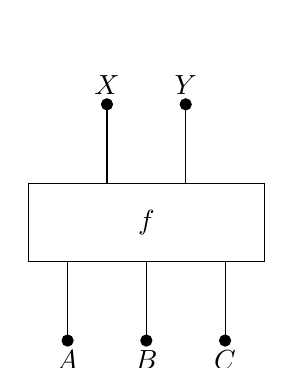
\begin{tikzpicture}
    \filldraw[black] (-0.5,0) circle (2pt) node[anchor=south]{$X$};
    \filldraw[black] (0.5,0) circle (2pt) node[anchor=south]{$Y$};
    \draw (-0.5, 0) -- (-0.5, -1);
    \draw (0.5, 0) -- (0.5, -1);
    \draw (-1.5, -1) -- (-1.5, -2) -- (1.5, -2) -- (1.5, -1) -- cycle;
    \draw (-1, -2) -- (-1, -3);
    \draw (0, -2) -- (0, -3);
    \draw (1, -2) -- (1, -3);
    \draw (0,-1.5) node{$f$};
    \filldraw[black] (-1,-3) circle (2pt) node[anchor=north]{$A$};
    \filldraw[black] (0,-3) circle (2pt) node[anchor=north]{$B$};
    \filldraw[black] (1,-3) circle (2pt) node[anchor=north]{$C$};
  \end{tikzpicture}
\end{center}

We can compose morphisms by concatenating their diagrams.
\begin{center}
  \begin{tikzpicture}
    \filldraw[black] (-0.5,0) circle (2pt) node[anchor=south]{$X$};
    \filldraw[black] (0.5,0) circle (2pt) node[anchor=south]{$Y$};
    \draw (-0.5, 0) -- (-0.5, -1);
    \draw (0.5, 0) -- (0.5, -1);
    \draw (-1.5, -1) -- (-1.5, -2) -- (1.5, -2) -- (1.5, -1) -- cycle;
    \draw (-1, -2) -- (-1, -3);
    \draw (0, -2) -- (0, -3);
    \draw (1, -2) -- (1, -3);
    \draw (0,-1.5) node{$f$};
    \draw (-1.5, -4) -- (-1.5, -3) -- (1.5, -3) -- (1.5, -4) -- cycle;
    \draw (0,-3.5) node{$g$};
    \draw (0, -4) -- (0, -5);
    \filldraw[black] (0, -5) circle (2pt) node[anchor=north]{$Z$};
  \end{tikzpicture}
\end{center}

In a braided monoidal category, we require that for any two objects $X$ and $Y$ we have an isomorphism $\gamma_{XY}\colon X \otimes Y \to Y \otimes X$, which we draw like this.

\begin{center}
  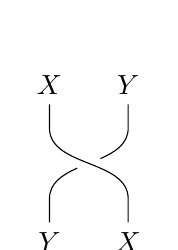
\begin{tikzpicture}
    \braid (braid) s_1;
    \node[at=(braid-1-s), anchor=south]{$X$};
    \node[at=(braid-2-s), anchor=south]{$Y$};
    \node[at=(braid-1-e), anchor=north]{$X$};
    \node[at=(braid-2-e), anchor=north]{$Y$};
  \end{tikzpicture}
\end{center}

Since $\gamma_{AB}$ is an isomorphism, it has an inverse $\gamma_{AB}^{-1}$ (not necessarily equal to $\gamma_{BA}$!) which we draw like this.

\begin{center}
  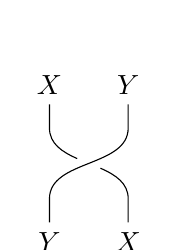
\begin{tikzpicture}
    \braid (braid) s_{1}^{-1};
    \node[at=(braid-1-s), anchor=south]{$X$};
    \node[at=(braid-2-s), anchor=south]{$Y$};
    \node[at=(braid-1-e), anchor=north]{$X$};
    \node[at=(braid-2-e), anchor=north]{$Y$};
  \end{tikzpicture}
\end{center}

The idea of a braided monoidal category is that we want to take these pictures seriously: we want two expressions involving repeated applications of the $\gamma_{\cdot\cdot}$ and their inverses to be equivalent if and only if the braid diagrams representing them are homotopic. Thus we want, for example,
\begin{equation*}
  \gamma_{XY} \circ \gamma_{YZ} \circ \gamma_{XY} =  \gamma_{YZ} \circ \gamma_{XY} \circ \gamma_{YZ}
\end{equation*}
since
\begin{equation*}
  \begin{aligned}
    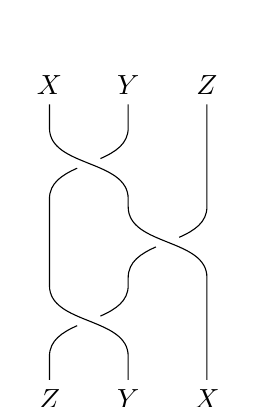
\begin{tikzpicture}
      \braid (braid) s_1 s_{2} s_{1};
      \node[at=(braid-1-s), anchor=south]{$X$};
      \node[at=(braid-2-s), anchor=south]{$Y$};
      \node[at=(braid-3-s), anchor=south]{$Z$};
      \node[at=(braid-1-e), anchor=north]{$X$};
      \node[at=(braid-2-e), anchor=north]{$Y$};
      \node[at=(braid-3-e), anchor=north]{$Z$};
    \end{tikzpicture}
  \end{aligned}
  \qquad\text{is homotopic to}\qquad
  \begin{aligned}
    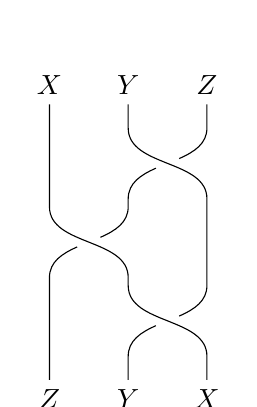
\begin{tikzpicture}
      \braid (braid) s_2 s_{1} s_{2};
      \node[at=(braid-1-s), anchor=south]{$X$};
      \node[at=(braid-2-s), anchor=south]{$Y$};
      \node[at=(braid-3-s), anchor=south]{$Z$};
      \node[at=(braid-1-e), anchor=north]{$X$};
      \node[at=(braid-2-e), anchor=north]{$Y$};
      \node[at=(braid-3-e), anchor=north]{$Z$};
    \end{tikzpicture}
  \end{aligned}
  .
\end{equation*}

A digression into the theory of braid groups would take us too far afield. The punchline is that to guarantee that all such compositions involving the $\gamma$ are identified in the correct way, we must define braided monoidal categories as follows.

\begin{definition}[braided monoidal category]\label{def:braidedmonoidalcategory}
  A catgory $\mathsf{C}$ with monoidal structure $(\otimes, 1, \alpha, \lambda, \rho)$ is \defn{braided} if for every two objects $A$ and $B \in \Obj(\mathsf{C})$, there is an isomorphism $\gamma_{A,B}\colon A \otimes B \to B \otimes A$ such that the following \emph{hexagon diagrams} commute.
  \begin{equation*}
    \begin{tikzcd}
      & A \otimes (B \otimes C) \arrow[r, "{\gamma_{A, B \otimes C}}"] & (B \otimes C) \otimes A \arrow[dr, "\alpha_{BCA}"] & \\
      (A \otimes B) \otimes C \arrow[ur, "\alpha_{ABC}"] \arrow[dr, swap, "\gamma_{AB} \otimes 1"] & & & B \otimes (C \otimes A) \\
      & (B \otimes A) \otimes C \arrow[r, swap, "\alpha_{BAC}"] & B \otimes (A \otimes C) \arrow[ur, swap, "1 \otimes \gamma"]
    \end{tikzcd}
  \end{equation*}
  \begin{equation*}
    \begin{tikzcd}
      & (A \otimes B) \otimes C \arrow[r, "{\gamma_{A \otimes B, C}}"] & C \otimes (A \otimes B) \arrow[dr, "\alpha^{-1}_{CAB}"] \\
      A \otimes (B \otimes C) \arrow[ur, "\alpha_{ABC}^{-1}"] \arrow[dr, swap, "1 \otimes \gamma_{BC}"] & & & (C \otimes A) \otimes B \\
      & A \otimes (C \otimes B) \arrow[r, swap, "\alpha^{-1}_{ACB}"] & (A \otimes C) \otimes B \arrow[ur, swap, "\gamma_{AC} \otimes 1"]
    \end{tikzcd}
  \end{equation*}
  The collection of such $\gamma$ form a natural isomorphism betweem the bifunctors
  \begin{equation*}
    (A, B) \mapsto A \otimes B\qquad\text{and}\qquad (A,B) \mapsto B \otimes A,
  \end{equation*}
  and is called a \defn{braiding}.
\end{definition}

\begin{definition}[braided monoidal functor]\label{def:braidedmonoidalfunctor}
  A lax monoidal functor $(\mathcal{F}, \Phi, \phi)$ (\hyperref[def:monoidalfunctor]{Definition~\ref*{def:monoidalfunctor}}) is \defn{braided monoidal} if it makes the following diagram commute.
  \begin{equation*}
    \begin{tikzcd}[row sep=huge, column sep=huge]
      \mathcal{F}(x) \otimes \mathcal{F}(y)
      \arrow[r, "{\gamma_{\mathcal{F}(x), \mathcal{F}(y)}}"]
      \arrow[d, swap, "{\Phi_{x,  y}}"]
      & \mathcal{F}(y) \otimes \mathcal{F}(x)
      \arrow[d, "{\Phi_{x, y}}"]
      \\
      \mathcal{F}(x \otimes y)
      \arrow[r, "{\mathcal{F}(\gamma_{x, y})}"]
      & \mathcal{F}(y \otimes x)
    \end{tikzcd}
  \end{equation*}
  \begin{note}
    There are no extra conditions imposed on a monoidal natural transformation to turn it into a braided natural transformation.
  \end{note}
\end{definition}

\subsection{Symmetric monoidal categories}
Until now, we have been calling the bifunctor $\otimes$ in \hyperref[def:monoidalcategory]{Definition~\ref*{def:monoidalcategory}} a tensor product. This has been an abuse of terminology: in general, one defines tensor products not to be those bifunctors which come from any monoidal category, but only those which come from \emph{symmetric} monoidal categories. We will define these shortly.

Conceptually, passing from the definition of a braided monoidal category to that of a symmetric monoidal category is rather simple. One only requires that for any two objects $A$ and $B$, $\gamma_{BA} = \gamma_{AB}^{-1}$, i.e. $\gamma_{BA} \circ \gamma_{AB} = 1_{A \otimes B}$.

We can interpret this nicely in terms of our braid diagrams. We can draw $\gamma_{BA} \circ \gamma_{AB}$ like this.

\begin{center}
  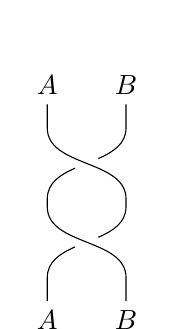
\begin{tikzpicture}
    \braid (braid) s_1 s_1;
    \node[at=(braid-1-s), anchor=south]{$A$};
    \node[at=(braid-2-s), anchor=south]{$B$};
    \node[at=(braid-1-e), anchor=north]{$A$};
    \node[at=(braid-2-e), anchor=north]{$B$};
  \end{tikzpicture}
\end{center}

The requirement that this must be homotopic to the identity transformation
\begin{center}
  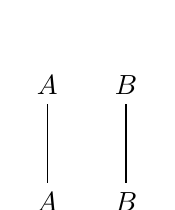
\begin{tikzpicture}
    \draw (0,0) node[anchor=south]{$A$} -- (0,-1) node[anchor=north]{$A$};
    \draw (1,0) node[anchor=south]{$B$} -- (1,-1) node[anchor=north]{$B$};
  \end{tikzpicture}
\end{center}

can be expressed by making the following rule: in a \emph{symmetric} monoidal category, we don't care about the difference between undercrossings and overcrossings:
\begin{equation*}
  \begin{aligned}
    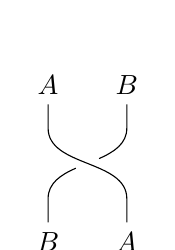
\begin{tikzpicture}
      \braid (braid) s_1;
      \node[at=(braid-1-s), anchor=south]{$A$};
      \node[at=(braid-2-s), anchor=south]{$B$};
      \node[at=(braid-1-e), anchor=north]{$A$};
      \node[at=(braid-2-e), anchor=north]{$B$};
    \end{tikzpicture}
  \end{aligned}
  \qquad = \qquad
  \begin{aligned}
    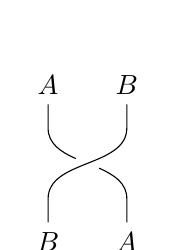
\begin{tikzpicture}
      \braid (braid) s_1^{-1};
      \node[at=(braid-1-s), anchor=south]{$A$};
      \node[at=(braid-2-s), anchor=south]{$B$};
      \node[at=(braid-1-e), anchor=north]{$A$};
      \node[at=(braid-2-e), anchor=north]{$B$};
    \end{tikzpicture}
  \end{aligned}
  .
\end{equation*}

Then we can exchange the diagram representing $\gamma_{BA} \circ \gamma_{AB}$ for

\begin{center}
  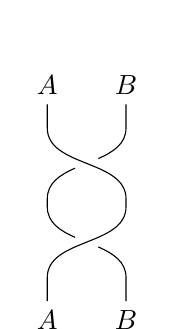
\begin{tikzpicture}
    \braid (braid) s_1 s_1^{-1};
    \node[at=(braid-1-s), anchor=south]{$A$};
    \node[at=(braid-2-s), anchor=south]{$B$};
    \node[at=(braid-1-e), anchor=north]{$A$};
    \node[at=(braid-2-e), anchor=north]{$B$};
  \end{tikzpicture}
\end{center}
which is clearly homotopic to the identity transformation on $A \otimes B$.

\begin{definition}[symmetric monoidal category]\label{def:symmetricmonoidalcategory}
  Let $\mathsf{C}$ be a braided monoidal category with braiding $\gamma$. We say that $\mathsf{C}$ is a \defn{symmetric monoidal category} if for all $A$, $B \in \Obj(\mathsf{C})$, $\gamma_{BA} \circ \gamma_{AB} = 1_{A \otimes B}$. A braiding $\gamma$ which satisfies such a condition is called \defn{symmetric}.
\end{definition}

\begin{note}
  There are no extra conditions imposed on a monoidal natural transformation to turn it into a symmetric natural transformation.
\end{note}

\section{Internal hom functors}\label{sec:internalhomfunctors}
We can now generalize the notion of an exponential object (\hyperref[def:exponential]{Definiton~\ref*{def:exponential}}) to any monoidal category.
\subsection{The internal hom functor}
Recall the definition of the hom functor on a locally small category $\mathsf{C}$ (\hyperref[def:homfunctor]{Definition~\ref*{def:homfunctor}}): it is the functor which maps two objects to the set of morphisms between them, so it is a functor
\begin{equation*}
  \mathsf{C}^{\mathrm{op}} \times \mathsf{C} \rightsquigarrow \mathsf{Set}.
\end{equation*}

If we take $\mathsf{C} = \mathsf{Set}$, then our hom functor never really leaves $\mathsf{Set}$; it is \emph{internal} to $\mathsf{Set}$. This is our first example of an \emph{internal hom functor}. In fact, it is the prototypical internal hom functor, and we can learn a lot by studying its properties.

Let $X$ and $Y$ be sets. Denote the set of all functions $X \to Y$ by $[X,Y]$.

Let $S$ be any other set, and consider a function $f\colon S \to [X, Y]$. For each element $s \in S$, $f$ picks out a function $h_{s}\colon X \to Y$. But this is just a curried version of a function $S \times X \to Y$! So as we saw in \hyperref[section:homfunctor]{Section~\ref*{section:homfunctor}}, we have a bijection between the sets $[S, [X, Y]]$ and $[S \times X, Y]$. In fact, this is even a \emph{natural} bijection, i.e.\ a natural transformation between the functors
\begin{equation*}
  [-,[-,-]]\qquad \text{and}\quad [- \times -, -]\colon \mathsf{Set}^{\mathrm{op}} \times \mathsf{Set}^{\mathrm{op}} \times \mathsf{Set} \rightsquigarrow \mathsf{Set}.
\end{equation*}

Let's check this. First, we need to figure out how our functors act on functions. Suppose we have sets and functions like so.
\begin{equation*}
  \begin{tikzcd}[row sep=tiny]
    A''
    & B''
    \arrow[l, swap, "f''"]
    \\
    A'
    & B'
    \arrow[l, swap, "f'"]
    \\
    A
    \arrow[r, "f"]
    & B
  \end{tikzcd}
\end{equation*}
Our functor maps
\begin{equation*}
  (A'', A', A) \mapsto [A'', [A', A]] = \Hom_{\mathsf{Set}}(A'', \Hom_{\mathsf{Set}}(A', A)),
\end{equation*}
so it should map $(f'', f', f)$ to a function
\begin{equation*}
  [f'', [f', f]]\colon [A'', [A', A]] \to [B'', [B', B]].
\end{equation*}
The way to do that is by sending $m \in [A'', [A', A]]$ to
\begin{equation*}
  [f', f] \circ m \circ f''.
\end{equation*}
You can check that this works as advertised.

The other one's not so tough. Our functor maps an object $(A'', A', A)$ to $[A'' \times A', A]$. We need to map $(f'', f', f)$ to a function
\begin{equation*}
  [f'' \times f' , f]\colon [A'' \times A', A] \to [B'' \times B', B].
\end{equation*}
We do that by sending $m \in [A'' \times A', A]$ to
\begin{equation*}
  f \circ m \circ (f'', f') \in [B'' \times B', B].
\end{equation*}

Checking that $[-,[-,-]]$ and $[-\times-, -]$ really \emph{are} functorial would be a bit much; each is just the composition of hom functor and the Cartesian product. We will however check that there is a natural isomorphism between them, which amounts to checking that the following diagram commutes.
\begin{equation*}
  \begin{tikzcd}[column sep=0.9]
    {[A'' \times A', A]}
    \arrow[rrr, "{[f'' \times f', f]}"]
    \arrow[ddd, swap, "{\Phi_{[A'' \times A', A]}}"]
    & & & {[B'' \times B', B]}
    \arrow[ddd, "{\Phi_{[B'' \times B', B]}}"]
    \\
    & m
    \arrow[d, mapsto]
    \arrow[r, mapsto]
    & f \circ m \circ (f', f'')
    \arrow[d, mapsto]
    \\
    & \Phi(m)
    \arrow[r, mapsto]
    & {[f', f] \circ \Phi(m) \circ f'' \stackrel{!}{=} \Phi(f \circ m \circ (f', f''))}
    \\
    {[A'', [A', A]]}
    \arrow[rrr, swap, "{[f'', [f', f]]}"]
    & & & {[B'', [B', B]]}
  \end{tikzcd}
\end{equation*}
In other words, we have to show that
\begin{equation*}
  \Phi_{[A'' \times A', A]}(f \circ m \circ (f', f'')) = [f', f] \circ \Phi_{[B'' \times B', B]}(m) \circ f''.
\end{equation*}

So what is each of these? Well, $f \circ m \circ (f', f'')$ is a map $B'' \times B' \to B$, which maps (say) $(b'', b') \mapsto b$.

The natural transformation $\Phi$ tells us to curry this, i.e.\ turn it into a map $B'' \to [B', B]$. Not just any map, though: a map which when evaluated on $b''$ turns into a map which, when evaluated on $b'$, yields $b$.

We know that $f \circ m \circ (f', f'')\colon (b'', b') \mapsto b$, i.e.
\begin{equation*}
  f(m(f''(b''), f'(b'))) = b.
\end{equation*}
If we can show that this is \emph{also} what $[f', f] \circ \Phi_{[B'' \times B', B]}(m) \circ f''$ is equal to when evaluated on $b''$ and then $b'$, we are done, since two functions are equal if they take the same value for all inputs.

Well, let's go through what this definition means. First, we take $b''$ and feed it to $f''$. Next, we let $\Phi_{[B'' \times B', B]}(m)$ act on the result, i.e.\ we fill the first argument of $m$ with $f''(b'')$. What we get is the following:
\begin{equation*}
  m(f''(b''), -).
\end{equation*}
Then we are to precompose this with $f'$ and stick the result into $f$:
\begin{equation*}
  f(m(f''(b''), f'(-))).
\end{equation*}
Finally, we are to evaluate this on $b'$ to get
\begin{equation*}
  f(m(f''(b''), f'(b'))).
\end{equation*}

Indeed, this is equal to $b$, so the diagram commutes.

In other words, $\Phi$ is a natural bijection between the hom-sets $[-,[-,-]]$ and $[- \times -, -]$.

We picked this example because the collection $[A, B]$ of all functions between two sets $A$ and $B$ is itself a set. Therefore it makes sense to think of the hom-sets $\Hom_{\mathsf{C}}(A, B)$ as living within the same category as $A$ and $B$. We saw in \hyperref[sec:cartesianclosedcategories]{Section~\ref*{sec:cartesianclosedcategories}} that in a category with products, we could sometimes view hom-sets as exponential objects. However, we now have the technology to be even more general.

\begin{definition}[internal hom functor]\label{def:internalhomfunctor}
  Let $(\mathsf{C}, \otimes)$ be a monoidal category. An \defn{internal hom functor} is a functor
  \begin{equation*}
    {[-, -]}_{\mathsf{C}}\colon \mathsf{C}^{\mathrm{op}} \times \mathsf{C} \rightsquigarrow \mathsf{C}
  \end{equation*}
  such that for every $X \in \Obj(\mathsf{C})$ we have a pair of adjoint functors
  \begin{equation*}
    (-) \otimes X \dashv {[X, -]}_{\mathsf{C}}.
  \end{equation*}

  The objects ${[A, B]}_{\mathsf{C}}$ are called \defn{internal hom objects}.
\end{definition}

\begin{note}
  The reason for the long introduction to this section was that the pair of adjoint functors in \hyperref[def:internalhomfunctor]{Definition~\ref*{def:internalhomfunctor}} really matches the one in $\mathsf{Set}$. Recall, in $\mathsf{Set}$ there was a natural transformation
  \begin{equation*}
    \Hom_{\mathsf{Set}}(S \times X, Y) \simeq \Hom_{\mathsf{Set}}(S, [X, Y]).
  \end{equation*}

  This means that for any set $X$, there is a pair of adjoint functors
  \begin{equation*}
    (-) \times X \dashv [X, -],
  \end{equation*}
  which is in agreement with the statement of \hyperref[def:internalhomfunctor]{Definition~\ref*{def:internalhomfunctor}}.
\end{note}

\begin{notation}
  The convention at the nLab is to denote the internal hom by square braces $[A,B]$, and this is for the most part what we will do. Unfortunately, we have already used this notation for the \emph{regular} hom functor. To remedy this, we will add a subscript if the category to which the hom functor belongs is not clear: ${[-,-]}_{\mathsf{C}}$ for a hom functor internal to $\mathsf{C}$, ${[-,-]}_{\mathsf{Set}}$ for the standard hom functor (or the hom functor internal to $\mathsf{Set}$, which amounts to the same).

  There is no universally accepted notation for the internal hom functor. One often sees it denoted by a lower-case $\hom$: $\hom_{\mathsf{C}}(A, B)$. Many sources (for example DMOS~\cite{DMOS}) distinguish the internal hom with an underline: $\underline{\Hom}_{\mathsf{C}}(A, B)$. Deligne typesets it with a script H\@: $\mathscr{H}om_{\mathsf{C}}(A, B)$.
\end{notation}

\begin{definition}[closed monoidal category]\label{def:closedmonoidalcategory}
  A monoidal category equipped with an internal hom functor is called a \defn{closed monoidal category}.
\end{definition}

\begin{note}
  Here is another (clearly equivalent) definition of ${[X, Y]}_{\mathsf{C}}$: it is the object representing (\hyperref[def:representablefunctor]{Definition~\ref*{def:representablefunctor}}) the functor
  \begin{equation*}
    T \mapsto \Hom_\mathsf{C}(T \otimes X, Y).
  \end{equation*}
\end{note}

\begin{example}
  In many locally small categories whose objects can be thought of as ``sets with extra structure,'' it is possible to pile structure on top of the hom sets until they themselves can be viewed as bona fide objects in their categories. It often (\emph{but not always!}) happens that these beefed-up hom sets coincide (up to isomorphism) with the internal hom objects.

  Take for example $\mathsf{Vect}_{k}$. For any vector spaces $V$ and $W$, we can turn $\Hom_{\mathsf{Vect}_{k}}(V, W)$ into a vector space by defining addition and scalar multiplication pointwise; we can then view $\Hom_{\mathsf{Vect}_{k}}(V, W)$ as belonging to $\Obj(\mathsf{Vect}_{k})$. It turns out that this is precisely (up to isomorphism) the internal hom object ${[V, W]}_{\mathsf{Vect}_{k}}$.

  To see this, we need to show that there is a natural bijection
  \begin{equation*}
    \Hom_{\mathsf{Vect}_{k}}(A, \Hom_{\mathsf{Vect}_{k}}(B, C)) \simeq \Hom_{\mathsf{Vect}_{k}}(A \otimes B, C).
  \end{equation*}

  Suppose we are given a linear map $f\colon A \to \Hom_{\mathsf{Vect}_{k}}(B, C)$. If we act with this on an element of $A$, we get a linear map $B \to C$. If we evaluate this on an element of $B$, we get an element of $C$. Thus, we can view $f$ as a bilinear map $A \times B \to C$, hence as a linear map $A \otimes B \to C$.

  Now suppose we are given a linear map $g\colon A \otimes B \to C$. By pre-composing this with the tensor product we can view this as a bilinear map $A \times B \to C$, and by currying this we get a linear map $A \to \Hom_{\mathsf{Vect}_{k}}(B, C)$.
\end{example}

For the remainder of this chapter, let $(\mathsf{C}, \otimes, 1)$ be a closed monoidal category with internal hom functor ${[-,-]}_{\mathsf{C}}$.

In a closed monoidal category, the adjunction between the internal hom and the tensor product even holds internally.
\begin{lemma}
  For any $X$, $Y$, $Z \in \Obj(\mathsf{C})$ there is a natural isomorphism
  \begin{equation*}
    {[X \otimes Y, Z]}_{\mathsf{C}} \stackrel{\sim}{\to} {[X, {[Y, Z]}_{\mathsf{C}}]}_{\mathsf{C}}.
  \end{equation*}
\end{lemma}
\begin{proof}
  Let $A \in \Obj(\mathsf{C})$. We have the following string of natural isomorphisms.
  \begin{align*}
    \Hom_{\mathsf{C}}(A, {[X \otimes Y, Z]}_{\mathsf{C}}) &\simeq \Hom_{\mathsf{C}}(A \otimes (X \otimes Y), Z) \\
    &\simeq \Hom_{\mathsf{C}}((A \otimes X) \otimes Y, Z) \\
    &\simeq \Hom_{\mathsf{C}}(A \otimes X, {[Y, Z]}_{\mathsf{C}}) \\
    &\simeq \Hom_{\mathsf{C}}(A, {[X, {[Y, Z]}_{\mathsf{C}}]}_{\mathsf{C}}).
  \end{align*}

  Since this is true for each $A$ we have, by \hyperref[cor:yonedaembeddingrespectsisomorphisms]{Corollary~\ref*{cor:yonedaembeddingrespectsisomorphisms}},
  \begin{equation*}
    {[X \otimes Y, Z]}_{\mathsf{C}} \stackrel{\sim}{\to} {[X, {[Y, Z]}_{\mathsf{C}}]}_{\mathsf{C}}.
  \end{equation*}
\end{proof}

\begin{lemma}\label{lemma:cantensorbothsidesofinternalhom}
  Let $(\mathsf{C}, \otimes, 1)$ be a closed symmetric monoidal category. For any $A$, $B$, $R \in \Obj(\mathsf{C})$, there is a natural transformation
  \begin{equation*}
    {[A, B]}_{\mathsf{C}} \to {[R \otimes A, R \otimes B]}_{\mathsf{C}},
  \end{equation*}
  natural in $A$ and $B$.
\end{lemma}
\begin{proof}
  The assignment $R \otimes (-)$ is a functor, and induces a transformation of the regular hom functor
  \begin{equation*}
    \Hom_{\mathsf{C}}(A, B) \mapsto \Hom_{\mathsf{C}}(R \otimes A, R \otimes B)
  \end{equation*}
  which is natural in $A$ and $B$. We would like to show that the internal hom functor also has this property.

  The following string of natural transformations guarantees it by the Yoneda lemma.
  \begin{align*}
    \Hom_{\mathsf{C}}(X, {[A, B]}_{\mathsf{C}}) &\simeq \Hom_{\mathsf{C}}(X \otimes A, \otimes B) \\
    &\simeq \Hom_{\mathsf{C}}(R \otimes X \otimes A, R \otimes B) \\
    &\simeq \Hom_{\mathsf{C}}(X \otimes (R \otimes A), R \otimes B) \\
    & \simeq \Hom_{\mathsf{C}}(X, {[R \otimes A, R \otimes B]}_{\mathsf{C}}).
  \end{align*}
\end{proof}

\subsection{The evaluation map}
The internal hom functor gives us a way to talk about evaluating morphisms $f\colon X \to Y$ without mentioning elements of $X$.
\begin{definition}[evaluation map]\label{def:evaluationmap}
  Let $X \in \Obj(\mathsf{C})$. We have seen that the adjunction
  \begin{equation*}
    (-) \otimes X \dashv {[X, -]}_{\mathsf{C}}
  \end{equation*}
  gives us, for any $A$, $X$, $Y \in \Obj(\mathsf{C})$, a natural bijection
  \begin{equation*}
    \Hom_{\mathsf{C}}(A \otimes X, Y) \overset{\sim}{\to} \Hom_{\mathsf{C}}(A, {[X, Y]}_{\mathsf{C}}).
  \end{equation*}
  In particular, with $A = {[X, Y]}_{\mathsf{C}}$, we have a bijection
  \begin{equation*}
    \Hom_{\mathsf{C}}({[X, Y]}_{\mathsf{C}} \otimes X, Y) \overset{\sim}{\to} \Hom_{\mathsf{C}}({[X, Y]}_{\mathsf{C}}, {[X, Y]}_{\mathsf{C}}).
  \end{equation*}

  The adjunct (\hyperref[def:adjunct]{Definition~\ref*{def:adjunct}}) of $1_{{[X, Y]}_{\mathsf{C}}} \in \Hom_{\mathsf{C}}({[X, Y]}_{\mathsf{C}}, {[X, Y]}_{\mathsf{C}})$ is an object in $\Hom_{\mathsf{C}}\left( {[X, Y]}_{\mathsf{C}} \otimes X, Y \right)$, denoted
  \begin{equation*}
    \ev_{X, Y}\colon {[X, Y]}_{\mathsf{C}} \otimes X \to Y,
  \end{equation*}
  and called the \defn{evaluation map}.
\end{definition}

\begin{example}\label{eg:evaluationmapinset}
  As we saw in \hyperref[eg:setisamonoidalcategory]{Example~\ref*{eg:setisamonoidalcategory}}, the category $\mathsf{Set}$ is a monoidal category with a bifunctor given by the cartesian product. The internal hom is simply the regular hom functor
  \begin{equation*}
    \Hom_{\mathsf{Set}}(-,-) = [-,-].
  \end{equation*}
  Let us explore the evaluation map on $\mathsf{Set}$. It is the adjunct of the identity map $1_{[X, Y]}$ under the adjunction
  \begin{equation*}
    [[X, Y] \times X, Y] \dashv [[X, Y], [X, Y]].
  \end{equation*}
  Thus, it is a function
  \begin{equation*}
    \ev_{X, Y}\colon [X, Y] \times X \to Y;\qquad (f, x) \mapsto \ev_{X, Y}(f, x).
  \end{equation*}
  So far, we don't know what $\ev_{X, Y}$ sends $(f, x)$ to; we just know that we'd \emph{like it} if it sent it to $f(x)$.

  The above adjunction is given by currying: we start on the LHS with a map $\ev_{X, Y}$ with two arguments, and we turn it into a map which fills in only the first argument. Thus the map on the RHS adjunct to $\ev_{X, Y}$ is given by
  \begin{equation*}
    f \mapsto \ev_{X, Y}(f, -).
  \end{equation*}
  If we want the map $f \mapsto \ev_{X, Y}(f, -)$ to be the identity map, $f$ and $\ev_{X, Y}(f, -)$ must agree on all elements $x$, i.e.
  \begin{equation*}
    f(x) = \ev_{X, Y}(f, x)\qquad\text{for all }x \in X.
  \end{equation*}
  Thus, the evaluation map is the map which sends $(f, x) \mapsto f(x)$.
\end{example}

\subsection{The composition morphism}
The evaluation map allows us to define composition of morphisms without talking about internal hom objects as if they have elements.
\begin{definition}[composition morphism]\label{def:compositionmorphism}
  For $X$, $Y$, $Z \in \Obj(\mathsf{C})$, the \defn{composition morphism}
  \begin{equation*}
    \circ_{X, Y, Z}\colon {[Y, Z]}_{\mathsf{C}} \otimes {[X, Y]}_{\mathsf{C}} \to {[X, Z]}_{\mathsf{C}}
  \end{equation*}
  is the $(-) \otimes X \vdash {[X, -]}_{\mathsf{C}}$-adjunct of the composition
  \begin{equation*}
    \begin{tikzcd}[column sep=huge]
      {[Y, Z]}_{\mathsf{C}} \otimes {[X, Y]}_{\mathsf{C}} \otimes X
      \arrow[r, "{\left(1_{{[Y, Z]}_{\mathsf{C}}}, \ev_{X, Y}\right)}"]
      & {{[Y, Z]}_{\mathsf{C}}} \otimes Y
      \arrow[r, "{\ev_{Y, Z}}"]
      & Z
    \end{tikzcd}.
  \end{equation*}
\end{definition}

\begin{example}
  In $\mathsf{Set}$, the composition morphism $\circ_{X, Y, Z}$ lives up to its name. Let $f\colon X \to Y$, $g\colon Y \to Z$, and $x \in X$. The above composition goes as follows.
  \begin{enumerate}
    \item The map $\left( 1_{[Y, Z]}, \ev_{X, Y} \right)$ turns the triple $(g, f, x)$ into the pair $(g, f(x))$.

    \item The map $\ev_{Y, Z}$ turns $(g, f(x))$ into $g(f(x)) = (g \circ f)(x)$.
  \end{enumerate}

  The evaluation morphism $\circ_{X, Y, Z}$ is the currying of this, i.e.\ it sends
  \begin{equation*}
    (f, g) \mapsto (f \circ g)(-).
  \end{equation*}
\end{example}

\subsection{Dual objects}
Recall that for any $k$-vector space $V$, there is a dual vector space
\begin{equation*}
  V^{*} = \left\{ L\colon V \to k \right\}.
\end{equation*}
This definition generalizes to any closed monoidal category.

\begin{definition}[dual object]\label{def:dualobject}
  Let $X \in \Obj(\mathsf{C})$. The \defn{dual object} to $X$, denoted $X^{*}$, is defined to be the object
  \begin{equation*}
    {[X, 1]}_{\mathsf{C}}.
  \end{equation*}

  That is to say, $X^{*}$ is the internal hom object modelling the hom set of morphisms from $X$ to the identity object $1$.
\end{definition}

\begin{notation}
  The evaluation morphism (\hyperref[def:evaluationmap]{Definition~\ref*{def:evaluationmap}}) has a component
  \begin{equation*}
    \ev_{X^{*}, X}\colon X^{*} \otimes X \to 1.
  \end{equation*}

  To clean things up a bit, we will write $\ev_{X}$ instead of $\ev_{X^{*}, X}$.
\end{notation}

\begin{notation}
  In many sources, e.g. DMOS (\cite{DMOS}), the dual object to $X$ is denoted $X^{\vee}$ instead of $X^{*}$.
\end{notation}

\begin{lemma}
  There is a natural isomorphism between the functors
  \begin{equation*}
    \Hom_{\mathsf{C}}(-, X^{*})\qquad\text{and}\qquad \Hom_{\mathsf{C}}((-) \otimes X, 1).
  \end{equation*}
\end{lemma}
\begin{proof}
  For any $X$, $T \in \Obj(\mathsf{C})$, the definition of the internal hom ${[-,-]}_{\mathsf{C}}$ gives us a natural isomorphism
  \begin{equation*}
    \Hom_{\mathsf{C}}(T \otimes X, 1) \simeq \Hom_{\mathsf{C}}(T, {[X, 1]}_{\mathsf{C}}) = \Hom_{\mathsf{C}}(T, X^{*}).
  \end{equation*}
\end{proof}

\begin{theorem}
  The map $X \mapsto X^{*}$ can be extended to a contravariant functor.
\end{theorem}
\begin{proof}
  We need to figure out how our functor should act on morphisms. We define this by analogy with the familiar setting of vector spaces. Recall that for a linear map $L\colon V \to W$, the dual map $L^{t}\colon W^{*} \to V^{*}$ is defined by
  \begin{equation*}
    (L^{t}(w))(v) = w(L(v)).
  \end{equation*}

  By analogy, for $f \in \Hom_{\mathsf{C}}(X, Y)$, we should define the dual morphism $f^{t} \in \Hom_{\mathsf{C}}(B^{*}, A^{*})$ by demanding that the following diagram commutes.
  \begin{equation*}
    \begin{tikzcd}[row sep=huge, column sep=huge]
      h^{*} \otimes X
      \arrow[r, "f^{t} \otimes 1_{X}"]
      \arrow[d, swap, "1_{Y} \otimes f"]
      & X^{*} \otimes X
      \arrow[d, "\ev_{X}"]
      \\
      h^{*} \otimes Y
      \arrow[r, "\ev_{Y}"]
      & 1
    \end{tikzcd}
  \end{equation*}

  To check that this is functorial, we must check that it respects compositions, i.e.\ that the following diagram commutes.
  \begin{equation*}
    \begin{tikzcd}[row sep=huge, column sep=huge]
      Z^{*} \otimes X
      \arrow[r, "(f^{t} \circ g^{t}) \otimes 1_{X}"]
      \arrow[d, swap, "1_{Z} \otimes (g \circ f)"]
      & X^{*} \otimes X
      \arrow[d, "\ev_{X}"]
      \\
      Z^{*} \otimes Z
      \arrow[r, "\ev_{Z}"]
      & 1
    \end{tikzcd}
  \end{equation*}

  Let's add in some more objects and morphisms.
  \begin{equation*}
    \begin{tikzcd}[row sep=huge, column sep=huge]
      Z^{*} \otimes X
      \arrow[r, "g^{t} \otimes 1_{X}"]
      \arrow[d, swap, "1_{Z^{*}} \otimes f"]
      & h^{*} \otimes X
      \arrow[r, "f^{t} \otimes 1_{X}"]
      \arrow[d, swap, "1_{h^{*}} \otimes f"]
      & X^{*} \otimes X
      \arrow[dd, "\ev_{X}"]
      \\
      Z^{*} \otimes Y
      \arrow[r, "g^{t} \otimes 1_{Y}"]
      \arrow[d, swap, "1_{Z^{*}} \otimes g"]
      & h^{*} \otimes Y
      \arrow[dr, "\ev_{Y}"]
      \\
      Z^{*} \otimes Z
      \arrow[rr, swap, "\ev_{Z}"]
      & & 1
    \end{tikzcd}
  \end{equation*}

  We want to show that the outer square commutes. But it clearly does: that the top left square commutes is trivial, and the right and bottom `squares' are the commutativity conditions defining $f^{t}$ and $g^{t}$.
\end{proof}

\begin{note}
  It's not clear to me why $f^{t}$ as defined above exists and is unique.
\end{note}

The above is one, but not the only, way to define dual objects. We can be more general.
\begin{definition}[right duality]\label{def:rightduality}
  Let $\mathsf{C}$ be a category with monoidal structure $(\otimes, 1, \alpha, \lambda, \rho)$. \defn{Right duality} of two objects $A$ and $A^{*} \in \Obj(\mathsf{C})$ consists of
  \begin{enumerate}
    \item A morphism of the form
      \begin{equation*}
        \ev_{A}\colon A^{*} \otimes A \to 1,
      \end{equation*}
      called the \emph{evaluation map} (or \emph{counit} if you're into Hopf algebras)

    \item A morphism of the form
      \begin{equation*}
        i_{A}\colon 1 \to A \otimes A^{*},
      \end{equation*}
      called the \emph{coevaluation} map (or \emph{unit})
  \end{enumerate}
  such that the compositions
  \begin{equation*}
    \begin{tikzcd}[column sep=huge]
      X
      \arrow[r, "i_{A} \otimes 1_{X}"]
      & (X \otimes X^{*}) \otimes X
      \arrow[r, "{\alpha_{X, X^{*}, X}}"]
      & X \otimes (X^{*} \otimes X)
      \arrow[r, "{1_{X} \otimes \ev_{X}}"]
      & X
      \\
      X^{*}
      \arrow[r, "{1_{X^{*}} \otimes \ev_{X}}"]
      & X^{*} \otimes (X \otimes X^{*})
      \arrow[r, "{\alpha^{-1}_{X^{*}, X, X^{*}}}"]
      & (X^{*} \otimes X) \otimes X^{*}
      \arrow[r, "{\ev_{X}\otimes 1_{X^{*}}}"]
      & X^{*}
    \end{tikzcd}
  \end{equation*}
  are the identity morphism.
\end{definition}

\begin{definition}[rigid monoidal category]\label{def:rigidmonoidalcategory}
  A monoidal category $(\mathsf{C}, \otimes, 1)$ is \defn{rigid} if every object has a left and right dual.
\end{definition}

\begin{theorem}
  Every rigid monoidal category is a closed monoidal category (i.e.\ has an internal hom functor, see \hyperref[def:closedmonoidalcategory]{Definition~\ref*{def:closedmonoidalcategory}}) with internal hom object
  \begin{equation*}
    {[A, B]}_{\mathsf{C}} \simeq B \otimes A^{*}.
  \end{equation*}
\end{theorem}
\begin{proof}
  We can prove the existence of this isomorphism by showing, thanks to \hyperref[cor:yonedaembeddingrespectsisomorphisms]{Corollary~\ref*{cor:yonedaembeddingrespectsisomorphisms}}, that for any $X \in \Obj(\mathsf{C})$ there is an isomorphsm
  \begin{equation*}
    \Hom_{\mathsf{C}}(X, {[A, B]}_{\mathsf{C}}) \simeq \Hom_{\mathsf{C}}(X, B \otimes A^{*}).
  \end{equation*}

  The defining adjunction of the internal hom gives us
  \begin{equation*}
    \Hom_{\mathsf{C}}(X, {[A, B]}_{\mathsf{C}}) \simeq \Hom_{\mathsf{C}}(X \otimes A, B).
  \end{equation*}

  Now we can map any $f \in \Hom_{\mathsf{C}}(X \otimes A, B)$ to
  \begin{equation*}
    (f \otimes 1_{A}) \circ (1_{X} \otimes i_{A}) \in \Hom_{\mathsf{C}}(X, B \otimes A^{*}).
  \end{equation*}

  We will be done if we can show that the assignment
  \begin{equation*}
    f \mapsto (f \otimes 1_{A}) \circ (1_{X} \otimes i_{A})
  \end{equation*}
  is an isomorphism. We'll do this by exhibiting an inverse:
  \begin{equation*}
    \Hom_{\mathsf{C}}(X, B \otimes A^{*}) \ni g \mapsto (1_{W} \otimes \ev_{V}) \circ (g \otimes 1_{V}) \in \Hom_{\mathsf{C}}(X \otimes A, B).
  \end{equation*}

  Of course, first we should show that $(f \otimes 1_{A}) \circ (1_{X} \otimes i_{A})$ really does map $X \to B \otimes A^{*}$. But it does; it does this by first acting on $X$ with $i_{A}$:
  \begin{equation*}
    X \to X \otimes A \otimes A^{*}
  \end{equation*}
  and then acting on the $X \otimes A$ with $f$ and letting the $A^{*}$ hang around:
  \begin{equation*}
    X \otimes A \otimes A^{*} \to B \otimes A^{*}.
  \end{equation*}

  To show that
  \begin{equation*}
    g \mapsto (1_{B} \otimes \ev_{A}) \circ (g \otimes 1_{A})
  \end{equation*}
  really is an inverse, we can shove the assignment
  \begin{equation*}
    f \mapsto (f \otimes 1_{A}) \circ (1_{X} \otimes i_{A})
  \end{equation*}
  into it and show that we get $f$ right back out. That is to say, we need to show that
  \begin{equation*}
    (1_{B} \otimes \ev_{A}) \circ (\left[ (f \otimes 1_{A}) \circ (1_{X} \otimes i_{A}) \right] \otimes 1_{A}) = f.
  \end{equation*}
  This is easy to see but hard to type. Write it out. You'll need to use first of the two composition identities.

  To show that the other composition yields $g$, you have to use the other.
\end{proof}

\chapter{Abelian categories}\label{sec:abeliancategories}
This section draws heavily from~\cite{EGNO-tensor-categories}.
\section{Additive categories}
Recall that $\mathsf{Ab}$ is the category of abelian groups.
\begin{definition}[$\mathsf{Ab}$-enriched category]\label{def:abenrichedcategory}
  A category $\mathsf{C}$ is \defn{$\mathsf{Ab}$-enriched} if
  \begin{enumerate}
    \item for all objects $A$, $B \in \Obj(\mathsf{C})$, the hom-set $\text{Hom}_{\mathsf{C}}(A, B)$ has the structure of an abelian group (i.e.\ one can add morphisms), such that

    \item the composition
      \begin{equation*}
        \circ\colon \Hom_{\mathsf{C}}(B, C) \times \Hom_{\mathsf{C}}(A, B) \to \Hom_{C}(A, C)
      \end{equation*}
      is additive in each slot: for any $f_{1}$, $f_{2} \in \Hom_{\mathsf{C}}(B, C)$ and $g \in \Hom_{\mathsf{C}}(A, B)$, we must have
      \begin{equation*}
        (f_{1} + f_{2}) \circ g = f_{1} \circ g + f_{2} \circ g,
      \end{equation*}
      and similarly in the second slot.
  \end{enumerate}
\end{definition}

\begin{note}\label{note:inabenrichedcategorynoemptyhomsets}
  In any $\mathsf{Ab}$-enriched category, every hom-set has at least one element---the identity element of the hom-set taken as an abelian group.
\end{note}

\begin{definition}[endomorphism ring]\label{def:endomorphismring}
  Let $\mathsf{C}$ be an $\mathsf{Ab}$-enriched category, and let $A \in \Obj(\mathsf{C})$. The \defn{endomorphism ring} of $A$, denoted $\mathrm{End}(A)$, is $\Hom_{\mathsf{C}}(A, A)$, with addition given by the abelian structure and multiplication given by composition.
\end{definition}

\begin{lemma}\label{lemma:abeliancategorycoproductsareproducts}
  In an $\mathsf{Ab}$-enriched category $\mathsf{C}$, a finite product is also a coproduct, and vice versa. In particular, initial objects and terminal objects coincide.
\end{lemma}
\begin{proof}
  %First, we show that initial and terminal objects coincide. Let $\emptyset$ be initial and $*$ terminal in $\mathsf{C}$.
  %
  %Since $\Hom_{\mathsf{C}}(\emptyset, \emptyset)$ has only one element, it must be both the identity morphism on $\emptyset$ \emph{and} the identity element of $\Hom_{\mathsf{C}}(\emptyset, \emptyset)$ as an abelian group. Similarly, $1_{*}$ must be the identity element of $\Hom_{\mathsf{C}}(*, *)$.

  %Since $\emptyset$ is initial and $*$ is final, $\Hom_{\mathsf{C}}(\emptyset, *)$ has exactly one element $f$. By \hyperref[note:inabenrichedcategorynoemptyhomsets]{Note \ref*{note:inabenrichedcategorynoemptyhomsets}}, we are guaranteed that $\Hom_{\mathsf{C}}(*, \emptyset)$ has at least one element.

  See~\cite{nlab-additive-category}, Proposition 2.1 for details.
\end{proof}

\begin{definition}[additive category]\label{def:additivecategory}
  A category $\mathsf{C}$ is \defn{additive} if it has biproducts (\hyperref[def:categorywithbiproducts]{Definition~\ref*{def:categorywithbiproducts}}) and is $\mathsf{Ab}$-enriched.
\end{definition}


\begin{example}
  The category $\mathsf{Ab}$ of Abelian groups is an additive category. We have already seen that it has the direct sum $\oplus$ as biproduct. Given any two abelian groups $A$ and $B$ and morphisms $f$, $g\colon A \to B$, we can define the sum $f + g$ via
  \begin{equation*}
    (f + g)(a) = f(a) + g(a)\qquad\text{for all }a \in A.
  \end{equation*}
  Then for another abelian group $C$ and a morphism $h\colon B \to C$, we have
  \begin{equation*}
    \left[ h \circ (f+g) \right](a) = h(f(a) + g(a)) = h(f(a)) + h(g(a)) = \left[ h \circ f + h \circ g \right](a),
  \end{equation*}
  so
  \begin{equation*}
    h \circ (f+g) =h \circ f + h \circ g,
  \end{equation*}
  and similarly in the other slot.
\end{example}

\begin{example}
  The category $\mathsf{Vect}_{k}$ is additive. Since vector spaces are in particular abelian groups under addition, it is naturally $\mathsf{Ab}$-enriched,
\end{example}

\begin{definition}[additive functor]\label{def:additivefunctor}
  Let $\mathcal{F}\colon \mathsf{C} \rightsquigarrow \mathsf{D}$ be a functor between additive categories. We say that $\mathcal{F}$ is \defn{additive} if for each $X$, $Y \in \Obj(\mathsf{C})$ the map
  \begin{equation*}
    \Hom_{\mathsf{C}}(X, Y) \to \Hom_{\mathsf{D}}(\mathcal{F}(X), \mathcal{F}(Y))
  \end{equation*}
  is a homomorphism of abelian groups.
\end{definition}

\begin{lemma}
  For any additive functor $\mathcal{F}\colon \mathsf{C} \rightsquigarrow \mathsf{D}$, there exists a natural isomorphism
  \begin{equation*}
    \Phi\colon \mathcal{F}(-) \oplus \mathcal{F}(-) \Rightarrow \mathcal{F}(- \oplus -).
  \end{equation*}
\end{lemma}
\begin{proof}
  The commutativity of the following diagram is immediate.
  \begin{equation*}
    \begin{tikzcd}[column sep=huge, row sep=huge]
      \mathcal{F}(X \oplus Y)
      \arrow[r, "\mathcal{F}(f \oplus g)"]
      \arrow[d, swap, "\Phi_{X, Y}"]
      & \mathcal{F}(X' \oplus Y')
      \arrow[d, "\Phi_{X', Y'}"]
      \\
      \mathcal{F}(X) \oplus \mathcal{F}(Y)
      \arrow[r, "\mathcal{F}(f) \oplus \mathcal{F}(g)"]
      & \mathcal{F}(X') \oplus \mathcal{F}(Y')
    \end{tikzcd}
  \end{equation*}

  The $(X, Y)$-component $\Phi_{X, Y}$ is an isomorphism because
\end{proof}

\section{Pre-abelian categories}~\label{sec:preabeliancategories}
\begin{definition}[pre-abelian category]\label{def:preabeliancategory}
  A category  $\mathsf{C}$ is \defn{pre-abelian} if it is additive and every morphism has a kernel (\hyperref[def:kernelofmorphism]{Definition~\ref*{def:kernelofmorphism}}) and a cokernel (\hyperref[def:cokernalofmorphism]{Definition~\ref*{def:cokernalofmorphism}}).
\end{definition}

\begin{lemma}\label{lemma:preabeliancategorieshaveequalizers}
  Pre-abelian categories have equalizers (\hyperref[def:equalizer]{Definition~\ref*{def:equalizer}}).
\end{lemma}
\begin{proof}
  We show that in an pre-abelian category, the equalizer of $f$ and $g$ coincides with the kernel of $f - g$. It suffices to show that the kernel of $f - g$ satisfies the universal property for the equalizer of $f$ and $g$.

  Here is the diagram for the universal property of the kernel of $f - g$.
  \begin{equation*}
    \begin{tikzcd}
      Z
      \arrow[rrd, bend left]
      \arrow[ddr, bend right, swap, "i"]
      \arrow[dr, dashed, "\exists!\bar{\imath}"]
      \\
      & \ker(f - g)
      \arrow[d, swap, "\iota_{f - g}"]
      \arrow[r]
      & 0
      \arrow[d]
      \\
      & A
      \arrow[r, "f - g"]
      & B
    \end{tikzcd}
  \end{equation*}

  The universal property tells us that for any object $Z \in \Obj(\mathsf{C})$ and any morphism $i\colon Z \to A$ with $i \circ (f - g) = 0$ (i.e. $i \circ f = i \circ g$), there exists a unique morphism $\bar{\imath}\colon Z \to \ker(f - g)$ such that $i = \bar{\imath} \circ \iota_{f - g}$.
\end{proof}

\begin{corollary}
  Every pre-abelian category has all finite limits.
\end{corollary}
\begin{proof}
  By \hyperref[thm:criterionforfinitelimits]{Theorem~\ref*{thm:criterionforfinitelimits}}, a category has finite limits if and only if it has finite products and equalizers. Pre-abelian categories have finite products by definition, and equalizers by \hyperref[lemma:preabeliancategorieshaveequalizers]{Lemma~\ref*{lemma:preabeliancategorieshaveequalizers}}.
\end{proof}

Recall from \hyperref[sec:biproducts]{Section~\ref*{sec:biproducts}} the following definition.

\begin{definition}[zero morphism]\label{def:zeromorphism}
  Let $\mathsf{C}$ be a category with zero object $0$. For any two objects $A$, $B \in \Obj(\mathsf{C})$, the \defn{zero morphism} $0_{A,B}$ is the unique morphism $A \to B$ which factors through $0$.
  \begin{equation*}
    \begin{tikzcd}
      A
      \arrow[rr, bend left, "0_{A, B}"]
      \arrow[r]
      & 0
      \arrow[r]
      & B
    \end{tikzcd}
  \end{equation*}
\end{definition}

\begin{notation}
  It will often be clear what the source and destination of the zero morphism are; in this case we will drop the subscripts, writing $0$ instead of $0_{AB}$.
\end{notation}

It is easy to see that the left- or right-composition of the zero morphism with any other morphism results in the zero morphism: $f \circ 0 = 0$ and $0 \circ g = 0$.

\begin{lemma}\label{lemma:everymorphisminapreabeliancategoryfactors}
  Every morphism $f\colon A \to B$ in a pre-abelian catgory has a canonical decomposition
  \begin{equation*}
    \begin{tikzcd}
      A
      \arrow[r, "p"]
      & \coker(\ker(f))
      \arrow[r, "\bar{f}"]
      & \ker(\coker(f))
      \arrow[r, "i"]
      & B
    \end{tikzcd},
  \end{equation*}
  where $p$ is an epimorphism (\hyperref[def:epimorphism]{Definition~\ref*{def:epimorphism}}) and $i$ is a monomorphism (\hyperref[def:monomorphism]{Definition~\ref*{def:monomorphism}}).
\end{lemma}
\begin{proof}
  We start with a map
  \begin{equation*}
    \begin{tikzcd}
      A
      \arrow[r, "f"]
      & B
    \end{tikzcd}.
  \end{equation*}

  Since we are in a pre-abelian category, we are guaranteed that $f$ has a kernel $(\ker(f), \iota)$ and a cokernel $(\coker(f), \pi)$. From the universality squares it is immediate that $f \circ \iota = 0$ and $\pi \circ f = 0$ This tells us that the composition $\pi \circ f \circ \iota = 0$, so the following commutes.
  \begin{equation*}
    \begin{tikzcd}
      & A
      \arrow[r, "f"]
      & B
      \arrow[dr, "\pi"]
      \\
      \ker(f)
      \arrow[ur, "\iota"]
      \arrow[dr]
      & & & \coker(f)
      \\
      & 0
      \arrow[r]
      & 0
      \arrow[ur]
    \end{tikzcd}
  \end{equation*}
  We know that $\pi$ has a kernel $(\ker(\pi), i)$ and $\iota$ has a cokernel $(\coker(\iota), p)$, so we can add their commutativity squares as well.
  \begin{equation*}
    \begin{tikzcd}
      & A
      \arrow[r, "f"]
      \arrow[d, "p"]
      & B
      \arrow[dr, "\pi"]
      \\
      \ker(f)
      \arrow[ur, "\iota"]
      \arrow[dr]
      & \coker(\iota)
      & \ker(\pi)
      \arrow[u, "i"]
      \arrow[d]
      & \coker(f)
      \\
      & 0
      \arrow[u]
      \arrow[r]
      & 0
      \arrow[ur]
    \end{tikzcd}
  \end{equation*}

  If we squint hard enough, we can see the following diagram.
  \begin{equation*}
    \begin{tikzcd}
      A
      \arrow[rrd, bend left]
      \arrow[rdd, bend right, swap, "f"]
      \\
      & \ker(\pi)
      \arrow[r]
      \arrow[d, "i"]
      & 0
      \arrow[d]
      \\
      & B
      \arrow[r, "\pi"]
      & \coker(f)
    \end{tikzcd}
  \end{equation*}
  The outer square commutes because $\pi \circ f = 0$, so the universal property for $\ker(\pi)$ gives us a unique morphism $A \to \ker(\pi)$. Let's add this to our diagram, along with a morphism $0 \to \ker(\pi)$ which trivially keeps everything commutative.
  \begin{equation*}
    \begin{tikzcd}
      & A
      \arrow[r, "f"]
      \arrow[d, "p"]
      \arrow[dr]
      & B
      \arrow[dr, "\pi"]
      \\
      \ker(f)
      \arrow[ur, "\iota"]
      \arrow[dr]
      & \coker(\iota)
      & \ker(\pi)
      \arrow[u, "i"]
      \arrow[d]
      & \coker(f)
      \\
      & 0
      \arrow[u]
      \arrow[r]
      \arrow[ur]
      & 0
      \arrow[ur]
    \end{tikzcd}
  \end{equation*}

  Again, buried in the bowels of our new diagram, we find the following.
  \begin{equation*}
    \begin{tikzcd}
      \ker(f)
      \arrow[r, "\iota"]
      \arrow[d]
      & A
      \arrow[d, "\pi"]
      \arrow[ddr, bend left]
      \\
      0
      \arrow[r]
      \arrow[drr, bend right]
      & \coker(\iota)
      \\
      & & \ker(\pi)
    \end{tikzcd}
  \end{equation*}
  And again, the universal property of cokernels gives us a unique morphism $\bar{f}\colon \coker(\iota) \to \ker(\pi)$.
  \begin{equation*}
    \begin{tikzcd}
      & A
      \arrow[r, "f"]
      \arrow[d, "p"]
      \arrow[dr]
      & B
      \arrow[dr, "\pi"]
      \\
      \ker(f)
      \arrow[ur, "\iota"]
      \arrow[dr]
      & \coker(\iota)
      \arrow[r, "\bar{f}"]
      & \ker(\pi)
      \arrow[u, "i"]
      \arrow[d]
      & \coker(f)
      \\
      & 0
      \arrow[u]
      \arrow[r]
      \arrow[ur]
      & 0
      \arrow[ur]
    \end{tikzcd}
  \end{equation*}

  The fruit of our laborious construction is the following commuting square.
  \begin{equation*}
    \begin{tikzcd}
      A
      \arrow[r, "f"]
      \arrow[d, swap, "p"]
      & B
      \arrow[d, "i"]
      \\
      \coker(\iota)
      \arrow[r, "\bar{f}"]
      & \ker(\pi)
    \end{tikzcd}
  \end{equation*}
  We have seen (\hyperref[lemma:canonicalinjectionismono]{Lemma~\ref*{lemma:canonicalinjectionismono}}) that $i$ is mono, and (\hyperref[lemma:canonicalsurjectionisepi]{Lemma~\ref*{lemma:canonicalsurjectionisepi}}) that $p$ is epi.

  Now we abuse terminology by calling $\iota = \ker(f)$ and $\pi = \coker(f)$. Then we have the required decomposition.
\end{proof}

\begin{note}
  The abuse of notation above is ubiquitous in the literature.
\end{note}

\section{Abelian categories}
This section is under very heavy construction. Don't trust anything you read here.
\begin{definition}[abelian category]\label{def:abeliancategory}
  A pre-abelian category $\mathsf{C}$ is \defn{abelian} if for each morphism $f$, the canonical morphism guaranteed by \hyperref[lemma:everymorphisminapreabeliancategoryfactors]{Lemma~\ref*{lemma:everymorphisminapreabeliancategoryfactors}}
  \begin{equation*}
    \bar{f}\colon \coker(\ker(f)) \to \ker(\coker(f))
  \end{equation*}
  is an isomorphism.
\end{definition}

\begin{note}
  The above piecemeal definition is equivalent to the following.

  A category $\mathsf{C}$ is \emph{abelian} if
  \begin{enumerate}
    \item it is $\mathsf{Ab}$-enriched \hyperref[def:additivecategory]{Definition~\ref*{def:additivecategory}}, i.e.\ each hom-set has the structure of an abelian group and composition is bilinear;
    \item it admits finite coproducts, hence (by \hyperref[lemma:abeliancategorycoproductsareproducts]{Lemma~\ref*{lemma:abeliancategorycoproductsareproducts}}) biproducts and zero objects;
    \item every morphism has a kernel and a cokernel;
    \item for every morphism, $f$, the canonical morphism $\bar{f}\colon \coker(\ker(f)) \to \ker(\coker(f))$ is an isomorphism.
  \end{enumerate}
\end{note}

For the remainder of the section, let $\mathsf{C}$ be an abelian category.

\begin{lemma}
  In an abelian category, every morphism decomposes into the composition of an epimorphism and a monomorphism.
\end{lemma}
\begin{proof}
  For any morphism $f$, bracketing the decomposition $f = i \circ \bar{f} \circ p$ as
  \begin{equation*}
    i \circ (\bar{f} \circ p).
  \end{equation*}
  gives such a composition.
\end{proof}

\begin{note}
  The above decomposition is unique up to unique isomorphism.
\end{note}

\begin{definition}[image of a morphism]\label{def:imageofamorphism}
  Let $f\colon A \to B$ be a morphism. The object $\ker(\coker(f))$ is called the \defn{image} of $f$, and is denoted $\im(f)$.
\end{definition}

\begin{lemma}\label{lemma:morphismwhichkillsontherightismono}
  $\,$
  \begin{enumerate}
    \item A morphism $f\colon A \to B$ is mono iff for all $Z \in \Obj(\mathsf{C})$ and for all $g\colon Z \to A$, $f \circ g = 0$ implies $g = 0$.
    \item A morphism $f\colon A \to B$ is epi iff for all $Z \in \Obj(\mathsf{C})$ and for all $g\colon B \to Z$, $g \circ f = 0$ implies $g = 0$.
  \end{enumerate}
\end{lemma}
\begin{proof}
  $\,$
  \begin{enumerate}
    \item First, suppose $f$ is mono. Consider the following diagram.
      \begin{equation*}
        \begin{tikzcd}
          Z
          \arrow[r, shift left, "g"]
          \arrow[r, swap, shift right, "0"]
          & A
          \arrow[r, "f"]
          & B
        \end{tikzcd}
      \end{equation*}

      If the above diagram commutes, i.e.\ if $f \circ g = 0$, then $g = 0$, so $1 \implies 2$.

      Now suppose that for all $Z \in \Obj(\mathsf{C})$ and all $g\colon Z \to A$, $f \circ g = 0$ implies $g = 0$.

      Let $g$, $g'\colon Z \to A$, and suppose that $f \circ g = f \circ g'$. Then $f \circ (g - g') = 0$. But that means that $g - g' = 0$, i.e. $g = g'$. Thus, $2 \implies 1$.

    \item Dual to the proof above.
  \end{enumerate}
\end{proof}

\begin{lemma}\label{lemma:monoifkernelzeroepiifcokerzero}
  Let $f\colon A \to B$. We have the following.
  \begin{enumerate}
    \item The morphism $f$ is mono iff $\ker(f) = 0$\label{part:monoifkernelzeroepiifcokerzero1}
    \item The morphism $f$ is epi iff $\coker(f) = 0$.\label{part:monoifkernelzeroepiifcokerzero2}
  \end{enumerate}
\end{lemma}
\begin{proof}
  $\,$
  \begin{enumerate}
    \item We first show that if $\ker(f) = 0$, then $f$ is mono. Suppose $\ker(f) = 0$. By the universal property of kernels, we know that for any $Z \in \Obj(\mathsf{C})$ and any $g\colon Z \to A$ with $f \circ g = 0$ there exists a unique map $\bar{g}\colon Z \to \ker(f)$ such that $g = \iota \circ \bar{g}$.
      \begin{equation*}
        \begin{tikzcd}
          Z
          \arrow[rdd, bend right, swap, "g"]
          \arrow[rd, dashed, "\exists!g"]
          \\
          & \ker(f) = 0
          \arrow[r]
          \arrow[d, swap, "\iota"]
          & 0
          \arrow[d]
          \\
          & A
          \arrow[r, "f"]
          & B
        \end{tikzcd}
      \end{equation*}
      But then $g$ factors through the zero object, so we must have $g = 0$. This shows that $f \circ g = 0 \implies g = 0$, and by \hyperref[lemma:morphismwhichkillsontherightismono]{Lemma~\ref*{lemma:morphismwhichkillsontherightismono}} $f$ must be mono.

      Next, we show that if $f$ is mono, then $\ker(f) = 0$. To do this, it suffices to show that $\ker(f)$ is final, i.e.\ that there exists a unique morphism from every object to $\ker(f)$.

      Since $\Hom_{\mathsf{C}}(Z, \ker(f))$ has the structure of an abelian group, it must contain at least one element. Suppose it contains two morphisms $h_{1}$ and $h_{2}$.
      \begin{equation*}
        \begin{tikzcd}
          Z
          \arrow[rd, shift left, "h_{1}"]
          \arrow[rd, shift right, swap, "h_{2}"]
          \\
          & \ker(f)
          \arrow[r]
          \arrow[d, swap, "\iota"]
          & 0
          \arrow[d]
          \\
          & A
          \arrow[r, "f"]
          & B
        \end{tikzcd}
      \end{equation*}
      Our aim is to show that $h_{1} = h_{2}$. To this end, compose each with $\iota$.
      \begin{equation*}
        \begin{tikzcd}
          Z
          \arrow[rd, shift left, "h_{1}"]
          \arrow[rd, shift right, swap, "h_{2}"]
          \arrow[rdd, bend right, shift left, "\iota \circ h_{1}"]
          \arrow[rdd, bend right, shift right, swap, "\iota \circ h_{2}"]
          \\
          & \ker(f)
          \arrow[r]
          \arrow[d, swap, "\iota"]
          & 0
          \arrow[d]
          \\
          & A
          \arrow[r, "f"]
          & B
        \end{tikzcd}
      \end{equation*}
      Since $f \circ \iota = 0$, we have $f \circ (\iota \circ h_{1}) = 0$ and $f \circ (\iota \circ h_{2}) = 0$. But since $f$ is mono, by \hyperref[lemma:morphismwhichkillsontherightismono]{Lemma~\ref*{lemma:morphismwhichkillsontherightismono}}, we must have $\iota \circ h_{1} = 0 = \iota \circ h_{2}$. But by \hyperref[lemma:canonicalinjectionismono]{Lemma~\ref*{lemma:canonicalinjectionismono}}, $\iota$ is mono, so again we have
      \begin{equation*}
        h_{1} = h_{2} = 0,
      \end{equation*}
      and we are done.

    \item Dual to the proof above.
  \end{enumerate}
\end{proof}

\begin{lemma}
  We have the following.
  \begin{enumerate}
    \item The kernel of the zero morphism $0: A \to B$ is the pair $(A, 1_{A})$.
    \item The cokernel of the zero morphism $0: A \to B$ is the pair $(B, 1_{B})$.
  \end{enumerate}
\end{lemma}
\begin{proof}
  $\,$
  \begin{enumerate}
    \item We need only verify that the universal property is satisfied. That is, for any object $Z \in \Obj(\mathsf{C})$ and any morphism $h\colon Z \to A$ such that $0 \circ g = 0$, there exists a unique morphism $\bar{g}\colon Z \to \ker(0)$ such that the following diagram commutes.
      \begin{equation*}
        \begin{tikzcd}
          Z
          \arrow[rdd, swap, bend right, "g"]
          \arrow[rd, dashed, "\bar{g}=g"]
          \\
          & \ker(0) = A
          \arrow[r, "0"]
          \arrow[d, swap, "\iota = 1_{A}"]
          & 0
          \arrow[d]
          \\
          & A
          \arrow[r, "0"]
          & B
        \end{tikzcd}
      \end{equation*}
      But this is pretty trivial: $\bar{g} = g$.

    \item Dual to above.
  \end{enumerate}
\end{proof}

\begin{theorem}
  All abelian categories are binormal (\hyperref[def:binormalcategory]{Definition~\ref*{def:binormalcategory}}). That is to say:
  \begin{enumerate}
    \item all monomorphisms are kernels
    \item all epimorphisms are cokernels.
  \end{enumerate}
\end{theorem}
\begin{proof}
  $\,$
  \begin{enumerate}
    \item Consider the following diagram taken \hyperref[lemma:everymorphisminapreabeliancategoryfactors]{Lemma~\ref*{lemma:everymorphisminapreabeliancategoryfactors}}, which shows the canonical factorization of any morphism $f$.
      \begin{equation*}
        \begin{tikzcd}
          & A
          \arrow[r, "f"]
          \arrow[d, "p"]
          \arrow[dr]
          & B
          \arrow[dr, "\pi"]
          \\
          \ker(f)
          \arrow[ur, "\iota"]
          \arrow[dr]
          & \coker(\iota)
          \arrow[r, "\bar{f}"]
          & \ker(\pi)
          \arrow[u, "i"]
          \arrow[d]
          & \coker(f)
          \\
          & 0
          \arrow[u]
          \arrow[r]
          \arrow[ur]
          & 0
          \arrow[ur]
        \end{tikzcd}
      \end{equation*}

      By definition of a pre-abelian category, we know that $\bar{f}$ is an isomorphism.
  \end{enumerate}
\end{proof}

\begin{note}
  The above theorem is actually an equivalent definition of an abelian category, but the proof of equivalence is far from trivial. See e.g.~\cite{freyd-abelian-categories} for details.
\end{note}

\begin{definition}[subobject, quotient object, subquotient object]\label{def:subobjectquotientobject}
  Let $Y \in \Obj(\mathsf{C})$.
  \begin{enumerate}
    \item A \defn{subobject} of $Y$ is an object $X \in \Obj(\mathsf{C})$ together with a monomorphism $i\colon X \hookrightarrow Y$. If $X$ is a subobject of $Y$ we will write $X \subseteq Y$.
    \item A \defn{quotient object} of $Y$ is an object $Z$ together with an epimorphism $p\colon Y \twoheadrightarrow Z$.
    \item A \defn{subquotient object} of $Y$ is a quotient object of a subobject of $Y$.
  \end{enumerate}
\end{definition}

%\begin{lemma}
%  Let $O$ be an object, $Z$ be a subquotient of $O$, and $Z'$ a subquotient of $Z$. Then $Z'$ is a subquotient of $O$.
%\end{lemma}
%\begin{proof}
%  A subquotient $Z$ of $O$ is a quotient $Z$ of a subobject $X$ of $O$.
%  \begin{equation*}
%    \begin{tikzcd}
%      X
%      \arrow[r, hookrightarrow]
%      \arrow[d, twoheadrightarrow]
%      & O
%      \\
%      Z
%    \end{tikzcd}
%  \end{equation*}
%  A subquotient $Z'$ of $Z$ looks like this.
%  \begin{equation*}
%    \begin{tikzcd}
%      & X
%      \arrow[r, hookrightarrow]
%      \arrow[d, twoheadrightarrow]
%      & O
%      \\
%      X'
%      \arrow[r, hookrightarrow]
%      \arrow[d, twoheadrightarrow]
%      & Z
%      \\
%      Z'
%    \end{tikzcd}
%  \end{equation*}
%
%  Take pullback yadda yadda. Will finish later.
%\end{proof}

\begin{definition}[quotient]\label{def:quotient}
  Let $X \subseteq Y$, i.e.\ let there exist a monomorphism $f\colon X \hookrightarrow Y$. The \defn{quotient} $Y/X$ is the cokernel $(\coker(f), \pi_{f})$.
\end{definition}

\begin{example}
  Let $V$ be a vector space, $W \subseteq V$ a subspace. Then we have the canonical inclusion map $\iota\colon W \hookrightarrow V$, so $W$ is a subobject of $V$ in the sense of \hyperref[def:subobjectquotientobject]{Definition~\ref*{def:subobjectquotientobject}}.

  According to \hyperref[def:quotient]{Definition~\ref*{def:quotient}}, the quotient $V / W$ is the cokernel $(\coker(\iota), \pi_{\iota})$ of $\iota$. We saw in \hyperref[eg:invectcokernelsarequotientsbyimage]{Example~\ref*{eg:invectcokernelsarequotientsbyimage}} that the cokernel of $\iota$ was $V / \im(\iota)$. However, $\im(\iota)$ is exactly $W$! So the categorical notion of the quotient $V / W$ agrees with the linear algebra notion.
\end{example}

\begin{definition}[$k$-linear category]\label{def:linearcategory}
  An abelian category \hyperref[def:abeliancategory]{Definition~\ref*{def:abeliancategory}} $\mathsf{C}$ is \defn{$k$-linear} if for all $A$, $B \in \Obj(\mathsf{C})$ the hom-set $\Hom_{\mathsf{C}}(A, B)$ has the structure of a $k$-vector space whose additive structure is the abelian structure, and for which the composition of morphisms is $k$-linear.
\end{definition}

\begin{example}
  The category $\mathsf{Vect}_{k}$ is $k$-linear.
\end{example}

\begin{definition}[$k$-linear functor]
  \label{def:linearfunctor}
  let $\mathsf{C}$ and $\mathsf{D}$ be two $k$-linear categories, and $\mathcal{F}\colon \mathsf{C} \rightsquigarrow \mathsf{D}$ a functor. Suppose that for all objects $C$, $D \in \Obj(\mathsf{C})$ all morphisms $f$, $g\colon C \to D$, and all $\alpha$, $\beta \in k$, we have
  \begin{equation*}
    \mathcal{F}(\alpha f + \beta g) = \alpha \mathcal{F}(f) + \beta \mathcal{G}(g).
  \end{equation*}

  Then we say that $\mathcal{F}$ is \defn{$k$-linear}.
\end{definition}

\section{Exact sequences}
\begin{definition}[exact sequence]
  \label{def:exactsequence}
  A sequence of morphisms
  \begin{equation*}
    \begin{tikzcd}
      \cdots
      \arrow[r]
      & X_{i-1}
      \arrow[r, "f_{i-1}"]
      & X_{i}
      \arrow[r, "f_{i}"]
      & X_{i+1}
      \arrow[r]
      & \cdots
    \end{tikzcd}
  \end{equation*}
  is called \defn{exact in degree $i$} if the image (\hyperref[def:imageofamorphism]{Definition \ref*{def:imageofamorphism}}) of $f_{i-1}$ is equal to the kernel (\hyperref[def:kernelofmorphism]{Definition \ref*{def:kernelofmorphism}}) of $f_{i}$. A sequence is \defn{exact} if it is exact in every degree.
\end{definition}

\begin{lemma}
  If a sequence
  \begin{equation*}
    \begin{tikzcd}
      \cdots
      \arrow[r]
      & X_{i-1}
      \arrow[r, "f_{i-1}"]
      & X_{i}
      \arrow[r, "f_{i}"]
      & X_{i+1}
      \arrow[r]
      & \cdots
    \end{tikzcd}
  \end{equation*}
  is exact in degree $i$, then $f_{i} \circ f_{i-1} = 0$.
\end{lemma}

\begin{definition}[short exact sequence]
  \label{def:shortexactsequence}
  A \defn{short exact sequence} is an exact sequence of the following form.
  \begin{equation*}
    \begin{tikzcd}
      0
      \arrow[r]
      & X
      \arrow[r]
      & Y
      \arrow[r]
      & Z
      \arrow[r]
      & 0
    \end{tikzcd}
  \end{equation*}
\end{definition}

%This definition has some immediate trivial consequences.
%\begin{lemma}
%  Let
%  \begin{equation*}
%    \begin{tikzcd}
%      0
%      \arrow[r]
%      & X
%      \arrow[r, "f"]
%      & Y
%      \arrow[r, "g"]
%      & Z
%      \arrow[r]
%      & 0
%    \end{tikzcd}
%  \end{equation*}
%  be a short exact sequence. Then
%  \begin{enumerate}
%    \item $f$ is mono
%    \item $g$ is epi
%    \item $Z \simeq Y/X$.
%  \end{enumerate}
%\end{lemma}
%\begin{proof}
%  $\,$
%  \begin{enumerate}
%    \item An easy consequence of \hyperref[lemma:monoifkernelzeroepiifcokerzero]{Lemma \ref*{lemma:monoifkernelzeroepiifcokerzero}, part \ref*{part:monoifkernelzeroepiifcokerzero1}}.
%    \item An easy consequence of \hyperref[lemma:monoifkernelzeroepiifcokerzero]{Lemma \ref*{lemma:monoifkernelzeroepiifcokerzero}, part \ref*{part:monoifkernelzeroepiifcokerzero2}}.
%    \item We need to show that
%  \end{enumerate}
%\end{proof}

\begin{definition}[exact functor]
  \label{def:exactfunctor}
  Let $\mathsf{C}$, $\mathsf{D}$ be abelian categories, $\mathcal{F}\colon \mathsf{C} \rightsquigarrow \mathsf{D}$ a functor. We say that $\mathcal{F}$ is
  \begin{itemize}
    \item \defn{left exact} if it preserves biproducts and kernels
    \item \defn{right exact} if it preserves biproducts and cokernels
    \item \defn{exact} if it is both left exact and right exact.
  \end{itemize}
\end{definition}

%\begin{theorem}
%  Let $\mathcal{F}\colon \mathsf{C} \rightsquigarrow \mathsf{D}$ be a functor between abelian categories. Let
%  \begin{equation*}
%    \begin{tikzcd}
%      0
%      \arrow[r]
%      & A
%      \arrow[r]
%      & B
%      \arrow[r]
%      & C
%      \arrow[r]
%      & 0
%    \end{tikzcd}
%  \end{equation*}
%  be a short exact sequence in $\mathsf{C}$. Then
%  \begin{itemize}
%    \item if $\mathcal{F}$ is left exact, then
%      \begin{equation*}
%        \begin{tikzcd}
%          0
%          \arrow[r]
%          & \mathcal{F}(A)
%          \arrow[r]
%          & \mathcal{F}(B)
%          \arrow[r]
%          & \mathcal{F}(C)
%        \end{tikzcd}
%      \end{equation*}
%      is an exact sequence in $\mathsf{D}$.
%
%    \item if $\mathcal{F}$ is right exact, then
%      \begin{equation*}
%        \begin{tikzcd}
%          \mathcal{F}(A)
%          \arrow[r]
%          & \mathcal{F}(B)
%          \arrow[r]
%          & \mathcal{F}(C)
%          \arrow[r]
%          & 0
%        \end{tikzcd}
%      \end{equation*}
%      is an exact sequence in $\mathsf{D}$.
%    \item if $\mathcal{F}$ is exact, then
%      \begin{equation*}
%        \begin{tikzcd}
%          0
%          \arrow[r]
%          & \mathcal{F}(A)
%          \arrow[r]
%          & \mathcal{F}(B)
%          \arrow[r]
%          & \mathcal{F}(C)
%          \arrow[r]
%          & 0
%        \end{tikzcd}
%      \end{equation*}
%      is an exact sequence in $\mathsf{D}$.
%  \end{itemize}
%\end{theorem}
%\begin{proof}
%
%\end{proof}

\section{Length of objects}
\begin{definition}[simple object]\label{def:simpleobject}A nonzero object $X \in \Obj(\mathsf{C})$ is called \defn{simple} if $0$ and $X$ are its only subobjects.
\end{definition}

\begin{example}
  In $\mathsf{Vect}_{k}$, the only simple object (up to isomorphism) is $k$, taken as a one-dimensional vector space over itself.
\end{example}

\begin{definition}[semisimple object]\label{def:semisimpleobject}
  An object $Y \in \Obj(\mathsf{C})$ is \defn{semisimple} if it is isomorphic to a dirct sum of simple objects.
\end{definition}

\begin{example}
  In $\mathsf{Vect}_{k}$, all finite-dimensional vector spaces are semisimple.
\end{example}

\begin{definition}[semisimple category]\label{def:semisimple category}
  An abelian category $\mathsf{C}$ is \defn{semisimple} if every object of $\mathsf{C}$ is semisimple.
\end{definition}

\begin{example}
  The category $\mathsf{FinVect}_{k}$ is semisimple.
\end{example}

\begin{definition}[Jordan-H{\"o}lder series]\label{def:jordanholderseries}
  Let $X \in \Obj(\mathsf{C})$. A filtration
  \begin{equation*}
    0 = X_{0} \subset X_{1} \subset \cdots \subset X_{n-1} \subset X_{n} = X
  \end{equation*}
  of $X$ such that $X_{i} / X_{i-1}$ is simple for all $i$ is called a \defn{Jordan H{\"o}lder series} for $X$. The integer $n$ is called the \defn{length} of the series $X_{i}$.
\end{definition}

The importance of Jordan-H{\"o}lder series is the following.

\begin{theorem}[Jordan-H{\"o}lder]\label{thm:jordanholdertheorem}
  Let $X_{i}$ and $Y_{i}$ be two Jordan-H{\"o}lder series for some object $X \in \Obj(\mathsf{C})$. Then the length of $X_{i}$ is equal to the length of $Y_{i}$, and the objects $Y_{i}/Y_{i-1}$ are a reordering of $X_{i}/X_{i-1}$.
\end{theorem}
\begin{proof}
  See~\cite{EGNO-tensor-categories}, pg. 5, Theorem 1.5.4.
\end{proof}

\begin{definition}[length]\label{def:length}
  The \defn{length} of an object $X$ is defined to be the length of any of its Jordan-H{\"o}lder series. This is well-defined by \hyperref[thm:jordanholdertheorem]{Theorem~\ref*{thm:jordanholdertheorem}}.
\end{definition}


\chapter{Tensor Categories}
The following definition is taken almost verbatim from~\cite{nlab-deligne-theorem}.
\begin{definition}[tensor category]\label{def:tensorcategory}
  Let $k$ be a field. A \defn{$k$-tensor category} $\mathsf{A}$ (as considered by Deligne in~\cite{deligne-categories-tensorielle}) is an
  \begin{enumerate}
    \item essentially small (\hyperref[def:essentiallysmall]{Definition~\ref*{def:essentiallysmall}})

    \item $k$-linear\footnote{Hence abelian.} (\hyperref[def:linearcategory]{Definition~\ref*{def:linearcategory}})

    \item rigid (\hyperref[def:rigidmonoidalcategory]{Definition~\ref*{def:rigidmonoidalcategory}})

    \item symmetric (\hyperref[def:symmetricmonoidalcategory]{Definition~\ref*{def:symmetricmonoidalcategory}})

    \item monoidal category (\hyperref[def:monoidalcategory]{Definition~\ref*{def:monoidalcategory}})
  \end{enumerate}
  such that
  \begin{enumerate}
    \item the tensor product functor $\otimes\colon \mathsf{A} \times \mathsf{A} \rightsquigarrow \mathsf{A}$ is, in both arguments separately,
      \begin{enumerate}
        \item $k$-linear (\hyperref[def:linearfunctor]{Definition~\ref*{def:linearfunctor}})

        \item exact (\hyperref[def:exactfunctor]{Definition~\ref*{def:exactfunctor}})
      \end{enumerate}

    \item $\mathrm{End}(1) \simeq k$, where $\mathrm{End}$ denotes the endomorphism ring (\hyperref[def:endomorphismring]{Definition~\ref*{def:endomorphismring}}).
  \end{enumerate}
\end{definition}

\begin{example}
  $\mathsf{Vect}_{k}$ is \emph{not} a tensor category because it is not essentially small; there is one isomorphism class of vector spaces for each cardinal, and there is no set of all cardinals. However, its subcategory $\mathsf{FinVect}_{k}$ is a tensor category.
\end{example}

\begin{definition}[finite tensor category]\label{def:finitetensorcategory}
  A $k$-tensor category $\mathsf{A}$ is called \defn{finite} (over $k$) if
  \begin{enumerate}
    \item There are only finitely many simple objects in $\mathsf{A}$, and each of them admits a projective presentation.

    \item Each object $A$ of $\mathsf{A}$ is of finite length.

    \item For any two objects $A$, $B$ of $\mathsf{A}$, the hom-object (i.e. $k$-vector space) $\Hom_{\mathsf{A}}(A, B)$ is finite-dimensional.
  \end{enumerate}
\end{definition}

\begin{example}
  The category $\mathsf{FinVect}_{k}$ is finite.
  \begin{enumerate}
    \item The only simple object is $k$ taken as a one-dimensional vector space over itself.

    \item The length of a finite-dimensional vector space is simply its dimension.

    \item The vector space $\Hom_{\mathsf{FinVect}}(V, W)$ has dimension $\dim(V) \dim(W)$.
  \end{enumerate}
\end{example}

\begin{definition}[finitely $\otimes$-generated]\label{def:finitelygenerated}
  A $k$-tensor category $\mathsf{A}$ is called \defn{finitely $\otimes$-generated} if there exists an object $E \in \Obj(\mathsf{A})$ such that every other object $X \in A$ is a subquotient (\hyperref[def:subobjectquotientobject]{Definition \ref*{def:subobjectquotientobject}}) of a finite direct sum of tensor products of $E$; that is to say, if there exists a finite collection of integers $n_{i}$ such that $X$ is a subquotient of $\bigoplus_{i} E^{\otimes^{n_{i}}}$.
  \begin{equation*}
    \begin{tikzcd}
      & \bigoplus_{i} E^{\otimes^{n_{i}}}
      \arrow[d, twoheadrightarrow, "\pi"]
      \\
      X
      \arrow[r, hookrightarrow, "\iota"]
      & \left( \bigoplus_{i} E^{\otimes^{n_{i}}} \right) / Q
    \end{tikzcd}
  \end{equation*}
\end{definition}

\begin{example}
  The category $\mathsf{FinVect}_{k}$ is finitely generated since any finite-dimensional vector space is isomorphic to $k^{n} = k \oplus \cdots \oplus k$ for some $n$.
\end{example}

\begin{definition}[subexponential growth]
  \label{def:subexponentialgrowth}
  A tensor category $\mathsf{A}$ has \defn{subexponential growth} if, for each object $X$ there exists a natural number $N_{X}$ such that
  \begin{equation*}
    \mathrm{len}(X^{\otimes_{n}}) \leq (N_{X})^{n}.
  \end{equation*}
\end{definition}

\begin{example}
  The category $\mathsf{FinVect}_{k}$ has subexponential growth. For any finite-dimensional vector space $V$, we always have
  \begin{equation*}
    \mathrm{dim}(V^{\otimes^{n}}) = (\dim(V))^{n},
  \end{equation*}
  so we can take $N_{V} = \mathrm{dim}(V)$.
\end{example}

\begin{theorem}
  Let $\mathsf{A}$ be a tensor category, and suppose that
  \begin{enumerate}
    \item every object $A \in \Obj(\mathsf{A})$ has a finite length

    \item the dimension of every hom space $\Hom_{\mathsf{A}}(A, B)$ is finite over $k$.
  \end{enumerate}

  Then the category $\mathsf{Ind}(\mathsf{A})$ of ind-objects of $\mathsf{A}$ (\hyperref[def:categoryofindobjects]{Definition \ref*{def:categoryofindobjects}}) has the following properties.
  \begin{enumerate}
    \item $\mathsf{Ind}(\mathsf{A})$ is abelian (\hyperref[def:abeliancategory]{Definition \ref*{def:abeliancategory}}).

    \item $A \hookrightarrow \mathsf{Ind}(\mathsf{A})$ is a full subcategory (cf. \hyperref[note:fullinclusionintoindcategory]{Note \ref*{note:fullinclusionintoindcategory}}).

    \item The tensor product on $\mathsf{A}$ extends to $\mathsf{Ind}(\mathsf{A})$ via
      \begin{align*}
        X \otimes Y &\simeq (\lim_{\rightarrow i}X_{i}) \otimes (\lim_{\rightarrow j}Y_{j}) \\
        &\simeq \lim_{\rightarrow i,j} (X_{i} \otimes Y_{j}).
      \end{align*}

    \item The category $\mathsf{Ind}(\mathsf{A})$ fails only to be a tensor category because it is not necessarily essentially small and rigid. More specifically, an object $A \in \mathsf{Ind}(\mathsf{A})$ is dualizable if and only if it is in $\mathsf{A}$.
  \end{enumerate}
\end{theorem}
\begin{proof}
  Proposition 3.38 in \cite{nlab-deligne-theorem}.
\end{proof}

\begin{definition}[tensor functor]
  \label{def:tensorfunctor}
  Let $(\mathscr{A}, \otimes_{A}, 1_{A})$ and $(\mathscr{B}, \otimes_{B}, 1_{B})$ be $k$-tensor categories. A functor $\mathcal{F}\colon \mathscr{A} \to \mathscr{B}$ is called a \defn{tensor functor} if it is
  \begin{enumerate}
    \item braided (\hyperref[def:braidedmonoidalfunctor]{Definition \ref*{def:braidedmonoidalfunctor}}) and

    \item strong monoidal (\hyperref[def:monoidalfunctor]{Definition \ref*{def:monoidalfunctor}}).
  \end{enumerate}
\end{definition}

%In any $k$-tensor category $\mathscr{A}$, the hom-sets have the structure of $k$-vector spaces, and we can view them as living in $\mathsf{Vect}_{k}$. This allows us to treat vector spaces, in certain situations, as `honorary $\mathscr{A}$-objects'.
%\begin{definition}[tensor product of a vector space and a tensor category object]
%  \label{def:tensorproductofavectorspaceandatensorcategoryobject}
%  Let $\mathscr{A}$ be a $k$-tensor category. Let $V$ be a vector space. Define a functor $(-) \tilde{\otimes} X\colon \mathsf{Vect}_{k} \to \mathscr{A}$ as left-adjoint to $\Hom_{\mathscr{A}}(X,-)$:
%  \begin{equation*}
%    \Hom_{\mathscr{A}}(V \tilde{\otimes} X, Y) \simeq \Hom_{\mathsf{Vect}_{k}}(V, \Hom_{\mathscr{A}}(X, Y)).
%  \end{equation*}
%  Indeed, this extends to a functor $\tilde{\otimes}\colon \mathsf{Vect}_{k} \times \mathscr{A} \to \mathscr{A}$ in the obvious way. It is also not difficult to check that it is $k$-linear in each slot.
%\end{definition}
%
%\begin{definition}[hom between vector space and tensor category object]
%  \label{def:hombetweenvectorspaceandtensorcategoryobject}
%  Let $\mathscr{A}$ be a tensor category and $(-) \tilde{\otimes} X$ the functor from \hyperref[def:tensorproductofavectorspaceandatensorcategoryobject]{Definition \ref*{def:tensorproductofavectorspaceandatensorcategoryobject}}. Define a functor $\mathscr{H}om()$
%\end{definition}
%
%\begin{notation}
%  Although the functor $\tilde{\otimes}$ defined above is obviously not the same as the bifunctor $\otimes$ from the monoidal structure on $\mathscr{A}$, we will drop the tilde from now on. The idea is to view vector spaces as \emph{almost} $\mathscr{A}$-objects.
%\end{notation}

\chapter{Internalization}
One of the reasons that category theory is so useful is that it makes generalizing concepts very easy. One of the most powerful ways of doing this is known as \emph{internalization}.

\section{Internal groups}
\begin{definition}[group object]
  \label{def:groupobject}
  Let $\mathsf{C}$ be a category with binary products $\times$ and a terminal object $*$. A \defn{group object} in $\mathsf{C}$ (or a \emph{group internal to $\mathsf{C}$}) is an object $G \in \Obj(\mathsf{C})$ together with
  \begin{itemize}
    \item a map $e\colon * \to G$, called the \emph{unit map};

    \item a map $(-)^{-1}\colon G \to G$, called the \emph{inverse map}; and

    \item a map $m\colon G \times G \to G$, called the \emph{multiplication map}
  \end{itemize}
  such that
  \begin{itemize}
    \item Multiplication is associative, i.e. the following diagram commutes.
      \begin{equation*}
        \begin{tikzcd}
          G \times G \times G
          \arrow[r, "\mathrm{id}_{G} \times m"]
          \arrow[d, swap, "m \times \mathrm{id}_{G}"]
          & G \times G
          \arrow[d, "m"]
          \\
          G \times G
          \arrow[r, swap, "m"]
          & G
        \end{tikzcd}
      \end{equation*}

    \item The unit picks out the `identity element,' i.e. the following diagram commutes.
      \begin{equation*}
        \begin{tikzcd}
          G
          \arrow[r, "e \times \mathrm{id}_{G}"]
          \arrow[d, swap, "\mathrm{id}_{G} \times e"]
          & G \times G
          \arrow[d, "m"]
          \\
          G \times G
          \arrow[r, swap, "m"]
          & G
        \end{tikzcd}
      \end{equation*}

    \item The inverse map behaves as an inverse, i.e. the following diagram commutes.
      \begin{equation*}
        \begin{tikzcd}[row sep=3.6em,column sep=1em]
          & G\times G
          \arrow[rr,"(-)^{-1}\times\id"]
          & & G\times G
          \arrow[dr,"m"]
          \\
          G
          \arrow[ur,"\delta"]
          \arrow[rr,"\exists!"]
          \arrow[dr,"\delta"']
          & & *
          \arrow[rr,"e"]
          & & G
          \\
          & G\times G
          \arrow[rr,"\id\times (-)^{-1}"']
          & & G\times G
          \arrow[ur,"m"']
        \end{tikzcd}
      \end{equation*}
      Here, $\delta\colon G \to G \times G$ is the diagonal map defined uniquely by the universal property of the product
      \begin{equation*}
        \begin{tikzcd}
          & G
          \arrow[dr, "\mathrm{id}_{G}"]
          \arrow[dl, swap, "\mathrm{id}_{G}"]
          \arrow[d, "\delta"]
          \\
          G
          & G \times G
          \arrow[l, "\pi_{1}"]
          \arrow[r, swap, "\pi_{2}"]
          & G
        \end{tikzcd}.
      \end{equation*}
  \end{itemize}

  It will be convenient to represent the above data in the following way.
  \begin{equation*}
    \begin{tikzcd}
      G \times G
      \arrow[d, "m"]
      \\
      G
      \arrow[loop right, "i"]
      \\
      *
      \arrow[u, swap, "e"]
    \end{tikzcd}
  \end{equation*}
\end{definition}

%%fakesubsection Internal categories
%\subsection{Internal categories}
%\begin{definition}[internal category]
%  \label{def:internalcategory}
%  Let $\mathsf{A}$ be a category with pullbacks.\footnote{This condition can be relaxed; see \hyperref[note:internalcategoriesdontneedallpullbacks]{Note \ref*{note:internalcategoriesdontneedallpullbacks}}.} A \defn{category internal to $\mathsf{A}$} is a sextuple $(C_{0}, C_{1}, s, t, e, c)$, where
%  \begin{itemize}
%    \item $C_{0} \in \Obj(\mathsf{A})$ is the \emph{object of objects},
%    \item $C_{1} \in \Obj(\mathsf{A})$ is the \emph{object of morphisms},
%    \item $s$, $t\colon C_{1} \to C_{0}$ are morphisms called the \emph{source} and \emph{target morphisms}.
%    \item $e\colon C_{0} \to C_{1}$ is the \emph{identity-assigning morphism}
%    \item $c\colon C_{1} \times_{C_{0}} C_{1} \to C_{1}$ is the \emph{composition morphism},
%  \end{itemize}
%  where $C_{1} \times_{C_{0}} C_{1}$ is given by the following pullback square.
%  \begin{equation*}
%    \begin{tikzcd}
%      C_{1} \times_{C_{0}} C_{1}
%      \arrow[r, "\pi_{2}"]
%      \arrow[d, swap, "\pi_{1}"]
%      & C_{1}
%      \arrow[d, "s"]
%      \\
%      C_{1}
%      \arrow[r, swap, "t"]
%      & C_{0}
%    \end{tikzcd}
%  \end{equation*}
%
%  Further, we require that the following diagrams commute.
%  \begin{itemize}
%    \item The identity morphism on each object goes to and from that object.
%      \begin{equation*}
%        \begin{tikzcd}
%          C_{0}
%          \arrow[r, "e"]
%          \arrow[dr, swap, "1_{C_{0}}"]
%          & C_{1}
%          \arrow[d, "s"]
%          \\
%          & C_{0}
%        \end{tikzcd}
%        \qquad
%        \begin{tikzcd}
%          C_{0}
%          \arrow[r, "e"]
%          \arrow[dr, swap, "1_{C_{0}}"]
%          & C_{1}
%          \arrow[d, "t"]
%          \\
%          & C_{0}
%        \end{tikzcd}
%      \end{equation*}
%
%    \item The source and target morphisms $s$ and $t$ should behave naturally under composition, i.e. we should have a law of the form: The source of $f \circ g$ should be the source of $g$, and the target should be the target of $f$.
%      \begin{equation*}
%        \begin{tikzcd}
%          C_{1} \times_{C_{0}} C_{1}
%          \arrow[r, "c"]
%          \arrow[d, swap, "\pi_{1}"]
%          & C_{1}
%          \arrow[d, "s"]
%          \\
%          C_{1}
%          \arrow[r, swap, "s"]
%          & C_{0}
%        \end{tikzcd}
%        \qquad
%        \begin{tikzcd}
%          C_{1} \times_{C_{0}} C_{1}
%          \arrow[r, "c"]
%          \arrow[d, swap, "\pi_{1}"]
%          & C_{1}
%          \arrow[d, "s"]
%          \\
%          C_{1}
%          \arrow[r, swap, "s"]
%          & C_{0}
%        \end{tikzcd}
%      \end{equation*}
%
%    \item Composition should be associative.
%      \begin{equation*}
%        \begin{tikzcd}[column sep=large, row sep=large]
%          C_{1} \times_{C_{0}} C_{1} \times_{C_{0}} C_{1}
%          \arrow[r, "c \times_{C_{0}} 1_{C_{1}}"]
%          \arrow[d, swap, "1_{C_{1}} \times_{C_{0}} c"]
%          & C_{1} \times_{C_{0}} C_{1}
%          \arrow[d, "c"]
%          \\
%          C_{1} \times_{C_{0}} C_{1}
%          \arrow[r, swap, "c"]
%          & C_{1}
%        \end{tikzcd}
%      \end{equation*}
%
%    \item The units should act like units.
%      \begin{equation*}
%        \begin{tikzcd}[column sep=large, row sep=large]
%          C_{0} \times_{C_{0}} C_{1}
%          \arrow[r, "e \times_{C_{0}} 1_{C_{1}}"]
%          \arrow[dr, swap, "\pi_{2}"]
%          & C_{1} \times_{C_{0}} C_{1}
%          \arrow[d, "c"]
%          & C_{1} \times_{C_{0}} C_{0}
%          \arrow[l, swap, "1_{C_{1}} \times_{C_{0}} e"]
%          \arrow[dl, "\pi_{1}"]
%          \\
%          & C_{1}
%        \end{tikzcd}
%      \end{equation*}
%  \end{itemize}
%
%  We can represent diagrammatically the information in the sextuple $(C_{0}, C_{1}, s, t, e, c)$ as follows.
%  \begin{equation*}
%    \begin{tikzcd}
%      C_{1} \times_{C_{0}} C_{1}
%      \arrow[d, "c"]
%      \\
%      C_{1}
%      \arrow[d, shift left, bend left, "t"]
%      \arrow[d, shift right, bend right, swap, "s"]
%      \\
%      C_{0}
%      \arrow[u, swap, "i"]
%    \end{tikzcd}
%  \end{equation*}
%\end{definition}
%
%\begin{note}
%  We need the fibered product in the definition of the pullback to ensure that (in the language of elements) given morphisms $f$ and $g$, we can only form the composition if the codomain of $f$ is equal to the domain of $g$.
%\end{note}
%
%\begin{note}
%  \label{note:internalcategoriesdontneedallpullbacks}
%  It is not strictly necessary that $\mathsf{A}$ have pullbacks; all that is necessary is that $\mathsf{A}$ have pullbacks along $s$ and $t$. This is a considerably less restrictive assumption.
%\end{note}
%
%\begin{example}
%  A category internal to $\mathsf{Set}$ is a small category.
%\end{example}
%
%\begin{definition}[groupoid]
%  \label{def:groupoid}
%  A \defn{groupoid} is a category in which every morphism is an isomorphism.
%\end{definition}
%
%\begin{note}
%  A groupoid with a single object coincides with idea given in \hyperref[eg:groupsaregroupoidswithoneobject]{Example \ref*{eg:groupsaregroupoidswithoneobject}}. This led Aluffi to make the following joke in \cite{aluffi-algebra-chapter-0}.
%\end{note}
%
%\begin{joke}[Aluffi, \cite{aluffi-algebra-chapter-0}, pg. 41]
%  A group is a groupoid with a single object.
%\end{joke}
%
%\begin{definition}[internal groupoid]
%  \label{def:internalgroupoid}
%  Let $\mathsf{A}$ be a category with `enough pullbacks' (see \hyperref[note:internalcategoriesdontneedallpullbacks]{Note \ref*{note:internalcategoriesdontneedallpullbacks}}), and let $C = (C_{0}, C_{1}, s, t, e, c)$ be a category internal to $\mathsf{A}$. We can turn $C$ into a \defn{groupoid internal to $\mathsf{A}$} with an additional morphism
%  \begin{equation*}
%    i\colon C_{1} \to C_{1},
%  \end{equation*}
%  the \emph{inverse morphism}, such that the following diagrams commute.
%  \begin{itemize}
%    \item The source of the morphism is equal to the target of the inverse, and vice versa.
%      \begin{equation*}
%        \begin{tikzcd}
%          C_{1}
%          \arrow[r, "i"]
%          \arrow[rd, swap, "t"]
%          & C_{1}
%          \arrow[d, "s"]
%          \\
%          & C_{0}
%        \end{tikzcd}
%        \qquad
%        \begin{tikzcd}
%          C_{1}
%          \arrow[r, "i"]
%          \arrow[rd, swap, "s"]
%          & C_{1}
%          \arrow[d, "t"]
%          \\
%          & C_{0}
%        \end{tikzcd}
%      \end{equation*}
%
%    \item The inverse behaves like a real inverse on the right,
%      \begin{equation*}
%        \begin{tikzcd}[column sep=large, row sep=large]
%          C_{1}
%          \arrow[r, "\Delta"]
%          \arrow[d, swap, "s"]
%          & C_{1} \times_{C_{0}} C_{1}
%          \arrow[r, "1_{C_{1}} \times_{C_{0}} i"]
%          & C_{1} \times_{C_{0}} C_{1}
%          \arrow[d, "c"]
%          \\
%          C_{0}
%          \arrow[rr, swap, "e"]
%          & & C_{1}
%        \end{tikzcd}
%      \end{equation*}
%      and on the left.
%      \begin{equation*}
%        \begin{tikzcd}[column sep=large, row sep=large]
%          C_{1}
%          \arrow[r, "\Delta"]
%          \arrow[d, swap, "s"]
%          & C_{1} \times_{C_{0}} C_{1}
%          \arrow[r, "1_{C_{1}} \times_{C_{0}} i"]
%          & C_{1} \times_{C_{0}} C_{1}
%          \arrow[d, "c"]
%          \\
%          C_{0}
%          \arrow[rr, swap, "e"]
%          & & C_{1}
%        \end{tikzcd}
%      \end{equation*}
%  \end{itemize}
%\end{definition}
%
%\begin{note}
%  An internal groupoid should be thought of as a family of internal groups indexed by the `elements' of the object of objects.
%\end{note}
%
%\begin{lemma}
%  \label{lemma:interalgroupoidsaregroupobjectsinslicecategory}
%  Let $C = (C_{0}, C_{1}, s, t, e, c, i)$ be a groupoid internal to $\mathsf{C}$ such that $s = t$. Then $C$ is equivalently a group internal to the slice category $(\mathsf{C} \downarrow C_{0})$.
%\end{lemma}
%
%%\section{Higher categories} \label{sec:highercategories}
%%This section follows \cite{baez-higher-categories} closely.
%%
%%One of the main benefits of categories is that they let us distinguish between different notions of sameness. In a set, two elements are either the same or different, and that is that. In a category, however, objects can be the same in certain ways without being identical: there are many $n$-dimensional real vector spaces, but they are all isomorphic. However this notion of `sameness without identity' is not omnipresent in category theory; we still have to resort to the limited, set-theoretic sense of equivalence when talking about morphisms.
%%
%%In higher category theory, this is remedied by introducing 2-morphisms, which are `morphisms between morphisms.' We can then say that two 1-morphisms are isomorphic if there is a pair of mutually inverse 2-morphisms between them. If you take a category and add 2-morphisms, what you get is called a 2-category.
%%\begin{equation*}
%%  \begin{tikzcd}[row sep=huge, column sep=huge]
%%    A
%%    \arrow[r, bend left, "f", ""{name=UL, anchor=south east}, ""{name=UR, anchor=south west}]
%%    \arrow[r, swap, bend right, "g", ""{name=DL, anchor=north east}, ""{name=DR, anchor=north west}]
%%    \arrow[Rightarrow, from=UL , to=DL,]
%%    \arrow[Leftarrow, from=UR , to=DR,]
%%    & B
%%  \end{tikzcd}
%%\end{equation*}
%%Of course, we now have no notion of isomorphism for 2-categories, so we must add 3-morphisms, etc. The result of the $n$th iteration of this procedure is called an $n$-category. If you keep going forever (or more rigorously, formally consider the object you'd get if you did), you get an $\infty$-category.
%%
%%You may have noticed that we have been using the same notation ($\Rightarrow$) for 2-morphisms and natural transformations. The reason for this, as you may have guessed, is that natural transformations are the morphisms in the 2-category $\mathsf{Cat}$ of (small) categories.
%
%\chapter{A few concepts from algebraic geometry}
%\section{Elementary notions}
%The elementary notions of algebraic geometry are assumed, but a few definitions are given here for concreteness. For the remainder of this section, let $k$ be an algebraically closed field of characteristic $0$.
%\begin{definition}[Zariski topology]
%  \label{def:zariskitopology}
%  We define a topology on $k^{n}$, called the \defn{Zariski topology}, as follows. Let $A = k[x_{1},\dots,x_{n}]$ be the ring of polynomials on $k^{n}$. For any subset $S \subseteq A$, define
%  \begin{equation*}
%    Z(S) = \left\{ (x_{1},\dots,x_{n}) \in k^{n}\,\Big|\, f(x_{1},\dots,x_{n}) = 0\text{ for all }f \in S \right\}.
%  \end{equation*}
%  Clearly, if $(S) = \mathfrak{a}$ is the ideal generated by $S$, then $Z(S) = Z(\mathfrak{a})$.
%
%  The Zariski topology on $k^{n}$ is then the topology whose closed sets are given by $Z(\mathfrak{a})$ for ideals $\mathfrak{a}$ of $A$.
%\end{definition}
%
%\begin{definition}[affine space]
%  \label{def:affinespace}
%  Denote by $\mathbb{A}^{n}$ the space $k^{n}$, together with the Zariski topology.
%
%  Note that if this were a real textbook on algebraic geometry, we would be careful about the definition of $\mathbb{A}^{n}$, defining it as a torsor over the the vector space $k^{n}$.
%\end{definition}
%
%\begin{definition}[affine algebraic variety]
%  \label{def:algebraicvariety}
%  A subset $S \subseteq \mathbb{A}^{n}$ is called an \defn{affine algebraic variety} if it is closed in the Zariski topology.
%\end{definition}
%
%\begin{note}
%  Many authors (e.g. Hartshorne \cite{hartshorne-algebraic-geometry}) demand that a variety be irreducible.
%\end{note}
%
%\section{Sheaves}
%\subsection{Presheaves}
%
%\begin{definition}[category of opens]
%  \label{def:opencategory}
%  Let $(X, \tau)$ be a topological space. The \defn{category of opens} of $X$, $\mathsf{Open}(X)$ is the category whose objects are
%  \begin{equation*}
%    \Obj(\mathsf{Open(X)}) = \tau
%  \end{equation*} and whose morphisms are, for $U$, $V \in \tau$,
%  \begin{equation*}
%    \Hom(U,V) =
%    \begin{cases}
%      r(V,U), & U \subseteq V \\
%      \emptyset, & \text{otherwise}.
%    \end{cases}
%  \end{equation*}
%
%  To put it another way, if $U$ and $V$ are open sets in $X$, then there is exactly one morphism from $U$ to $V$ if $U \subseteq V$, and none otherwise.
%\end{definition}
%
%Of course, we must check that $\mathsf{Open}(X)$ really is a category.
%\begin{enumerate}
%  \item If $U \subseteq V$ and $V \subseteq W$, then $U \subseteq W$, so we are forced to define the composition
%    \begin{equation*}
%      r(W,V) \circ r(V,U) = r(W,U).
%    \end{equation*}
%  \item The composition $\circ$ is associative since set inclusion is.
%
%  \item The identity morphism $r(U,U)$ is the identity with respect to composition: restricting a set to itself is the same thing as not restricting.
%\end{enumerate}
%
%\begin{definition}[presheaf]
%  \label{def:presheaf}
%  A \defn{presheaf} on a topological space $(X,\tau)$ is a contravariant functor from $\mathsf{Open}(X)$ to some category $\mathsf{C}$. Usually, $\mathsf{C}$ will be the category $\mathsf{Ring}$ of rings.
%\end{definition}
%
%\begin{example}[important example]
%  \label{eg:functionpresheaf}
%  The prototypical example of a presheaf on a topological space $X$ is the presheaf $\mathcal{C}_{X}$ of real continuous functions on $X$. Since by \hyperref[def:presheaf]{Definition \ref*{def:presheaf}} $\mathcal{C}_X$ must be a contravariant functor, we need to specify what $\mathcal{C}_{X}$ does to the objects $\Obj(\mathsf{Open}(X))$ and the morphisms $\mathrm{res}_{V,U}$.
%
%  For every open set $U \in \Obj(\mathsf{Open}(X))$, define
%  \begin{equation*}
%    \mathcal{C}_{X}(U) = \left\{ f\colon U \to \R\,\big| \, f\; \mathrm{ continuous} \right\},
%  \end{equation*}
%  the ring of all real continuous functions $U \to \R$.
%
%  Recall that for two open sets $U$ and $V \in \Obj(\mathsf{Open}(X))$, there is a unique morphism $r(V,U)$ from $U$ to $V$ if and only if $V \subseteq U$. Thus, we need to assign to each $r(V,U)$ a ring homomorphism from $\mathcal{C}_{X}(V)$ to $\mathcal{C}_{X}(U)$. We use the restriction homomorphism, which maps $f \in \mathcal{C}_{X}(V)$ to $f|_{U}$, its restriction to $U$. We denote this by
%  \begin{equation*}
%    \mathrm{res}_{V,U}(f) = f|_{U}.
%  \end{equation*}
%
%  In other words,
%  \begin{equation*}
%    \mathcal{C}_{X}(r(V,U)) = \mathrm{res}_{V,U}.
%  \end{equation*}
%\end{example}
%
%\begin{example}
%  \label{eg:smoothpresheaf}
%  Let $M$ be a $C^{\infty}$ manifold, and let $\mathsf{Open}(M)$ be its category of opens. Then for each $U \in \Obj(\mathsf{Open}(M))$, define a functor $C^{\infty}\colon \mathsf{Open}(M)^{\text{op}} \rightsquigarrow \mathsf{Ring}$ on objects by
%  \begin{equation*}
%    C^{\infty}(U) = \left\{ f\colon U \to \R\,\big|\, f\text{ smooth} \right\},
%  \end{equation*}
%  and on morphisms by restriction. Then $C^{\infty}$ is a presheaf.
%\end{example}
%
%\subsection{Sheaves}
%\begin{definition}[sheaf]
%  \label{def:sheaf}
%  Let $X$ be a topological space. A presheaf $\mathcal{F}$ on $X$ is called a \defn{sheaf} if it satisfies the following:
%  \begin{enumerate}
%    \item \textbf{Identity:} Let $U \subseteq X$ be an open set, and let $\left\{ U_{i} \right\}$ be an open cover of $U$. If $f_{1}$, $f_{2} \in \mathcal{F}(U)$ such that
%      \begin{equation*}
%        f_{1}|_{U_{i}} = f_{2}|_{U_{i}}
%      \end{equation*}
%      for all $i$, then $f_{1} = f_{2}$. That is to say, if two sections of $\mathcal{F}$ over $U$ agree on every element of an open cover of $U$, then they must agree on $U$.
%
%    \item \textbf{Glueability:} Suppose $\left\{ U_{i} \right\}$ is an open cover of $U$, and $f_{i} \in \mathcal{F}(U_{i})$ is a collection of sections of $\mathcal{F}$ such that if $U_{i} \cap U_{j} \neq \emptyset$ then
%      \begin{equation*}
%        f_{i}|_{U_{i} \cap U_{j}} = f_{j}|_{U_{i} \cap U_{j}}.
%      \end{equation*}
%      Then there exists some $f \in \mathcal{F}(U)$ such that
%      \begin{equation*}
%        f|_{U_{i}} = f_{i}
%      \end{equation*}
%      for all $i$. In other words, If we have sections of an open cover of $U$ which agree on overlaps, then we can glue them together to get a section on all of $U$.
%  \end{enumerate}
%\end{definition}
%
%\begin{note}
%  Here is another definition of a sheaf: A presheaf $\mathcal{F}$ on a topological space $X$ is a \emph{sheaf} if for any open cover $\left\{ U_{i} \right\}_{i \in I}$ of an open set $U$, the diagram
%  \begin{equation*}
%    \begin{tikzcd}
%      \mathcal{F}(U)
%      \arrow[r, "\gamma"]
%      & \prod\limits_{i \in I} \mathcal{F}(U_{i})
%      \arrow[r, shift left, "\alpha"]
%      \arrow[r, shift right, swap, "\beta"]
%      & \prod\limits_{i,j \in I} \mathcal{F}(U_{i} \cap U_{j})
%    \end{tikzcd}
%  \end{equation*}
%  is an equalizer.
%
%  The map $\gamma$ is constructed as follows. For each $U_{i} \subseteq U$, there is a restriction map $\mathrm{res}_{U_{i}, U}\colon \mathcal{F}(U) \to \mathcal{F}(U_{i})$. The universal property of the product turns these into one map $\mathcal{F}(U) \to \prod_{i \in I} \mathcal{F}(U_{i})$.
%
%  The map $\alpha$ is constructed similary from the maps $\mathrm{res}_{U_{i} \cap U_{j}, U_{i}}$.
%
%  For each $\mathcal{F}(U_{i} \cap U_{j})$, there is a canonical projection down to $\mathcal{F}(U_{j})$, and from there a restriction $\mathrm{res}_{U_{j} \cap U_{j}, U_{i}}$. The map $\beta$ is the composition of these.
%
%  To see that this is an equality,
%\end{note}
%
%\begin{example}[important example continued]
%  \label{eg:functionsheaf}
%  The presheaf $\mathcal{C}_{X}$ from \hyperref[eg:functionpresheaf]{Example \ref*{eg:functionpresheaf}} is a sheaf, as is the presheaf from \hyperref[eg:smoothpresheaf]{Example \ref*{eg:smoothpresheaf}}.
%\end{example}
%
%\begin{example}[a presheaf which is not a sheaf]
%  \label{eg:presheafwhichisnotasheaf}
%  Let $X = \R$, and define a presheaf $\mathcal{F}$ on $X$ via
%  \begin{equation*}
%    \mathcal{F}(U) = \left\{ f\colon U \to \R\, \big|\, f\;\mathrm{ bounded} \right\}.
%  \end{equation*}
%  This is a presheaf since the restriction of a bounded map is bounded.
%
%  However, we do not have condition 2 of \hyperref[def:sheaf]{Definition \ref*{def:sheaf}}: glueability. To see this, consider the following open cover
%  \begin{equation*}
%    \R = \bigcup_{n=-\infty}^{\infty} U_{n}, \qquad U_{n} = (n-1, n+1).
%  \end{equation*}
%  Clearly, the identity function $1_{U_{n}}$ on $U_{n}$ is bounded for all $n$. However, the function $f:\R \to \R$ which agrees with $1_{U_{n}}$ on all the $U_{n}$ is the identity function $1_{\R}$, which is unbounded.
%
%\end{example}
%
%
%\begin{definition}[stalk]
%  \label{def:stalk}
%  Let $X$ be a topological space, $x \in X$, and let $\mathcal{F}$ be a presheaf on $X$. The \defn{stalk} of $\mathcal{F}$ at $x$ is
%  \begin{equation*}
%    \mathcal{F}_{x} = \left\{ \left( f, U \right)\,\big|\, x \in U,\, f \in \mathcal{F}(U) \right\}/\sim,
%  \end{equation*}
%  where
%  \begin{equation*}
%    \left( f, U \right) \sim \left( g, V \right)
%  \end{equation*}
%  if there exists an open set $W \subseteq U \cap V$ with $x\in W$ such that $f|_{W} = g|_{W}$.
%\end{definition}
%
%\begin{lemma}
%  If $\mathcal{F}$ is a sheaf of objects with some algebraic structure, like rings, then the stalk $\mathcal{F}_{x}$ inherits this algebraic structure.
%\end{lemma}
%\begin{proof}
%  For the sake of concreteness, consider the case in which $\mathcal{F}$ is a presheaf of rings. Let $[(f, U)]$, $[(g, V)] \in \mathcal{F}_{x}$. We need to define
%  \begin{equation*}
%    [(f, U)] + [(g, V)]\qquad\text{and}\qquad [(f, U)] \cdot [(g, V)].
%  \end{equation*}
%  In each case, we can simply use representatives of the equivalence classes, letting
%  \begin{equation*}
%    [(f, U)] + [(g, V)] = [(f+g, U \cap V)],\qquad\text{and}\qquad[(f, U)]\cdot [(g, V)] = [(f\cdot g, U \cap V)].
%  \end{equation*}
%  We need of course to prove well-definition: that if $(f, U) \sim (f', U')$ and $(g, V) \sim (g', V')$, then
%  \begin{equation*}
%    [f+g] = [f'+g'],
%  \end{equation*}
%  and similarly for multiplication.
%
%  But if $(f, U) \sim (f', U')$, then there exists an open set $U'' \in U \cap U'$ with $x \in U''$ such that $f|_{U''} = f'|_{U''}$, and similarly $V''$. But since $x \in U''$ and $x \in V''$, we must also have that $x \in U'' \cap V''$. Since $f$ and $f'$ (and $g$ and $g'$) agree on $U'' \cap V''$, so must $f+g$ and $f' + g'$. Thus $[(f + g, U \cap V)]$ is well-defined.
%
%  The proof of the well-definition of multiplication is exactly analogous.
%\end{proof}
%
%We now drop the open set in the notation of an element of a stalk, writing $[f]$ instead of $[(f, U)]$.
%
%\begin{example}[important example continued]
%  \label{eg:stalksofcx}
%  What do the stalks of $\mathcal{C}_{X}$ (\hyperref[eg:functionpresheaf]{Example \ref*{eg:functionpresheaf}}) look like? Let $x \in X$, and define $\varphi\colon (\mathcal{C}_{X})_{x} \to \R$ via
%  \begin{equation*}
%    \varphi\colon [f] \mapsto f(x).
%  \end{equation*}
%
%  This is a ring homomorphism since
%  \begin{equation*}
%    \varphi([f][g]) = \varphi([fg]) = (fg)(x) = f(x)g(x) = \varphi([f])\varphi([g]),
%  \end{equation*}
%  and similarly for addition. It is also surjective; to see this, we need only find a single function which maps to any $r \in \R$. (The constant function will do.)
%
%  Denote $\ker(\varphi) = \mathfrak{m}_{x}$. By the first isomorphism theorem,
%  \begin{equation*}
%    (\mathcal{C}_{X})_{x} / \mathfrak{m}_{x} \simeq \R.
%  \end{equation*}
%  But since $\R$ is a field, $\mathfrak{m}_{x}$ must be maximal.
%
%  If $\mathfrak{M} \neq \mathfrak{m}_{x}$ is another maximal ideal, then there must exist $[g] \in \mathfrak{M} \setminus \mathfrak{m}_{x}$ (since if $\mathfrak{M} \subseteq \mathfrak{m}_{x}$, $\mathfrak{M}$ isn't maximal). Since $[g] \notin \ker(\varphi)$, $g(x) \neq 0$. But since $g$ is continuous, there exists a neighborhood $V$ of $x$ such that $g \neq 0$ on $V$.
%
%  But then g is invertible on $V$, and hence is invertible in the stalk $(\mathcal{C}_{X})_{x}$; thus, $\mathfrak{M}$ contains an invertible element, hence contains the identity $1_{R}$, hence is the whole ring; and we have a contradiction.
%
%  Thus each stalk of $\mathcal{C}_{X}$ has a unique maximal ideal.
%\end{example}
%
%\subsection{Ringed spaces}
%\begin{definition}[ringed space]
%  \label{def:ringedspace} A \defn{ringed space} is a double $(X, \mathcal{O}_{X})$, where $X$ is a topological space and $\mathcal{O}_{X}$ is a sheaf of rings on $X$.
%\end{definition}
%
%\begin{definition}[local ring]
%  \label{def:local ring}
%  A ring $R$ is \defn{local} if it has a unique maximal ideal.
%\end{definition}
%
%\begin{definition}[locally ringed space]
%  A \defn{locally ringed space} is a ringed space whose stalks are local rings.
%\end{definition}
%
%\begin{example}[important example continued]
%  By the toil of \hyperref[eg:stalksofcx]{Example \ref*{eg:stalksofcx}}, each stalk of $\mathcal{C}_{X}$ is a local ring, hence $\mathcal{C}_{X}$ is a locally ringed space.
%\end{example}
%
%\begin{note}
%  It is \emph{not} necessary that each local section of a locally ringed space be a local ring; only the stalks must be local.
%\end{note}
%
%There are many ways to build sheaves. Here are two.
%
%\begin{definition}[restriction sheaf]
%  \label{def:restrictionsheaf}
%  Let $X$ be a topological space, and $\mathcal{F}$ a sheaf on $X$. Let $U$ be an open subset of $X$. The \defn{restriction sheaf} $\mathcal{F}|_{U}$ is the sheaf which maps open subsets $V\subseteq U$ to their images under $\mathcal{F}$:
%  \begin{equation*}
%    \mathcal{F}_{U}(V) = \mathcal{F}(V),\qquad\text{for }V \subseteq U.
%  \end{equation*}
%
%  For open sets $V$, $W \subseteq U$, the restriction $r(W,V)$ is mapped to
%  \begin{equation*}
%    \mathcal{F}|_{U}(r(W,V)) \equiv \mathcal{F}(r(W,V)) = \mathrm{res}_{W,V},
%  \end{equation*}
%  the same restriction as in $\mathcal{F}$.
%\end{definition}
%
%\begin{definition}[pushforward sheaf]
%  \label{def:pushforwardsheaf}
%  Let $X$ and $Y$ be topological spaces, $\pi\colon X \to Y$ a continuous function. Let $\mathcal{F}$ be a sheaf on $X$. Define the \defn{pushforward of $\mathcal{F}$ by $\pi$}, denoted $\pi_{*}\mathcal{F}$, by
%  \begin{equation*}
%    (\pi_{*}\mathcal{F})(V) = \mathcal{F}(\pi^{-1}(V)),\qquad V\subseteq Y\text{ open},
%  \end{equation*}
%  and
%  \begin{equation*}
%    (\pi_{*}\mathcal{F})(r(V,U)) = \mathrm{res}_{\pi^{-1}(V), \pi^{-1}(U)}.
%  \end{equation*}
%\end{definition}
%
%We can view sheaves as objects in a category. We can then talk about their morphisms, and find the correct definition of a sheaf isomorphism.
%
%First, we need to define a homomorphism of presheaves. Since we defined a presheaf on a topological space $X$ as a functor $\mathsf{Open}(X) \rightsquigarrow \mathsf{C}$ for some category $\mathsf{C}$ (\hyperref[def:presheaf]{Definition \ref*{def:presheaf}}), we can define a sheaf homomorphism as a morphism in the functor category $\mathsf{C}^{\mathsf{Open}(X)}$, which is to say
%\begin{definition}[presheaf homomorphism]
%  \label{def:presheafhomomorphism}
%  Let $\mathcal{C}$, $\mathcal{D}$ be $\mathsf{C}$-presheaves on a topological space $X$. A \defn{presheaf homomorphism} $\mathcal{C} \to \mathcal{D}$ is a morphism in the category $\mathsf{C}^{\mathsf{Open}(X)}$, i.e. a natural transformation between $\mathcal{C}$ and $\mathcal{D}$.
%\end{definition}
%
%\begin{definition}[sheaf homomorphism]
%  \label{def:sheafhomomorphism}
%  Since sheaves are in particular presheaves, a \defn{sheaf homomorphism} is simply a presheaf homomorphism between sheaves.
%\end{definition}
%\begin{definition}[sheaf isomorphism]
%  \label{def:sheafisomorphism}
%  A sheaf isomorphism is defined in the obvious way.
%\end{definition}
%\begin{definition}[locally isomorphic]
%  \label{def:locallyisomorphic}
%  Let $X$ be a topological space, $\mathcal{F}$, and let $\mathcal{G}$ be $\mathsf{C}$-sheaves on $X$. We say that $\mathcal{F}$ is \defn{locally isomorphic} to $\mathcal{G}$ if for every $x \in X$, there exists a neighborhood $U$ of $x$ such that the restriction sheaf (\hyperref[def:restrictionsheaf]{Definition \ref*{def:restrictionsheaf}}) $\mathcal{F}|_{U}$ is sheaf-isomorphic to $\mathcal{G}$.
%\end{definition}
%
%
%\section{Schemes}
%We follow closely the treatment in \cite{milne-affine-group-schemes}, together with some help from \cite{vakil-rising-sea}.
%
%\begin{note}
%  This section really needs a lot of filling out, as well as a fair amount of fixing. The goal of the section is an explanation of the fact that $k\mhyp\mathsf{Alg}^{\mathrm{op}}$ is categorically equivalent to the category of affine schemes over $k$. This will justify talking about objects in $k\mhyp\mathsf{Alg}^{\mathrm{op}}$ as if they had geometric structure.
%\end{note}
%
%Let $A$ be a commutative ring. Denote by $V$ the set of all prime ideals in $A$. For any ideal $\mathfrak{a} \in V$, we write
%\begin{equation*}
%  V(\mathfrak{a}) = \left\{ \mathfrak{q} \in V\,\big|\, \mathfrak{a} \subset \mathfrak{q} \right\}.
%\end{equation*}
%
%\begin{theorem}
%  \label{thm:zartopisatopology}
%  The sets $V(\mathfrak{a})$ form the closed sets for a topology for $V$.
%\end{theorem}
%\begin{proof}
%  We need to show three things:
%  \begin{enumerate}
%    \item There exists prime ideals $\mathfrak{p}$, $\mathfrak{q} \in V$ such that $V(\mathfrak{p}) = V$ and $V(\mathfrak{q}) = \emptyset$.
%
%    \item For any prime ideals $\mathfrak{a}$ and $\mathfrak{b}$, there exists a prime ideal $\mathfrak{c}$ such that
%      \begin{equation*}
%        V(\mathfrak{a}) \cup V(\mathfrak{b}) = V(\mathfrak{c}).
%      \end{equation*}
%
%    \item For any family $\mathfrak{g}_{i}$ of prime ideals, there exists a prime ideal $\mathfrak{h}$ such that
%      \begin{equation*}
%        \bigcap_{i} V(\mathfrak{g}_{i}) = V(\mathfrak{h}).
%      \end{equation*}
%  \end{enumerate}
%
%  For 1., take $\mathfrak{p} = 0$ and $\mathfrak{q} = V$. For 2., take $\mathfrak{c} = \mathfrak{a} \cap \mathfrak{b}$. For 3., take
%  \begin{equation*}
%    \mathfrak{h} = \sum_{i} \mathfrak{g}_{i}.
%  \end{equation*}
%\end{proof}
%
%\begin{definition}[prime spectrum]
%  \label{def:primespectrumofaring}
%  The topology defined in \hyperref[thm:zartopisatopology]{Theorem \ref*{thm:zartopisatopology}} is called the \defn{Zariski topology}, and the set $V$ together with the Zariski topology is called the \defn{(prime) spectrum} of $A$, and denoted $\spec(A)$.
%\end{definition}
%
%\begin{definition}[principal open subsets]
%  \label{def:principalopensubsets}
%  For any $f \in A$ define
%  \begin{equation*}
%    D(f) \equiv A\big((f)\big)^{\mathrm{c}} = \left\{ \mathfrak{p} \in V\,\big|\, f \notin \mathfrak{p} \right\},
%  \end{equation*}
%  where $(f)$ is the ideal generated by $f$. Subsets of this form are called the \emph{principal open subsets} of $V$.
%
%  We will denote by $\mathcal{B}$ the set of all principal open subsets.
%\end{definition}
%
%\begin{theorem}
%  The principle open subsets form a basis for the Zariski topology on $V$.
%\end{theorem}
%\begin{proof}
%
%\end{proof}
%
%Since $\spec(A)$ is a topological space, it makes sense to talk about a sheaf of rings on it. This would entail defining for each open subset of $U \subset A$ a ring $\mathscr{O}_{\spec(A)}(U)$ on it, and checking some axioms. However, it will be efficient to define first a sheaf on the principal open subsets $\mathcal{B}$ of $\spec(A)$, and then show that such a sheaf extends uniquely to all of $\spec(A)$.
%
%Since $\mathcal{B}$ is closed under finite intersections, we can use it as the collection of objects in a category of opens $\mathsf{Open}(\mathcal{B})$ (see \hyperref[def:opencategory]{Definition \ref*{def:opencategory}}).\footnote{This is a slightly different notation to the one in \hyperref[def:opencategory]{Definition \ref*{def:opencategory}}. Here we're specifying the open subsets rather than the underlying topological space.} A sheaf of on $\mathcal{B}$ is a contravariant functor $\mathsf{Open}(\mathcal{B}) \to \mathsf{Ring}$ which satisfies the sheaf conditions (\hyperref[def:sheaf]{Definition \ref*{def:sheaf}}).
%
%We now define a sheaf $\mathscr{O}_{V}$ on $\mathcal{B}$ as follows: For any principal open subset $D$, define
%\begin{equation*}
%  S_{D} = A \setminus \bigcup_{\mathfrak{p} \in D} \mathfrak{p}.
%\end{equation*}
%Clearly, $S_{D}$ is multiplicatively closed. It is also \emph{saturated}, i.e. if $fg \in S_{D}$ then $f \in S_{D}$ and $g \in S_{D}$.
%
%In particular, if $D = D(f)$, then $S_{D}$ is the smallest multiplicatively closed saturated subset containing $f$, i.e.
%\begin{equation*}
%  S_{D(f)} = \left\{ f^{n}\,\big|\, n = 0, 1, 2, \ldots \right\}.
%\end{equation*}
%
%We then define $\mathscr{O}_{V}(D) = S_{D}^{-1}A$, the localization of $A$ by $S_{D}$ (\hyperref[def:localizationofaring]{Definition \ref*{def:localizationofaring}}). If $D \subset D'$ then $S_{D'} \subset S_{D}$ so there is an embedding $S_{D'}^{-1} A \hookrightarrow S_{D}^{-1} A$. These embeddings are functorial, so $\mathscr{O}_{V}$ is indeed a presheaf. In fact, they satisfy the sheaf conditions.
%
%Write $\Spec(A)$ for the ringed space $(\spec(A), \mathscr{O}_{\spec(A)})$. In fact it is a locally ringed space.
%
%\begin{definition}[affine scheme]
%  \label{def:affinescheme}
%  An \defn{affine scheme} is a ringed space which is isomorphic to $(\spec(A), \mathscr{O}_{\spec(A)}))$ for some $A$.
%\end{definition}
%
%\begin{lemma}
%  Let $\varphi\colon A \to B$ be a homomorphism of commutative rings. Then if $\mathfrak{b}$ is a prime ideal in $B$, $\varphi^{-1}(\mathfrak{b})$ is a prime ideal in $A$.
%\end{lemma}
%
%\begin{corollary}
%  The map $\spec$ extends to a contravariant functor $\mathsf{CRing} \to \mathsf{Top}$.
%\end{corollary}
%
\begin{thebibliography}{9}
  \bibitem{michelson-lawson} M.-L. Michelson and H.B. Lawson.
    \textit{Spin Geometry}.
    Princeton University Press, Princeton, NJ, 1989.

  \bibitem{vakil-rising-sea} R. Vakil,
    \textit{The Rising Sea}.
    \url{http://www.math216.wordpress.com/}

  \bibitem{sontz-principal-bundles-classical} S. B. Sontz.
    \textit{Principal Bundles: The Classical Case}.
    Springer International Publishing, Switzerland, 2015.

  \bibitem{hungerford-algebra} T. Hungerford.
    \textit{Algebra}.
    Springer-Verlag New York, NY, 1974.

  \bibitem{o'farril-spin-geometry} J. Figuroa-O'Farril.
    \textit{PG Course on Spin Geometry}.
    \url{https://empg.maths.ed.ac.uk/Activities/Spin/}

  \bibitem{quantum-fields-and-strings} P. Deligne et al.
    \textit{Quantum Fields and Strings: a Course for Mathematicians}.
    American Mathematical Society, 1999.

  \bibitem{susy-for-mathematicians} V. S. Varadarajan.
    \textit{Supersymmetry for Mathematicans: An Introduction}.
    American Mathematical Society, 2004.

  \bibitem{catsters} The Catsters.
    \url{https://www.youtube.com/channel/UC5Y9H2KDRHZZTWZJtlH4VbA}

  \bibitem{connes-marcolli-ncg} A. Connes and M. Marcolli.
    \textit{Noncommutative Geometry, Quantum Fields and Motives}.
    \url{http://www.alainconnes.org/docs/bookwebfinal.pdf}

  \bibitem{aluffi-algebra-chapter-0} P. Aluffi.
    \textit{Algebra: Chapter 0}.
    American Mathematical Society, 2009.

  \bibitem{nlab-deligne-theorem}
    \textit{Nlab---Deligne's Theorem on Tensor Categories}.
    \url{https://ncatlab.org/nlab/show/Deligne's+theorem+on+tensor+categories}

  \bibitem{baez-this-weeks-finds-137} J. Baez.
    \textit{This Week's Finds in Mathematical Physics (Week 137)}.
    \url{http://math.ucr.edu/home/baez/week137.html}

  \bibitem{baez-definitions-everyone-should-know} J. Baez.
    \textit{Some Definitions Everyone Should Know}.
    \url{http://math.ucr.edu/home/baez/qg-fall2004/definitions.pdf}

  \bibitem{unapolagetic-mathematician-mac-lanes-theorem}
    \textit{The Unapologetic Mathematician: Mac Lane's Coherence Theorem}.
    \url{https://unapologetic.wordpress.com/2007/06/29/mac-lanes-coherence-theorem/}

  \bibitem{gleason-montgomery-zippin} D. Montgomery and L. Zippin.
    \textit{Topological Transformation Groups}.
    University of Chicago Press, Chicago, 1955.

  \bibitem{DMOS} P. Deligne, J.S. Milne, A. Ogus, and K. Shih.
    \textit{Hodge Cycles, Motives, and Shimura Varieties}.
    Springer Verlag, 1982

  \bibitem{maclane-categories} S. Mac Lane.
    \textit{Categories for the Working Mathematician}.
    Springer-Verlag New York, New York, 1998.

  \bibitem{baez-higher-categories} J. Baez.
    \textit{An introduction to $n$-Categories}.
    \url{https://arxiv.org/pdf/q-alg/9705009.pdf}

  \bibitem{baez-categories-usenet}
    \url{https://groups.google.com/forum/#!topic/sci.math/7LqPFfmWGOA}

  \bibitem{nlab}
    \url{https://www.ncatlab.org/}

  \bibitem{wikipedia-product}
    \textit{Wikipedia - Product (Category Theory)}.
    \url{https://en.wikipedia.org/wiki/Product\_(category\_theory)}

  \bibitem{EGNO-tensor-categories} P. Etingof, S. Gelaki, D. Nikshych, and V. Ostrik.
    \textit{Tensor Categories}.
    American Mathematical Society, 2015.

  \bibitem{awodey-intro-to-categories} S. Awodey and A. Bauer.
    \textit{Lecture Notes: Introduction to Categorical Logic}

  \bibitem{awodey-category-theory-foundations-videos} S. Awodey.
    \textit{Category Theory Foundations}.
    \url{https://www.youtube.com/watch?v=BF6kHD1DAeU&index=1&list=PLGCr8P\_YncjVjwAxrifKgcQYtbZ3zuPlb}

  \bibitem{awodey-category-theory} S. Awodey.
    \textit{Category Theory}.
    Oxford University Press, 2006.

  \bibitem{haag-local-quantum-physics} R. Haag.
    \textit{Local Quantum Physics: Fields, Particles, Algebras}.
    Springer-Verlag Berlin Heidelberg New York, 1996

  \bibitem{sexl-urbantke-relativity-groups-particles} R. Sexl and H. Urbantke.
    \textit{Relativity, Groups, Particles: Special Relativity and Relativistic Symmetry in Field and Particle Physics}.
    Springer-Verlag Wein, 1992

  \bibitem{wess-bagger-susy-sugra} J. Wess and J. Bagger.
    \textit{Supersymmetry and Supergravity}.
    Princeton University Press, Princeton NJ, 1992

  \bibitem{muller-kirsen-wiedmann-intro-susy} H J W M{\"u}ller-Kirsen and Armin Wiedemann
    \textit{Introduction to Supersymmetry (Second edition)}.
    World Scientific, 2010.

  \bibitem{deligne-categories-tensorielle} Pierre Deligne.
    \textit{Cat{\'e}gories Tensorielle},
    Moscow Math. Journal 2 (2002) no. 2, 227-228
    \url{https://www.math.ias.edu/files/deligne/Tensorielles.pdf}

  \bibitem{KMS-natural-operations-differential-geometry} I. Kol\'{a}\v{r}, P. Michor, and J. Slov\'{a}k.
    \textit{Natural Operations in Differential Geometry}.
    Springer-Verlag, Berlin Heidelberg, 1993.

  \bibitem{hartshorne-algebraic-geometry} R. Hartshorne.
    \textit{Algebraic Geometry}.
    Springer-Verlag, New York, 1977.

  \bibitem{annoying-precision-meditation} Q. Yuan.
    \textit{Annoying Precision: A neditation on semiadditive categories}.
    \url{https://qchu.wordpress.com/2012/09/14/a-meditation-on-semiadditive-categories/}

  \bibitem{nestruev-smooth-manifolds-observables} J. Nestruev.
    \textit{Smooth Monifolds and Observables}.
    Springer-Verlag, New York, 2002.

  \bibitem{baez-lauda-prehistory} J. Baez and A. Lauda.
    \textit{A prehistory of $n$-categorical physics}.
    \url{https://arxiv.org/pdf/0908.2469.pdf}

  \bibitem{neumaier} A. Neumaier.
    \textit{Elementary particles as irreducible representations}.
    \url{https://www.physicsoverflow.org/21960}.

  \bibitem{physicsforums-why-deligne} U. Schreiber.
    \textit{Why Supersymmetry? Because of Deligne's theorem}
    \url{https://www.physicsforums.com/insights/supersymmetry-delignes-theorem/}

  \bibitem{mackey-induced-representations} G. W. Mackey.
    \textit{Induced representations}.
    W.A. Benjamin, Inc., and Editore Boringhieri, New York, 1968.

  \bibitem{nlab-additive-category} nLab: Additive category.
    \url{https://ncatlab.org/nlab/show/additive+category#ProductsAreBiproducts}

  \bibitem{freyd-abelian-categories} P. Freyd.
    \textit{Abelian Categories}
    Harper and Row, New York, 1964.

  \bibitem{milne-affine-group-schemes} J. Milne,
    \textit{Basic Theory of Affine Group Schemes},
    2012.
    Available at \url{www.jmilne.org/math/}

  \bibitem{wigner-little-group} E. Wigner.
    \textit{On Unitary Representations of the Inhomogeneous Lorentz Group.}
    Annals of Mathematics. Second Series, Vol. 40, No. 1 (Jan., 1939), pp. 149-204

  \bibitem{jpmds-representation-theory-symmetric-groups} J. P. M. dos Santos.
    \textit{Representation theory of symmetric groups.}
    \url{https://www.math.tecnico.ulisboa.pt/~ggranja/joaopedro.pdf}

  \bibitem{manin-gauge-fields} U. Manin.
    \textit{Gauge Fields and Complex Geometry},
    Springer-Verlag Berlin Heidelberg New York, 1988.

  \bibitem{dissipation-in-lagrangian-mechanics} Valter Moretti (\url{https://physics.stackexchange.com/users/35354/valter-moretti}).
    \textit{Euler-Lagrange equations and friction forces},
    URL (version: 2014-02-02): \url{https://physics.stackexchange.com/q/96470}

  \bibitem{milneliealgebrasalgebraicgroupsliegroups} J.S. Milne.
    \textit{Lie Algebras, Algebraic Groups, and Lie Groups.}
    Available at \url{www.jmilne.org/math/}

  \bibitem{braidstatisticsinlocalqft} J. Fr\"{o}hlich and F. Gabbiani.
    \textit{Braid statistics in Local Quantum Theory}.
    Rev. Math. Phys. 02, 251 (1990).

  \bibitem{binneyphysicsofqm} J. Binney and D. Skinner.
    \textit{The Physics of Quantum Mechanics.}
    Available at \url{https://www-thphys.physics.ox.ac.uk/people/JamesBinney/qb.pdf}

  \bibitem{feynmanpathintegral} R. Feynman.
    \textit{Spacetime Approach to Non-Relativistic Quantum Mechanics.}
    Rev. Mod. Phys. 20, 367 – Published 1 April 1948

  \bibitem{berezinsecondquantization} F. A. Berezin.
    \textit{The Method of Second Quantization.}
    Nauka, Moscow, 1965. Tranlation: Academic Press, New York, 1966. (Second edition, expanded: M. K. Polivanov, ed., Nauka, Moscow, 1986.)

  \bibitem{coleman-mandula} S. Coleman and J. Mandula.
    \textit{All Possible Symmetries of the S Matrix}.
    Physical Review, 159(5), 1967, pp. 1251–1256.

  \bibitem{haag-lopuszanski-sohnius} R. Haag, M. Sohnius, and J. T. {\L}opusza\'{n}ski.
    \textit{All possible generators of supersymmetries of the S-matrix}.
    Nuclear Physics B, 88: 257–274 (1975)
\end{thebibliography}
\end{document}
